\chapter*{Abstracts}\chead{Abstracts}\rhead{Contents}
\addstarredchapter{Abstracts}
\chaptermark{Abstracts}

\vspace{-5em}
\minitoc \mtcskip \minilof


%\addcontentsline{toc}{chapter}{Abstracts} \mtcaddchapter


\newpage

\renewcommand{\thesection}{Session \arabic{section}}
\renewcommand{\thesubsection}{\arabic{section}.\arabic{subsection}}
%\section{Session 1: Maritime and Naval Architecture Applications}
%1.1: 22
%1.2: 32
%1.3: 36

\rhead{Session 1}
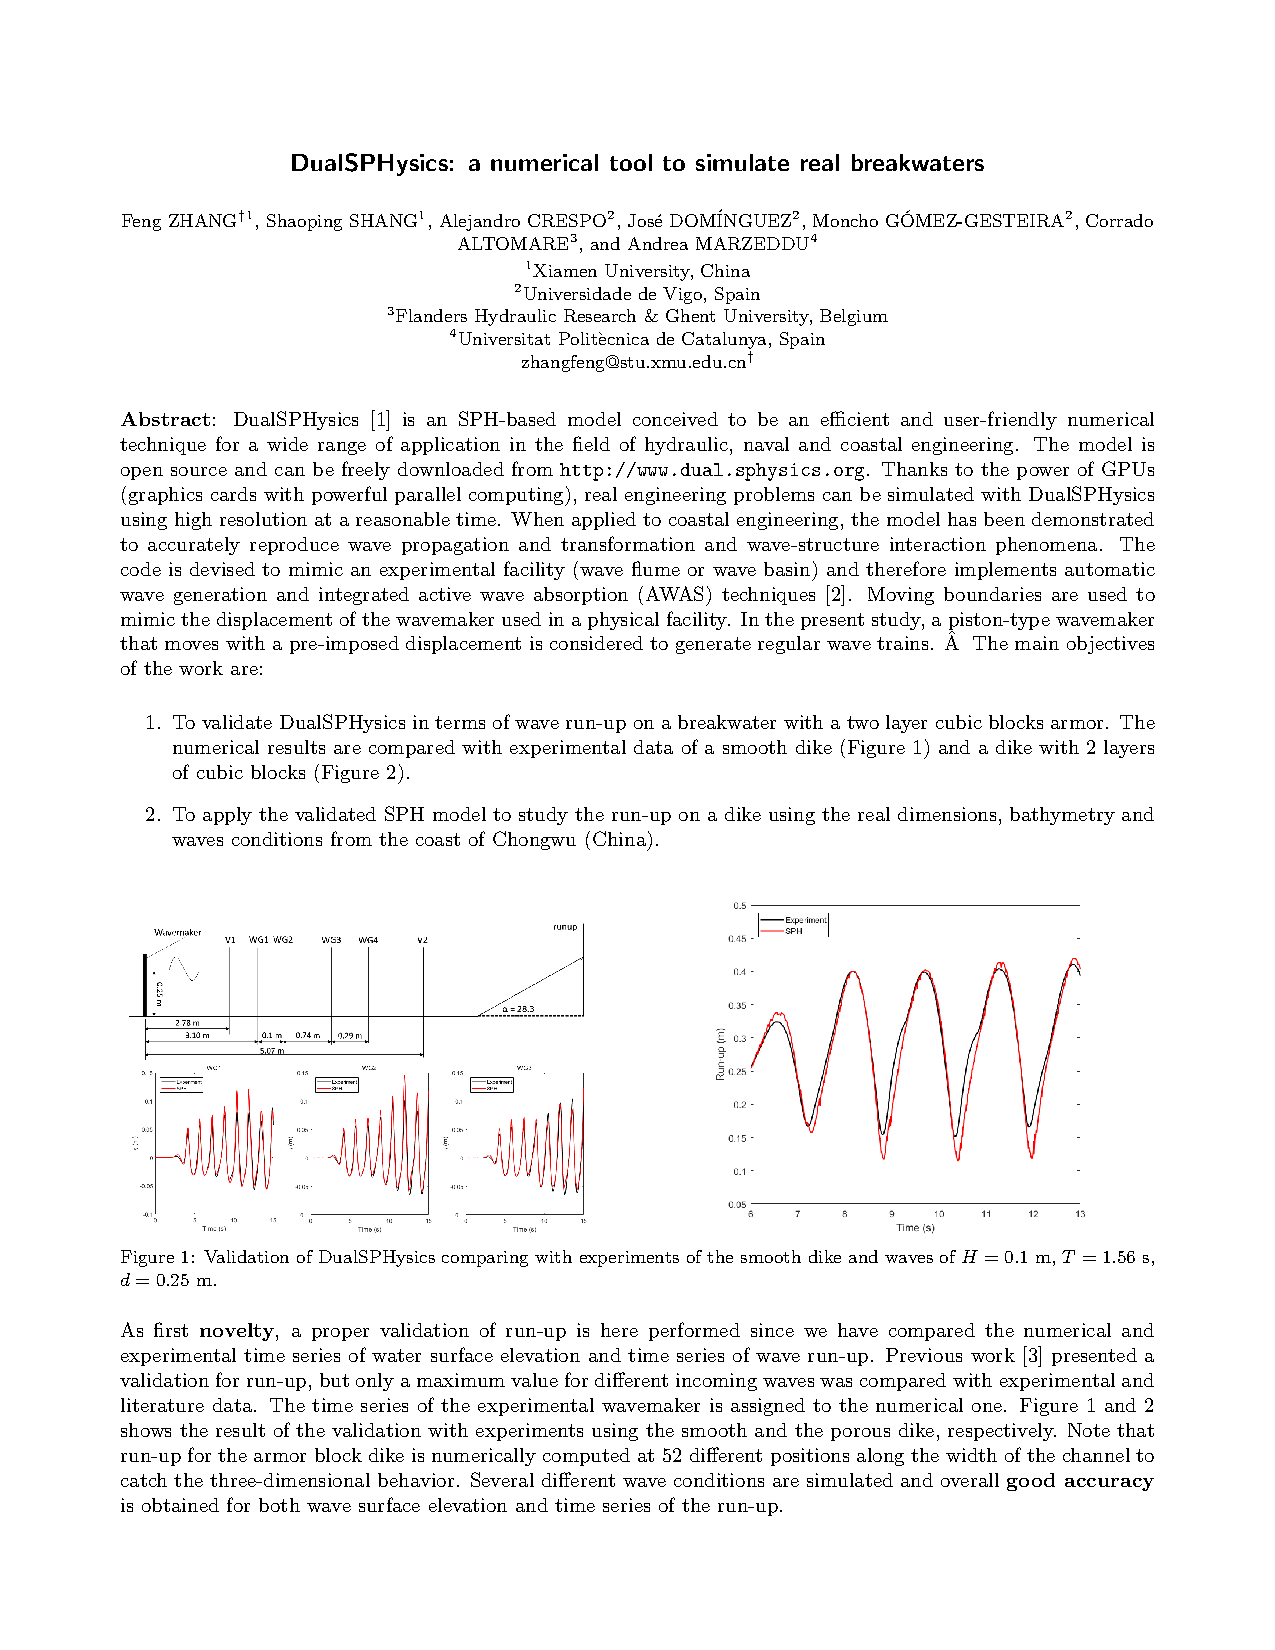
\includepdf[pages=-,pagecommand={\pagestyle{fancy}\label{1.1}},addtotoc={
     1,section,1,{~~~~~~~~Maritime and Naval Architecture Applications},p1,   
     1,subsection,1,DualSPHysics: a numerical tool to simulate real breakwaters,p1}]{abstract/pdfs/22.pdf}
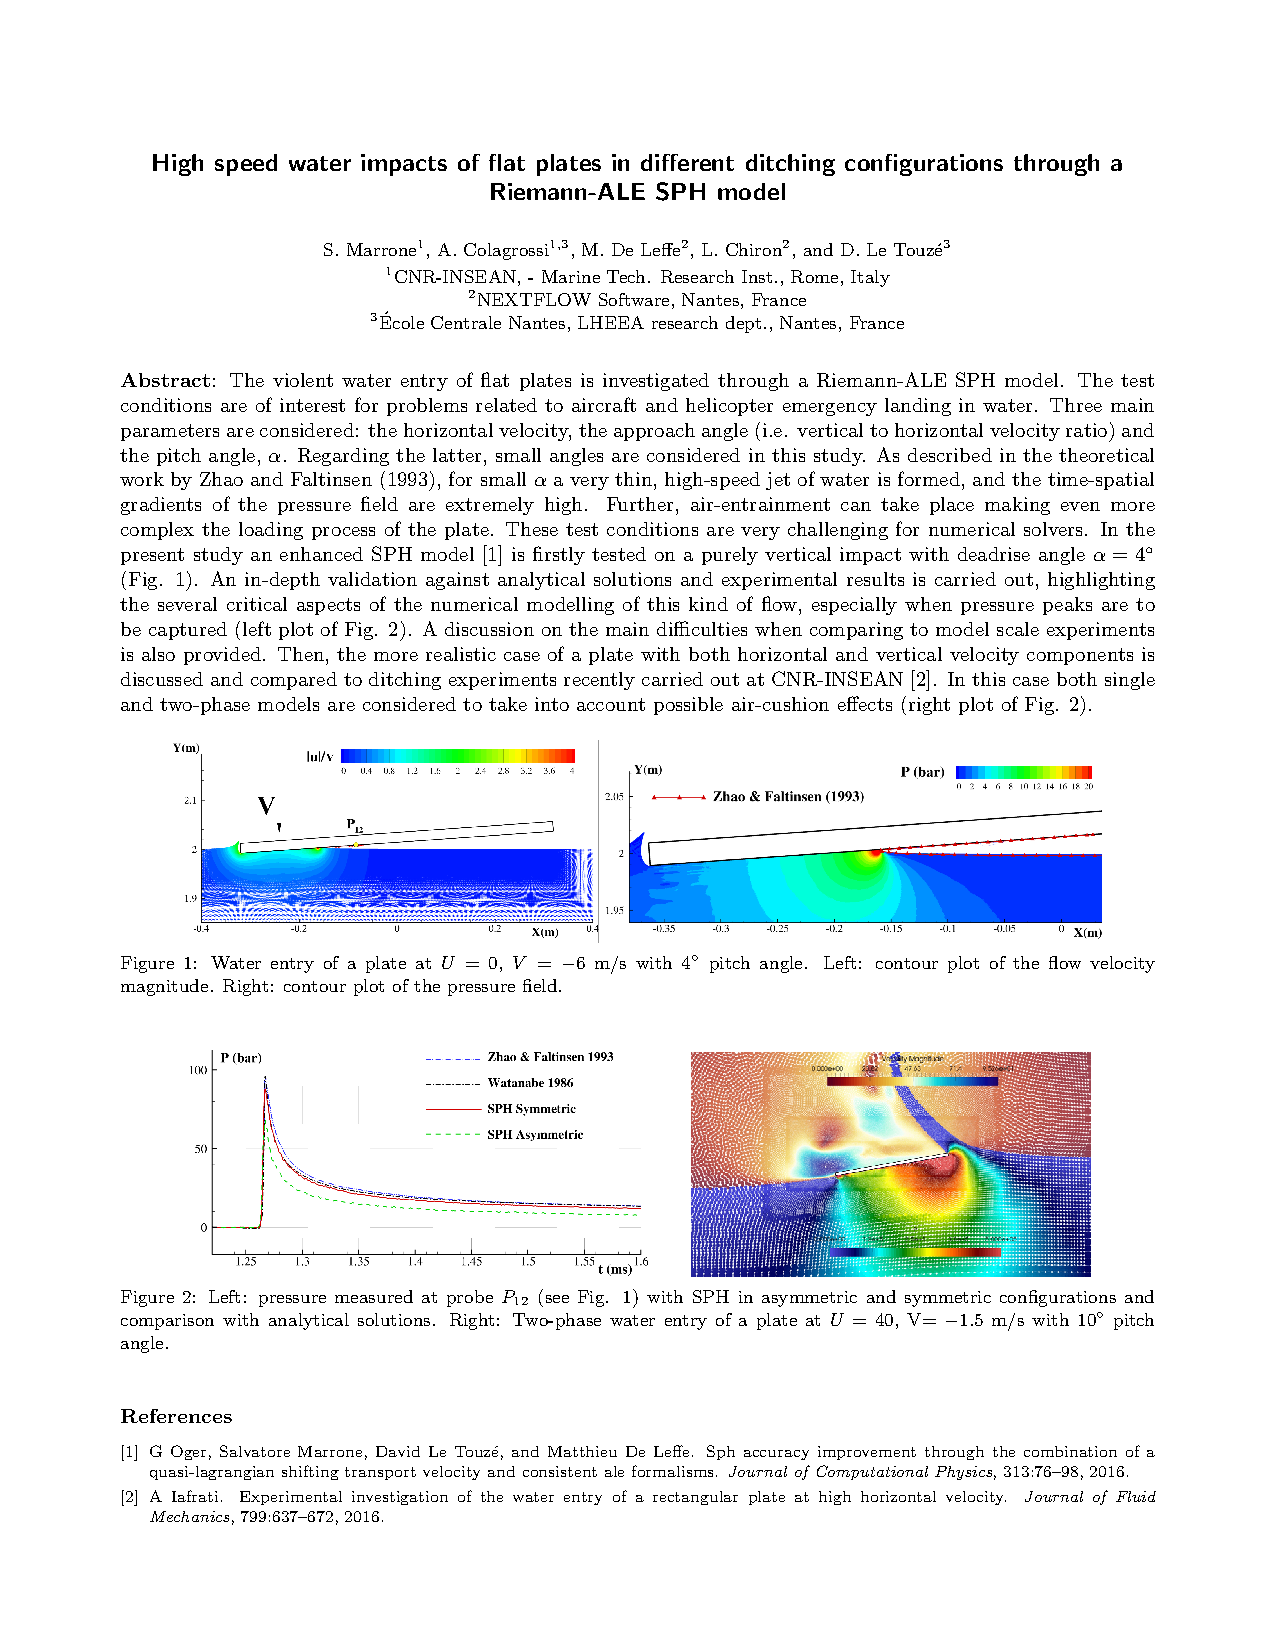
\includepdf[pages=-,pagecommand={\pagestyle{fancy}\label{1.2}},addtotoc={
     1,subsection,1,High speed water impacts of fat plates in different ditching configurations through a Riemann-ALE SPH model,p1}]{abstract/pdfs/1.pdf}
%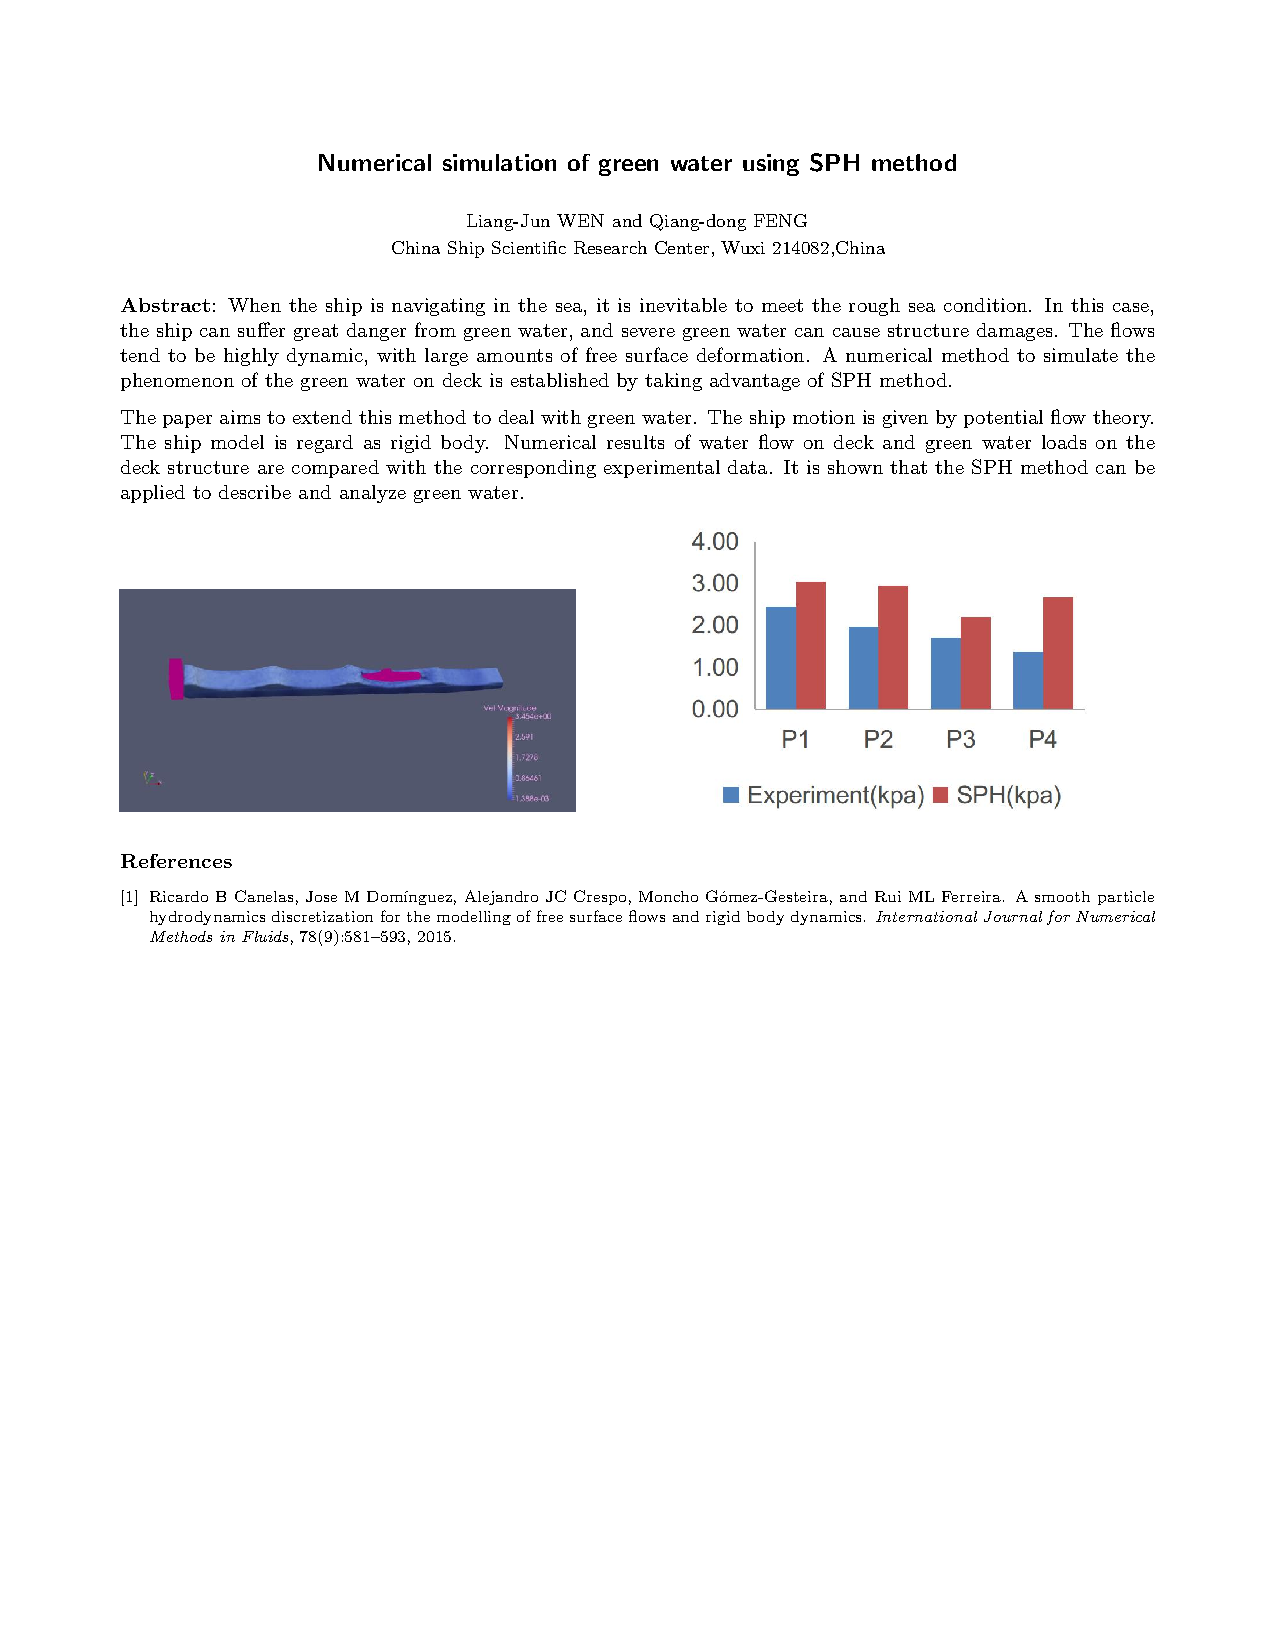
\includepdf[pages=-,pagecommand={\pagestyle{fancy}\label{1.2}},addtotoc={  
%     1,subsection,1,Numerical simulation of green water using SPH method,p1}]{abstract/pdfs/32.pdf}
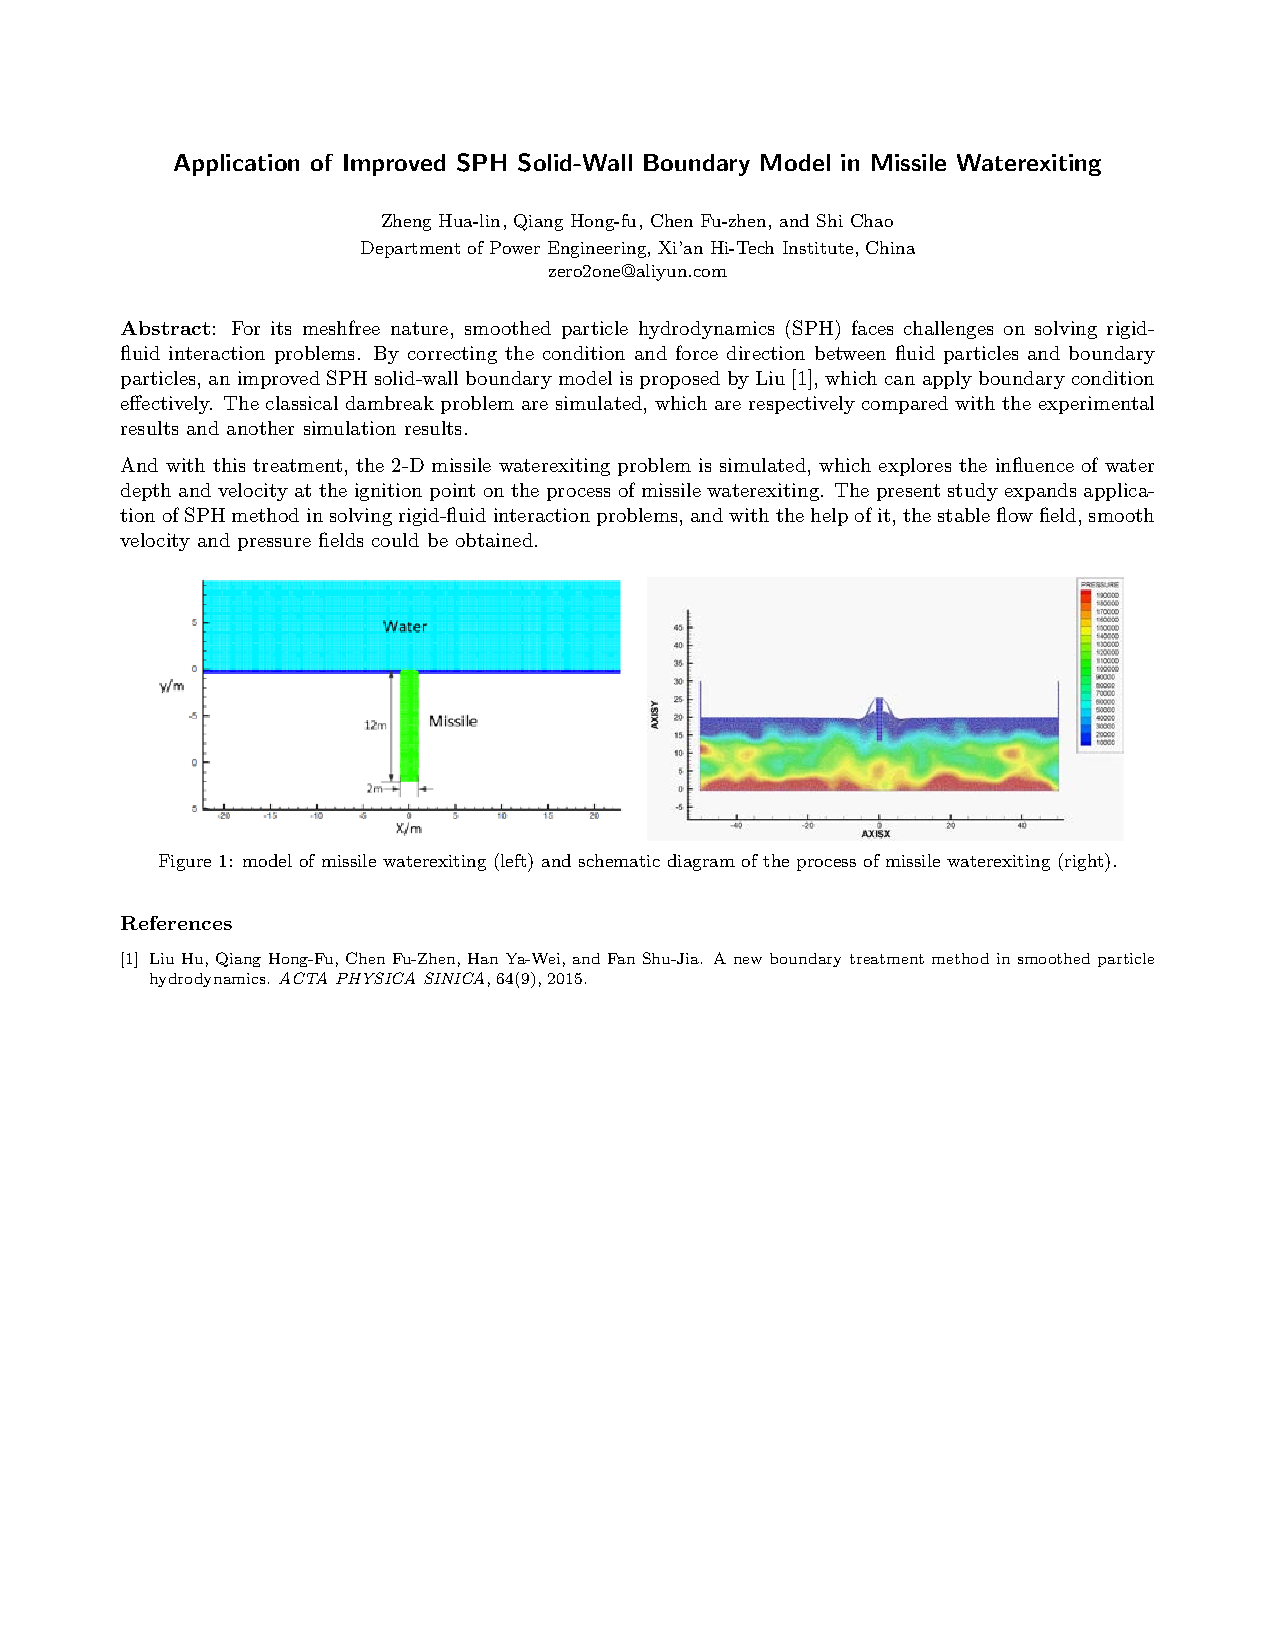
\includepdf[pages=-,pagecommand={\pagestyle{fancy}\label{1.3}},addtotoc={  
     1,subsection,1,Application of improved SPH solid-wall boundary model in missile waterexiting,p1}]{abstract/pdfs/36.pdf}


%\section{Session 2: Multiple Continua and Multi-Phase Flows}
%2.1: 24
%2.2: 31
%2.3: 39
%2.4: 21

\rhead{Session 2}
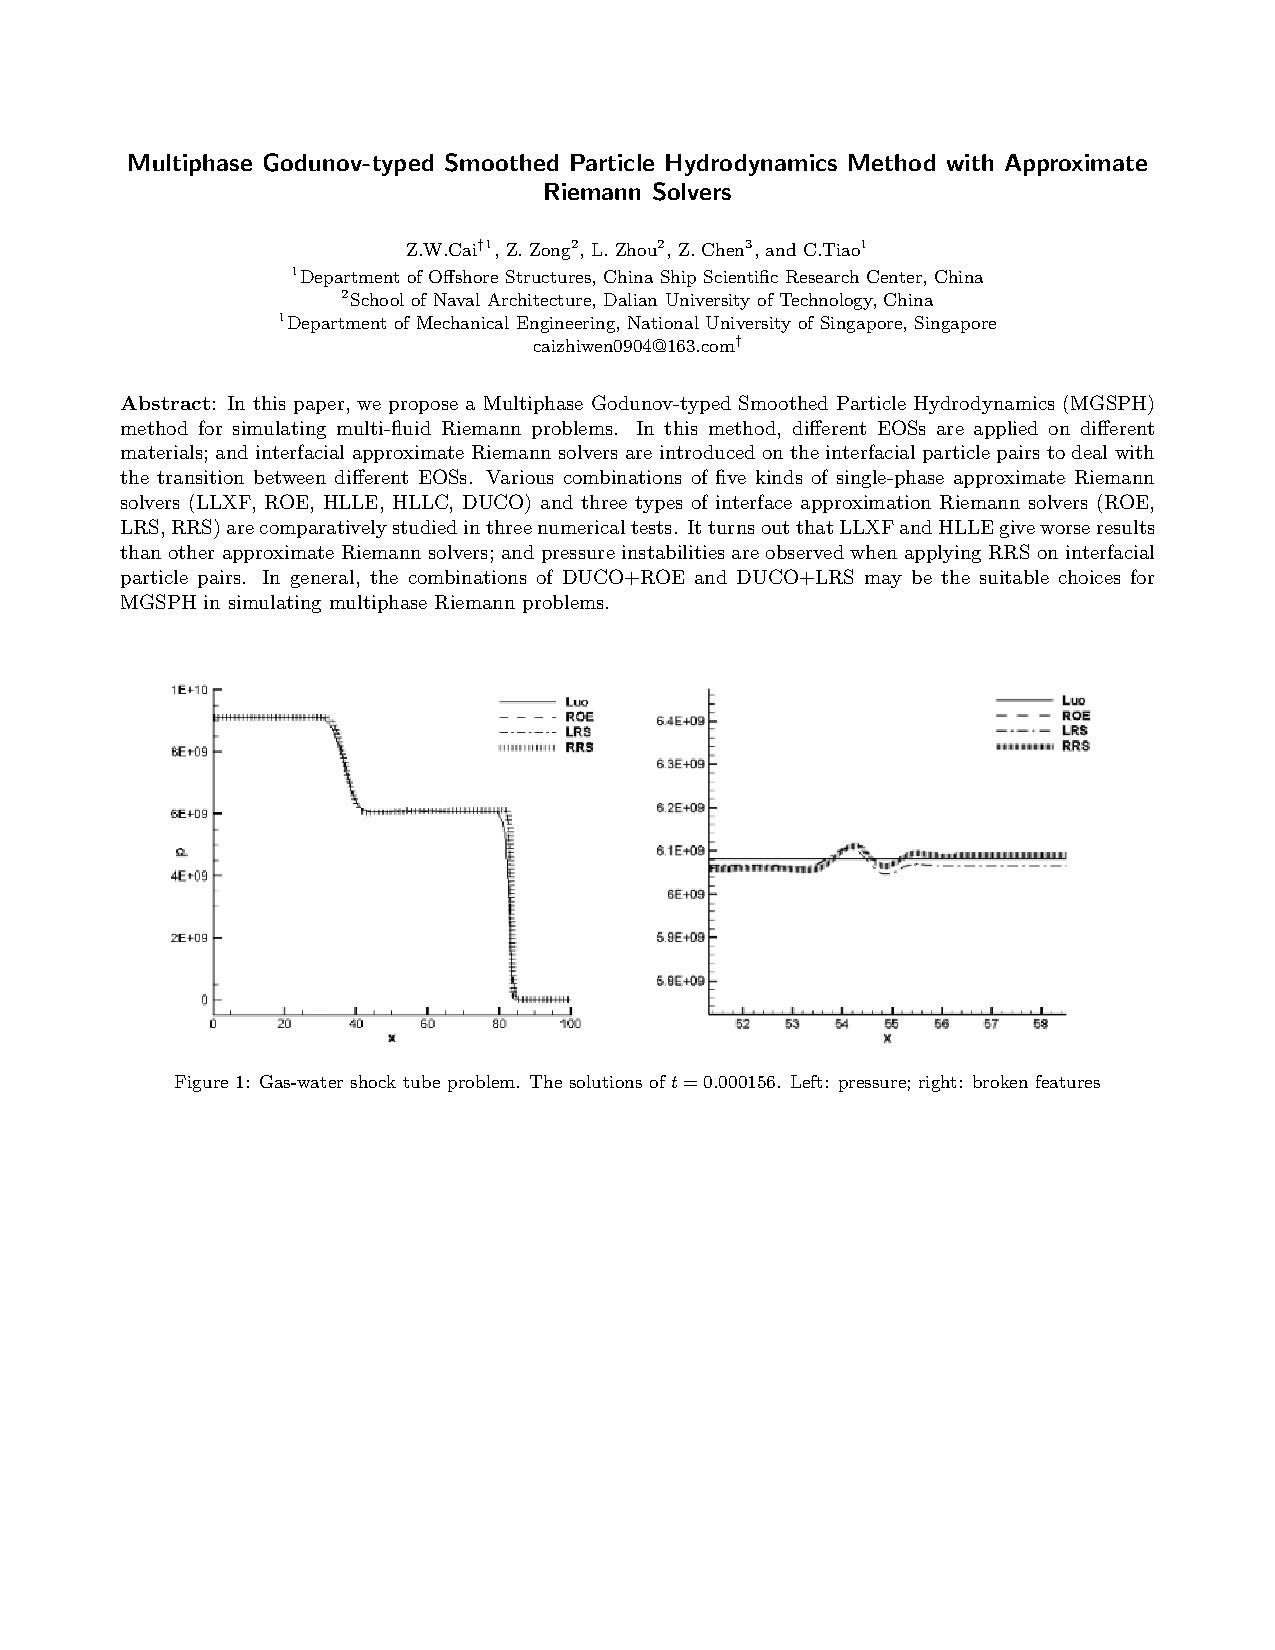
\includepdf[pages=-,pagecommand={\pagestyle{fancy}\label{2.1}},addtotoc={
     1,section,1,{~~~~~~~~Multiple Continua and Multi-Phase Flows},p1,   
     1,subsection,1,Multiphase Godunov-typed smoothed particle hydrodynamics method with approximate Riemann solvers,p1}]{abstract/pdfs/24.pdf}
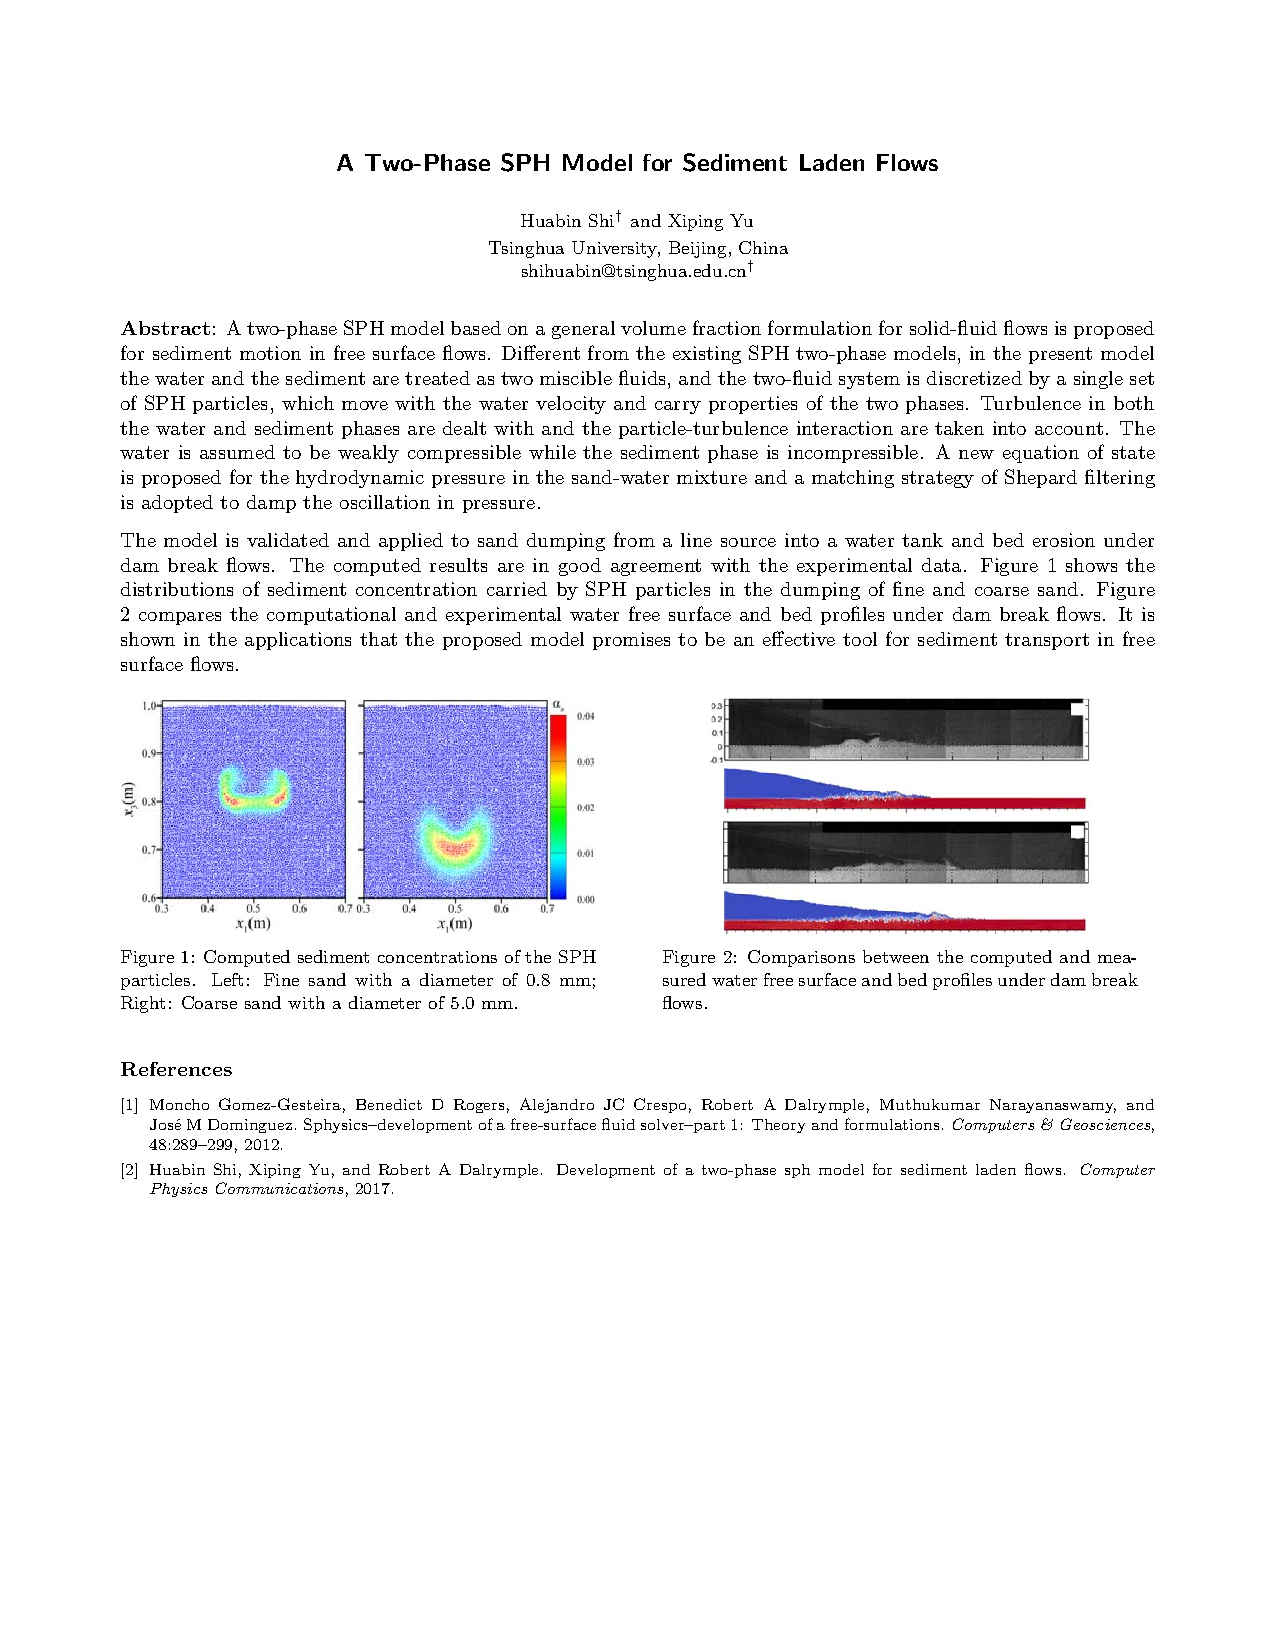
\includepdf[pages=-,pagecommand={\pagestyle{fancy}\label{2.2}},addtotoc={  
     1,subsection,1,A two-phase SPH model for sediment laden flows,p1}]{abstract/pdfs/31.pdf}
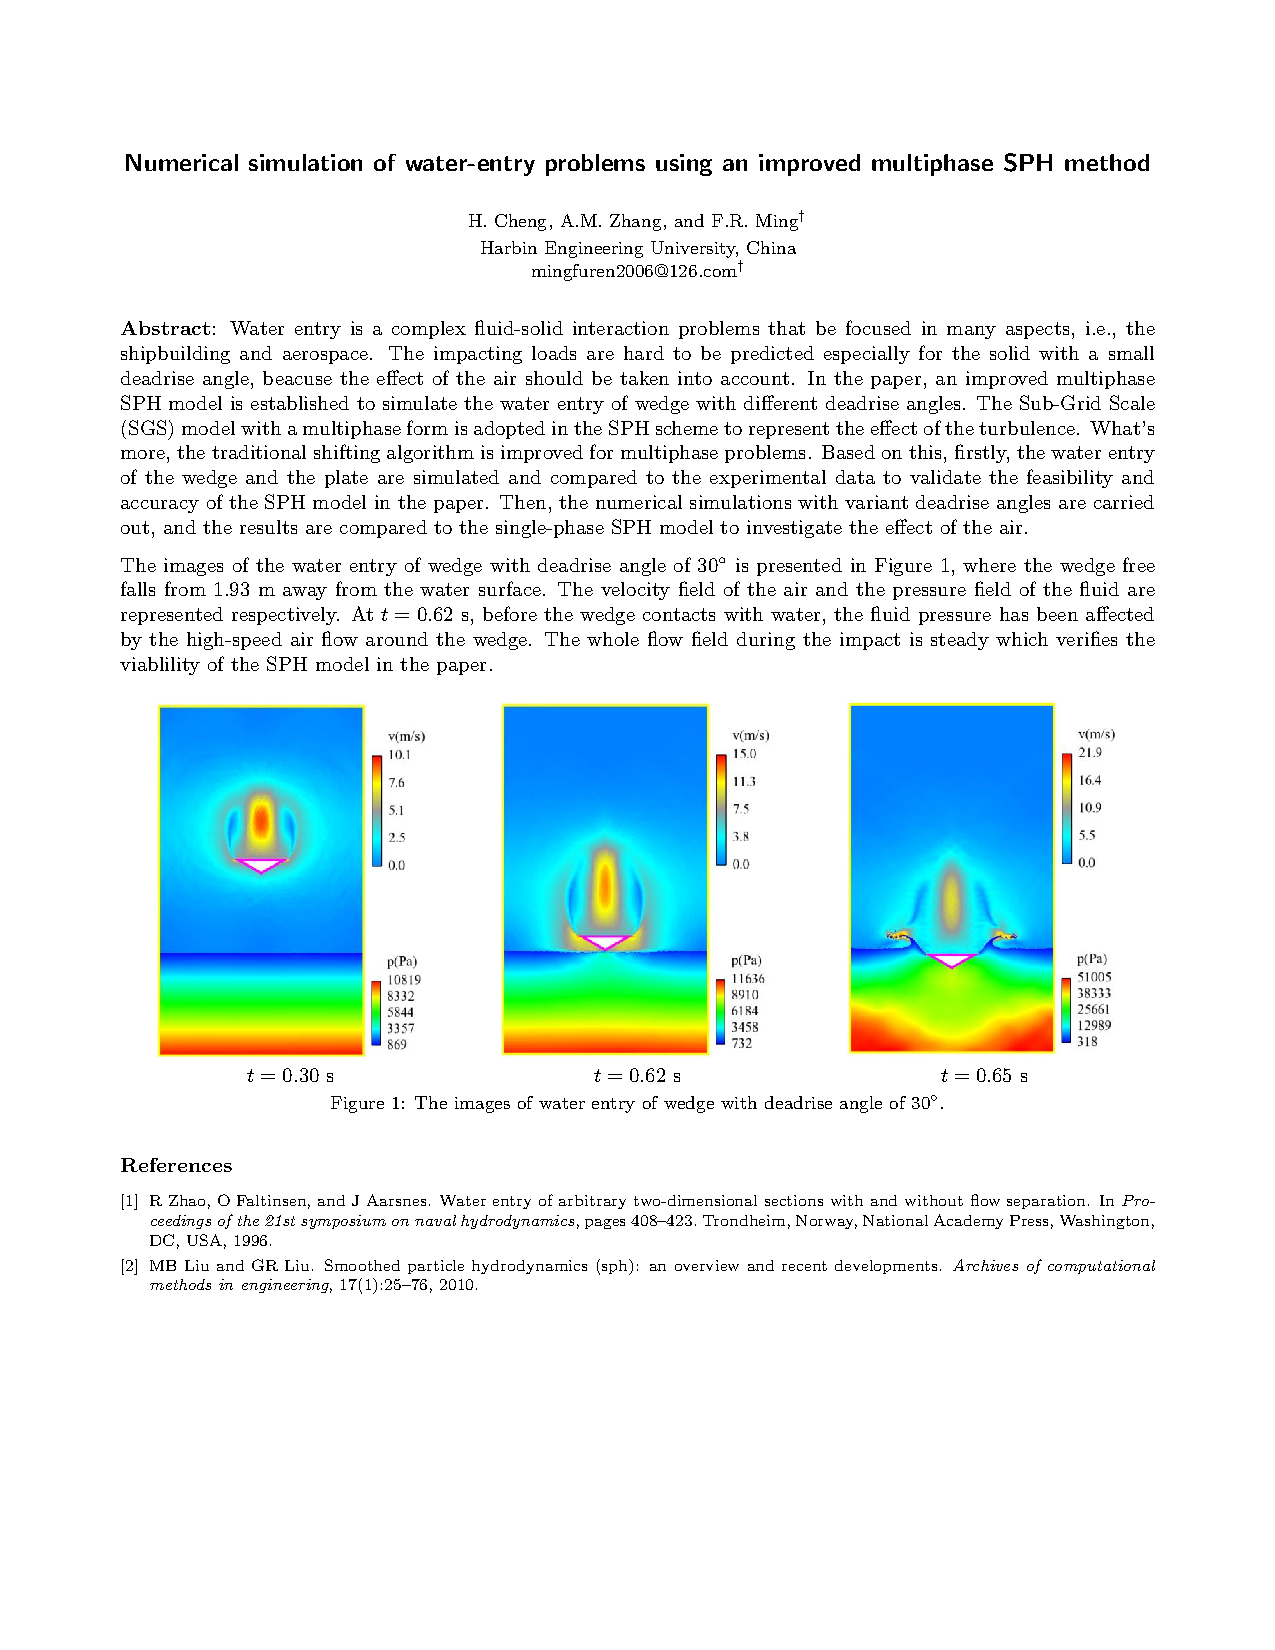
\includepdf[pages=-,pagecommand={\pagestyle{fancy}\label{2.3}},addtotoc={  
     1,subsection,1,Numerical simulation of water-entry problems using an improved multiphase SPH method,p1}]{abstract/pdfs/39.pdf}
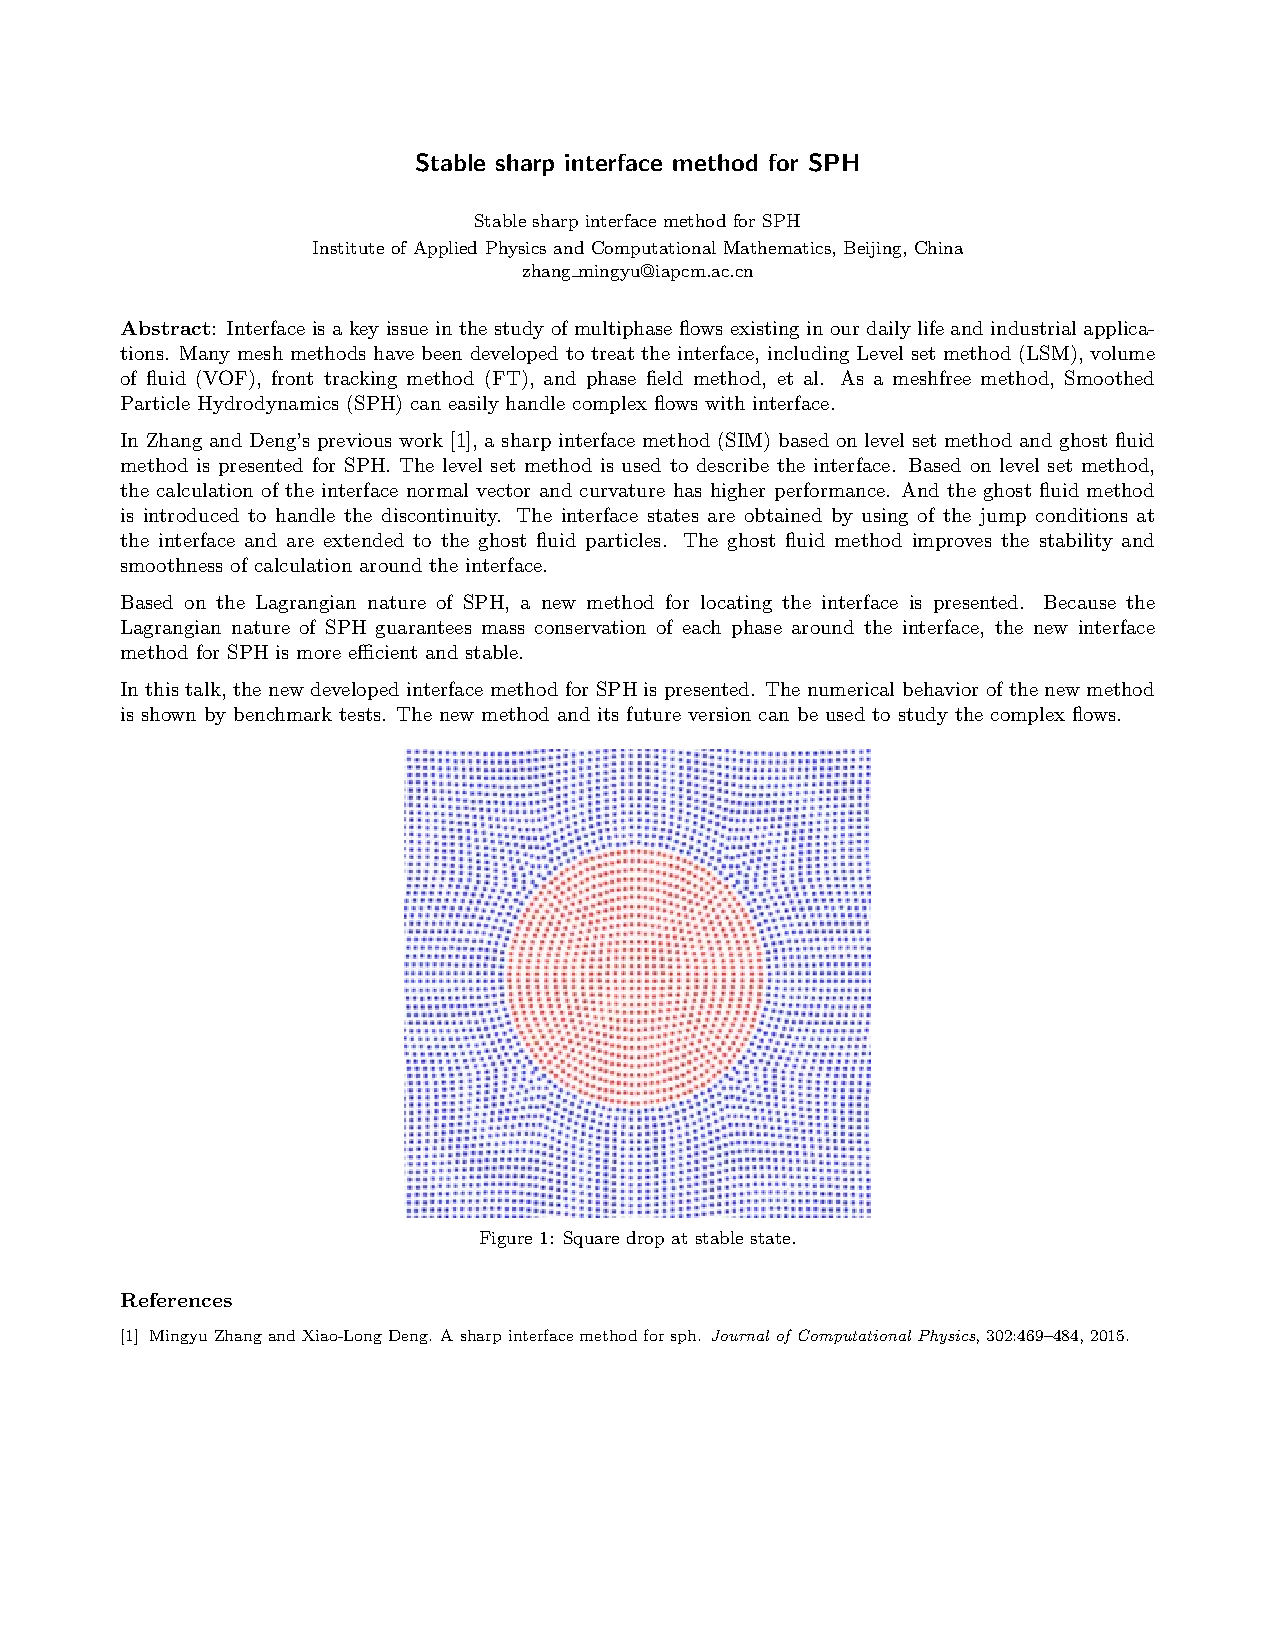
\includepdf[pages=-,pagecommand={\pagestyle{fancy}\label{2.4}},addtotoc={  
     1,subsection,1,Stable sharp interface method for SPH,p1}]{abstract/pdfs/21.pdf}

%\section{Session 3: Impacts with Fluids or Solids}
%3.1: 30
%3.2: 37
%3.3: 41
%3.4: 57

\rhead{Session 3}
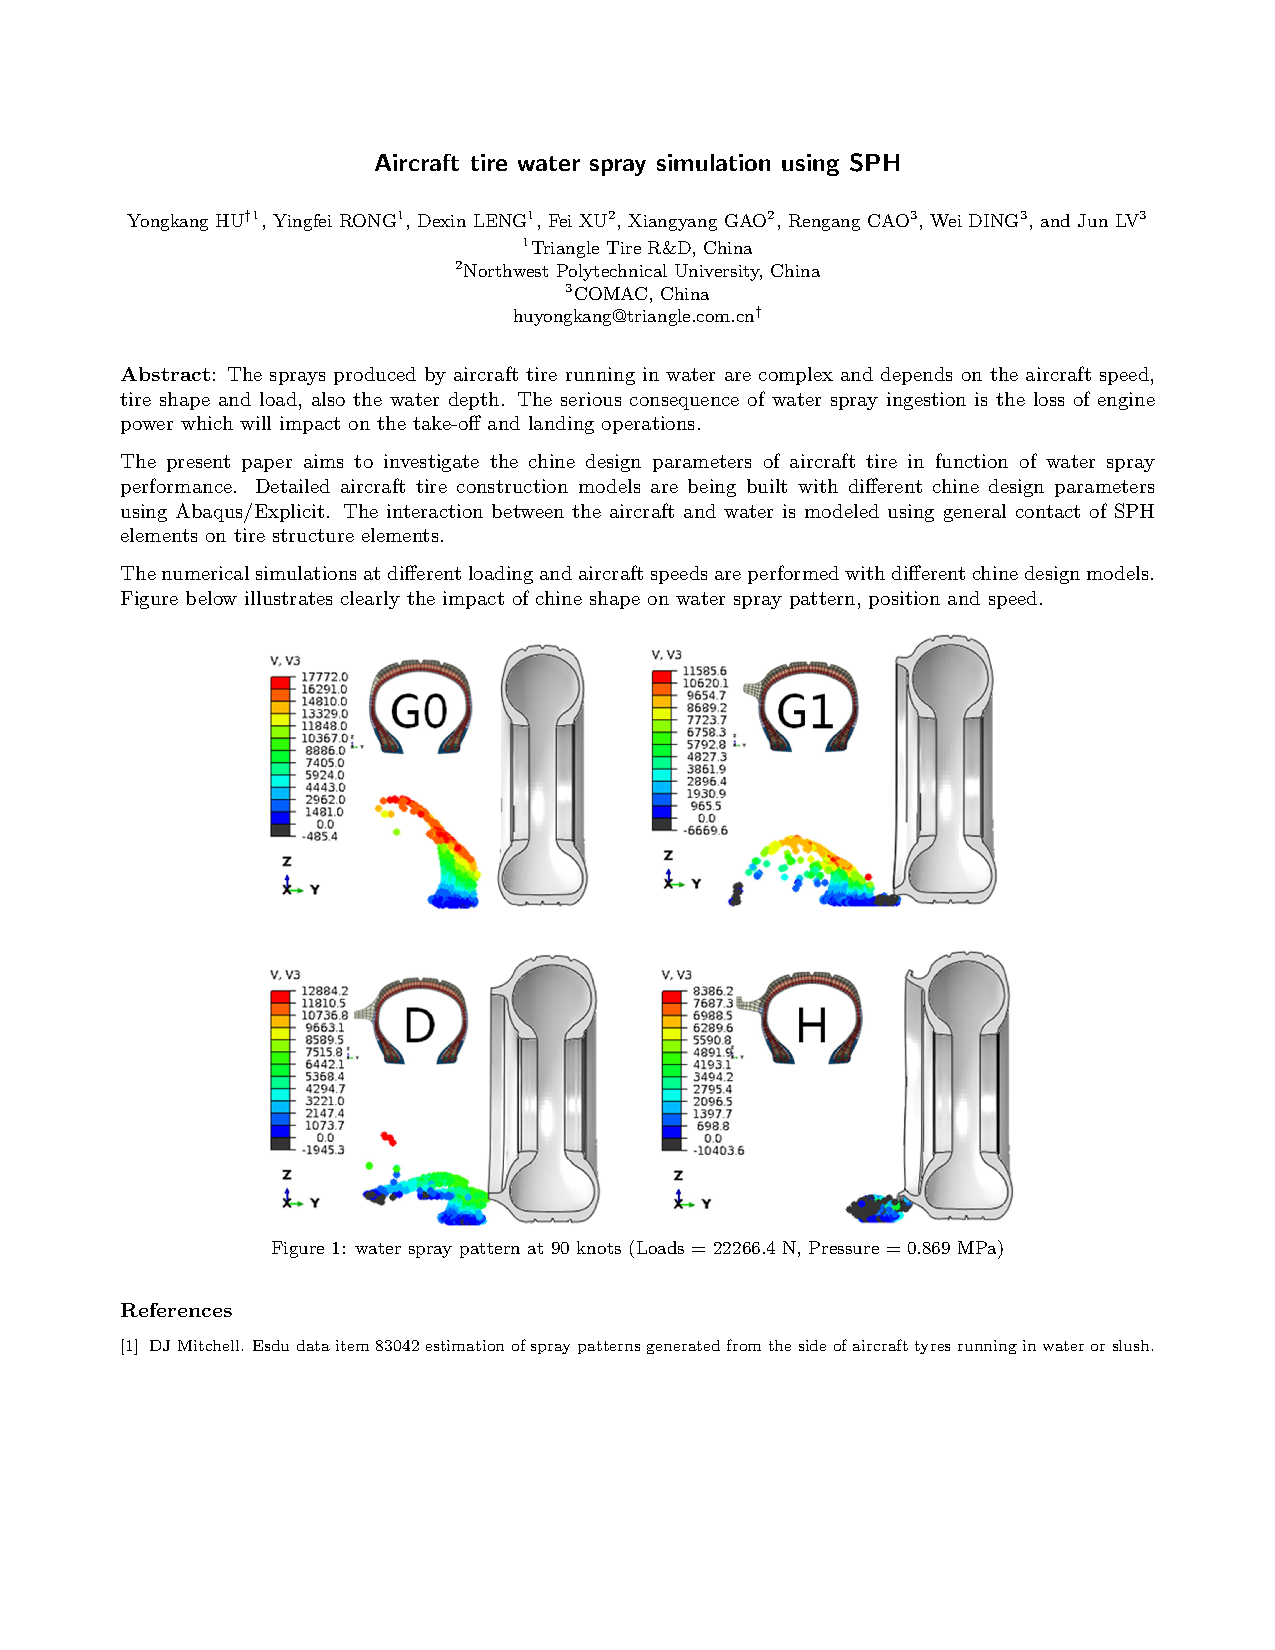
\includepdf[pages=-,pagecommand={\pagestyle{fancy}\label{3.1}},addtotoc={
     1,section,1,{~~~~~~~~Impacts with Fluids or Solids},p1,   
     1,subsection,1,Aircraft tire water spray simulation using SPH,p1}]{abstract/pdfs/30.pdf}
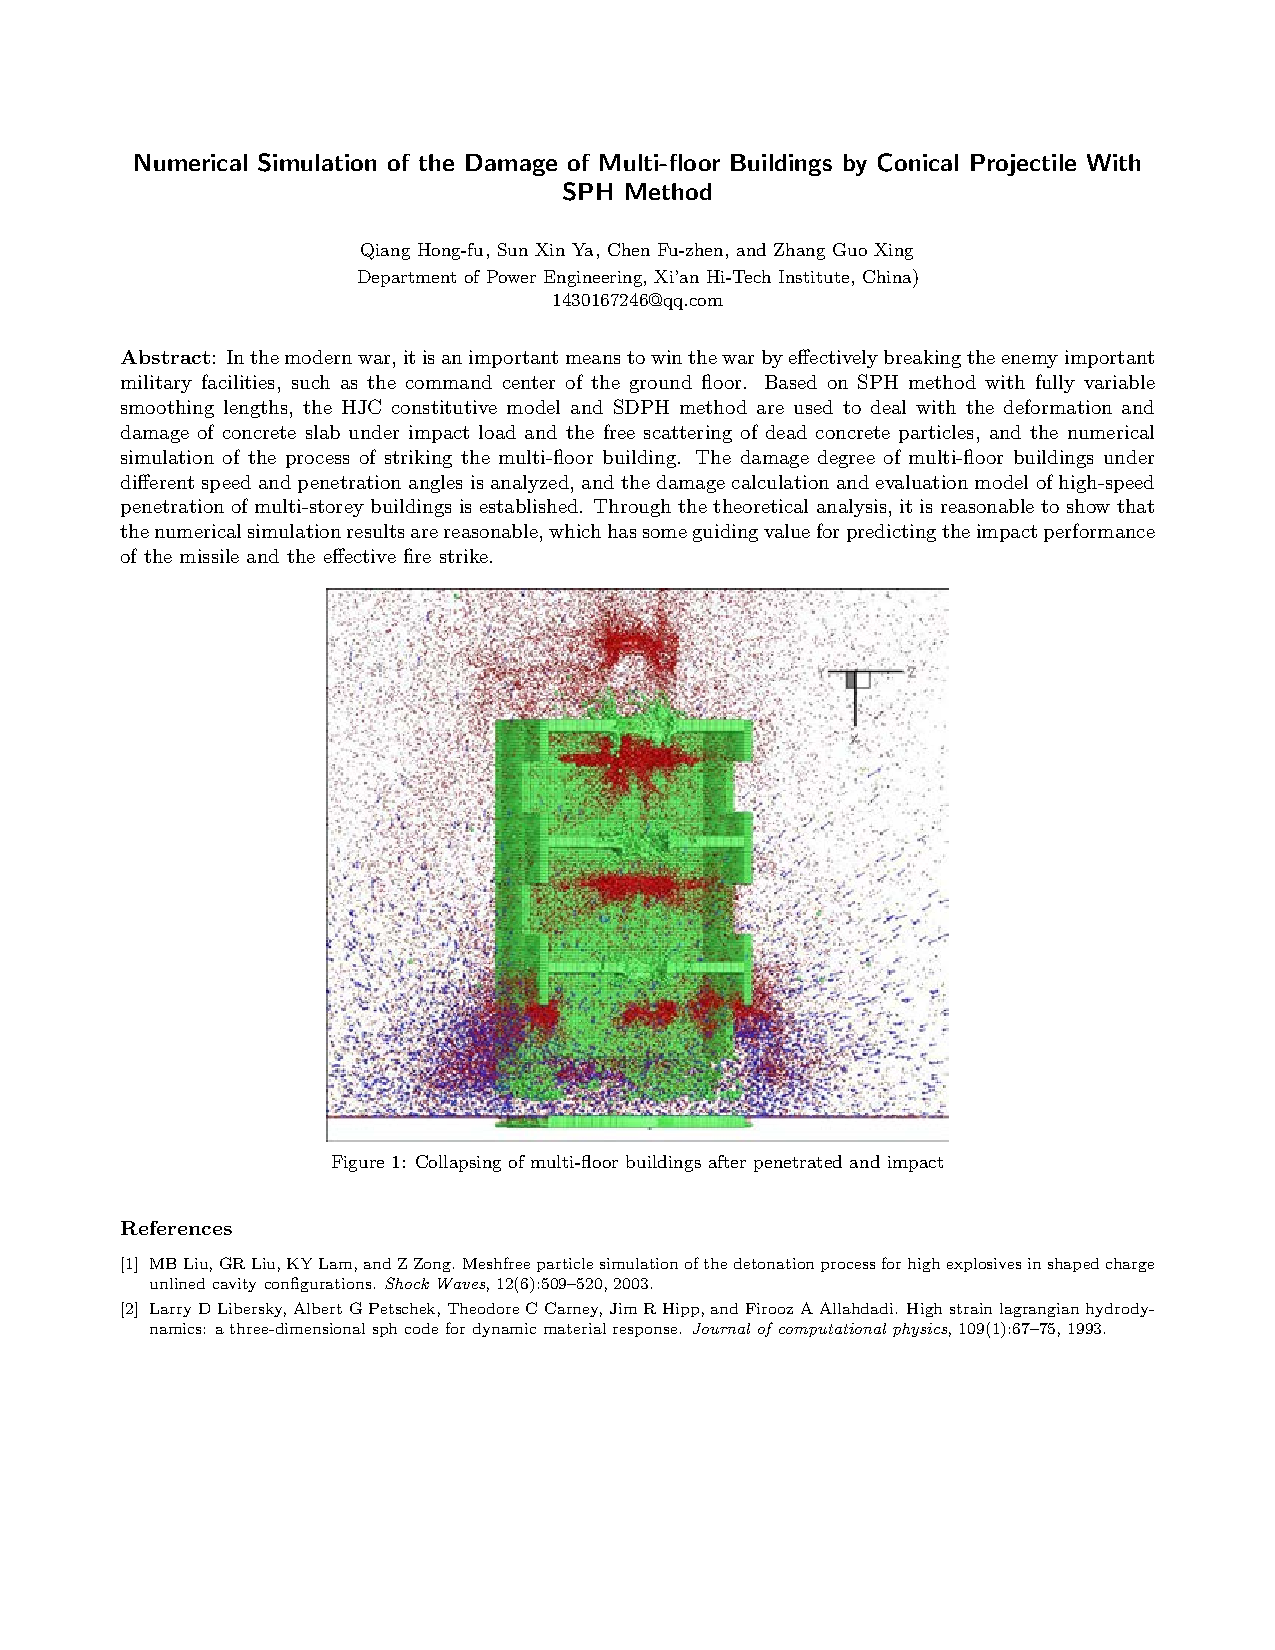
\includepdf[pages=-,pagecommand={\pagestyle{fancy}\label{3.2}},addtotoc={  
     1,subsection,1,Numerical simulation of the damage of multi-floor buildings by conical projectile with SPH method,p1}]{abstract/pdfs/37.pdf}
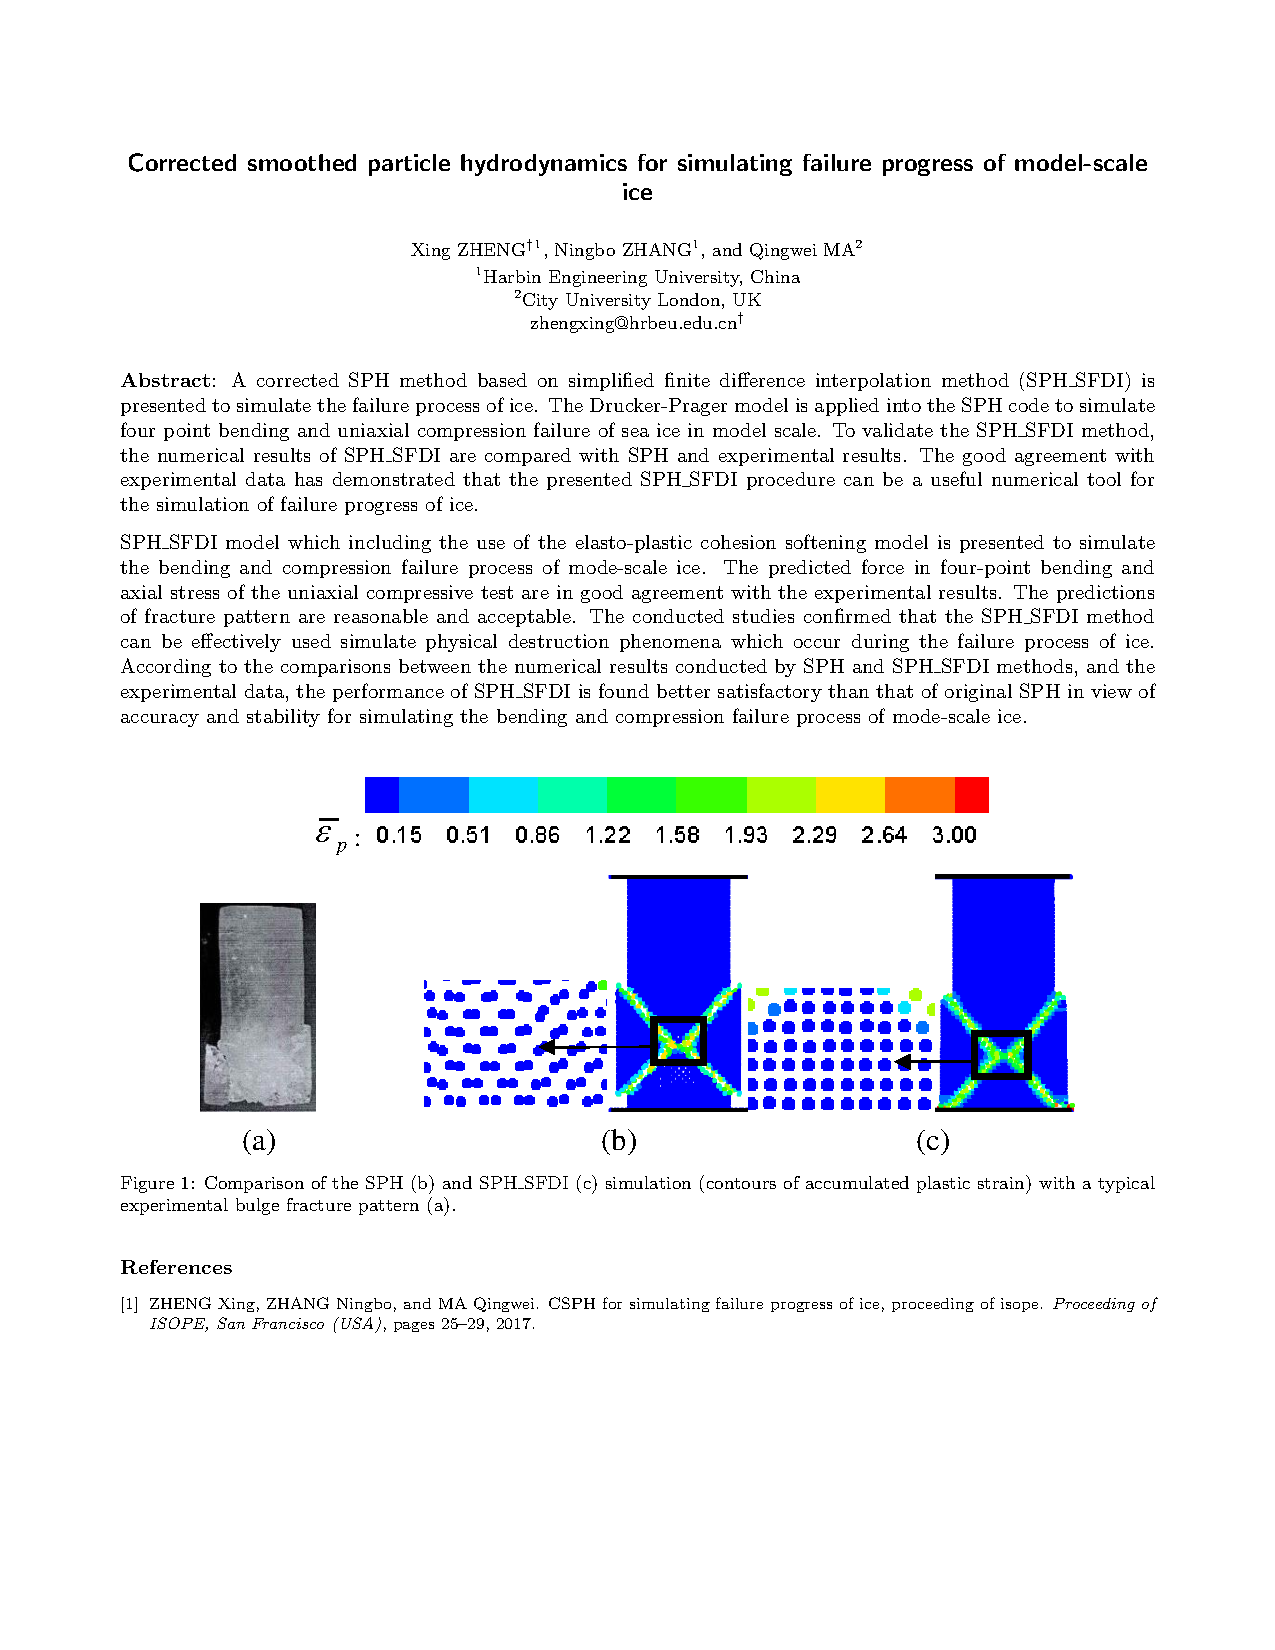
\includepdf[pages=-,pagecommand={\pagestyle{fancy}\label{3.3}},addtotoc={  
     1,subsection,1,Corrected smoothed particle hydrodynamics for simulating failure progress of model-scale ice,p1}]{abstract/pdfs/41.pdf}
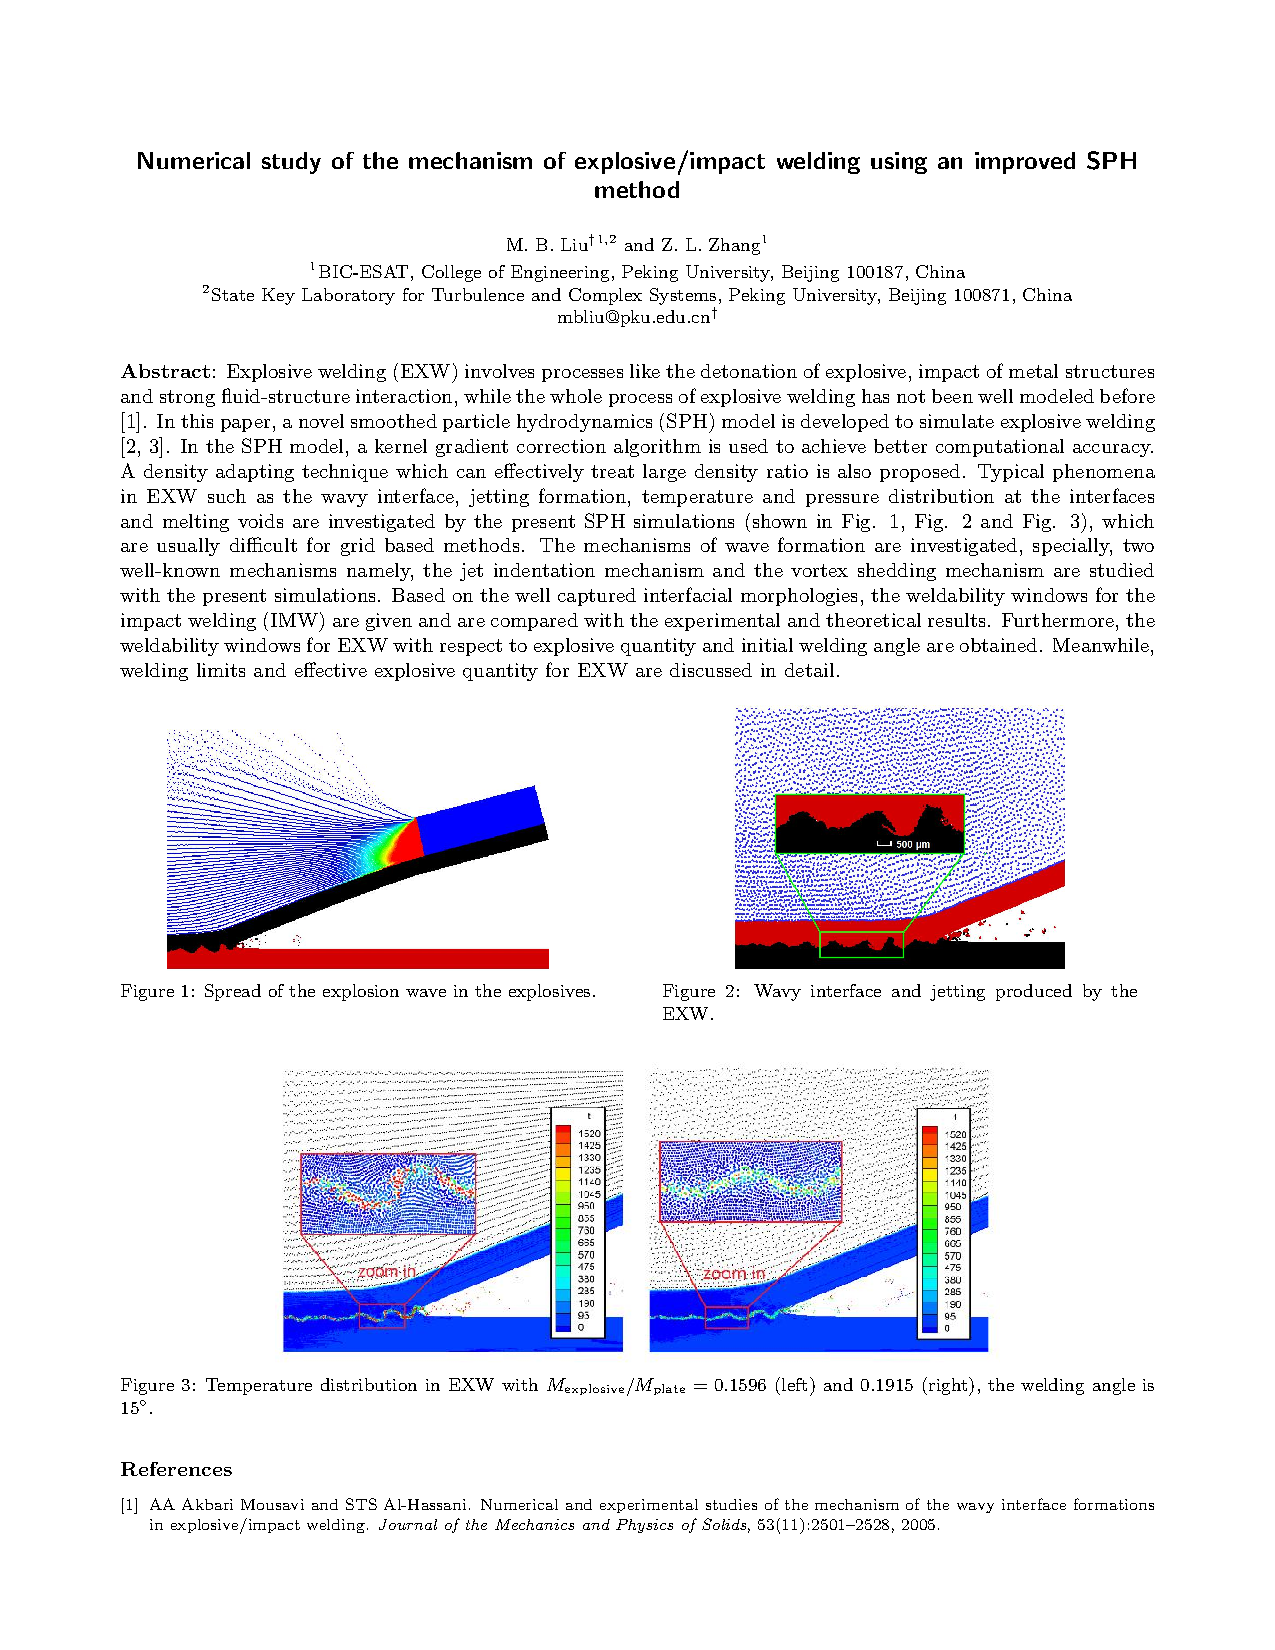
\includepdf[pages=-,pagecommand={\pagestyle{fancy}\label{3.4}},addtotoc={  
     1,subsection,1,Numerical study of the mechanism of explosive/impact welding using an improved SPH method,p1}]{abstract/pdfs/57.pdf}

%\section{Session 4: Free Surface and Moving Boundaries Applications}
%4.1: 1
%4.2: 14
%4.3: 40
%4.4: 44

\rhead{Session 4}
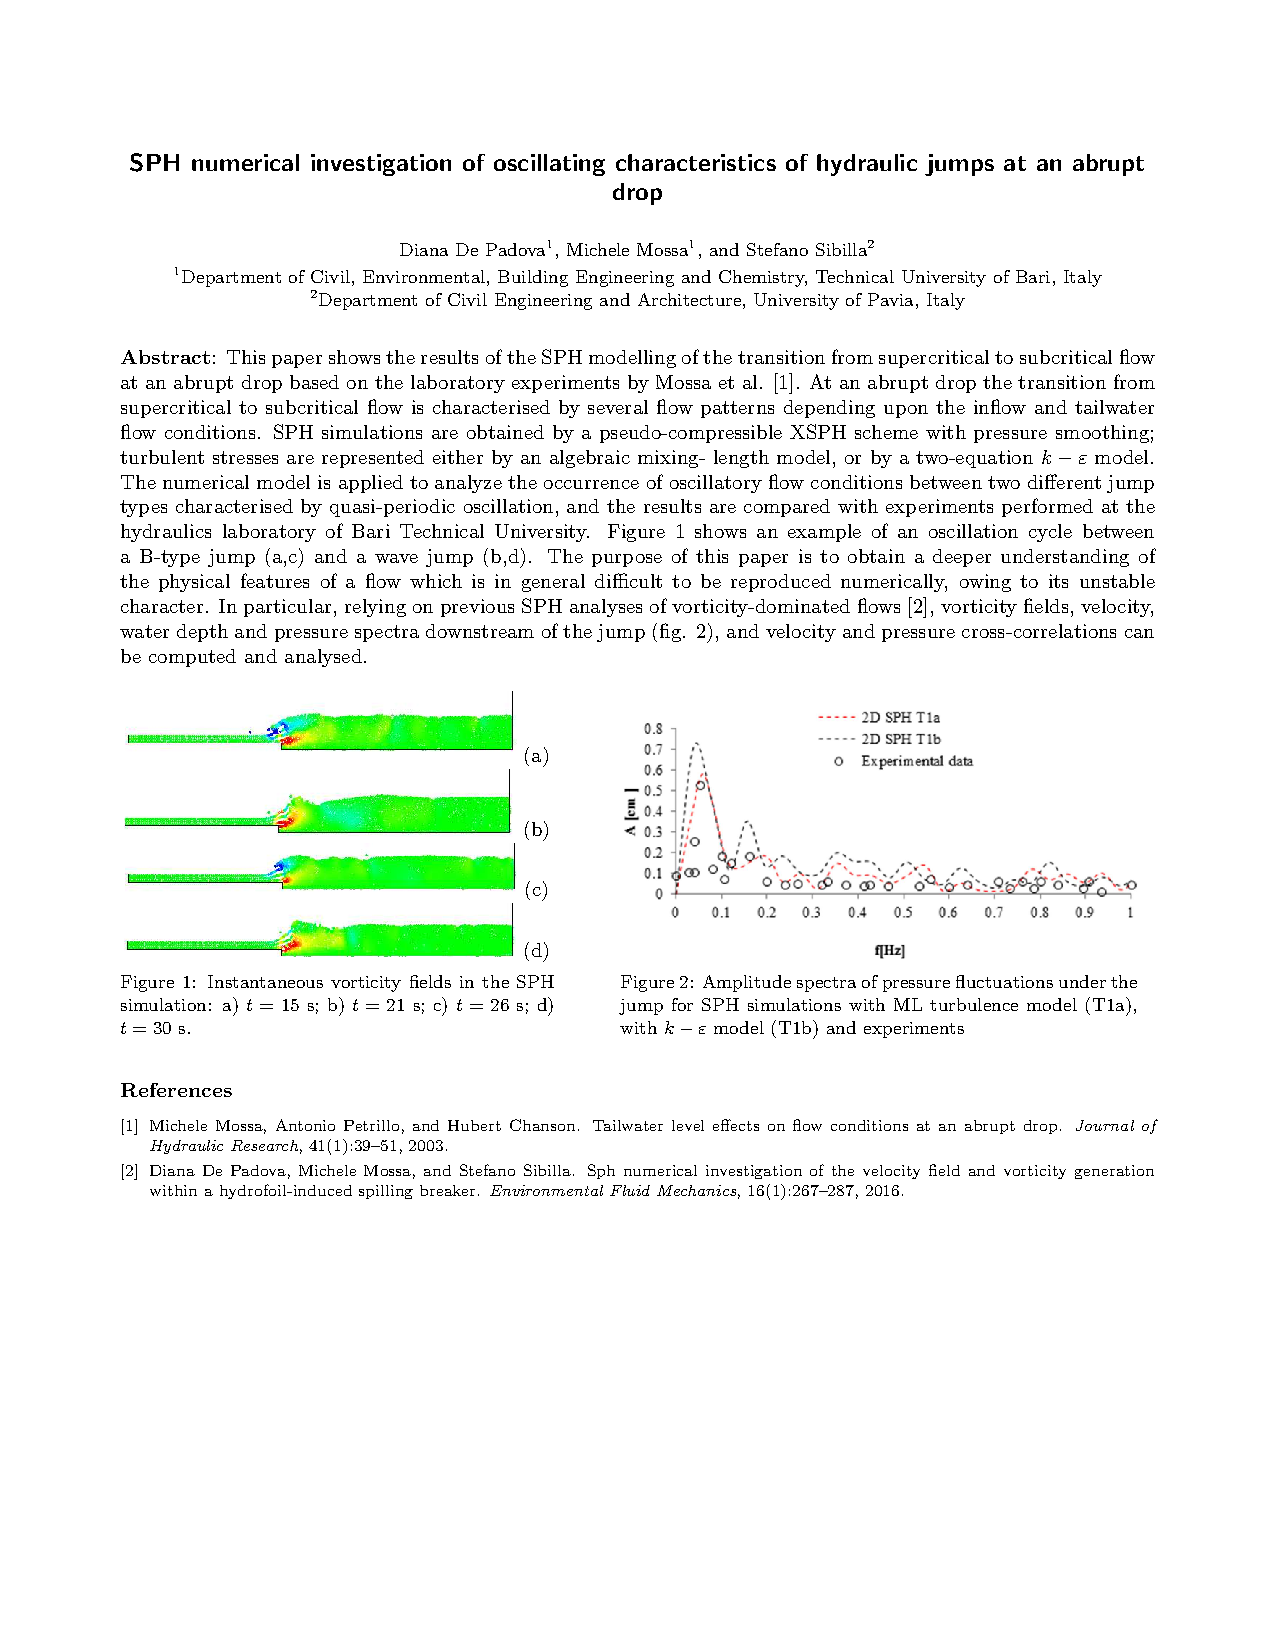
\includepdf[pages=-,pagecommand={\pagestyle{fancy}\label{4.1}},addtotoc={  
     1,section,1,{~~~~~~~~Free Surface and Moving Boundaries Applications},p1,   
     1,subsection,1,SPH numerical investigation of oscillating characteristics of hydraulic jumps at an abrupt drop,p1}]{abstract/pdfs/14.pdf}

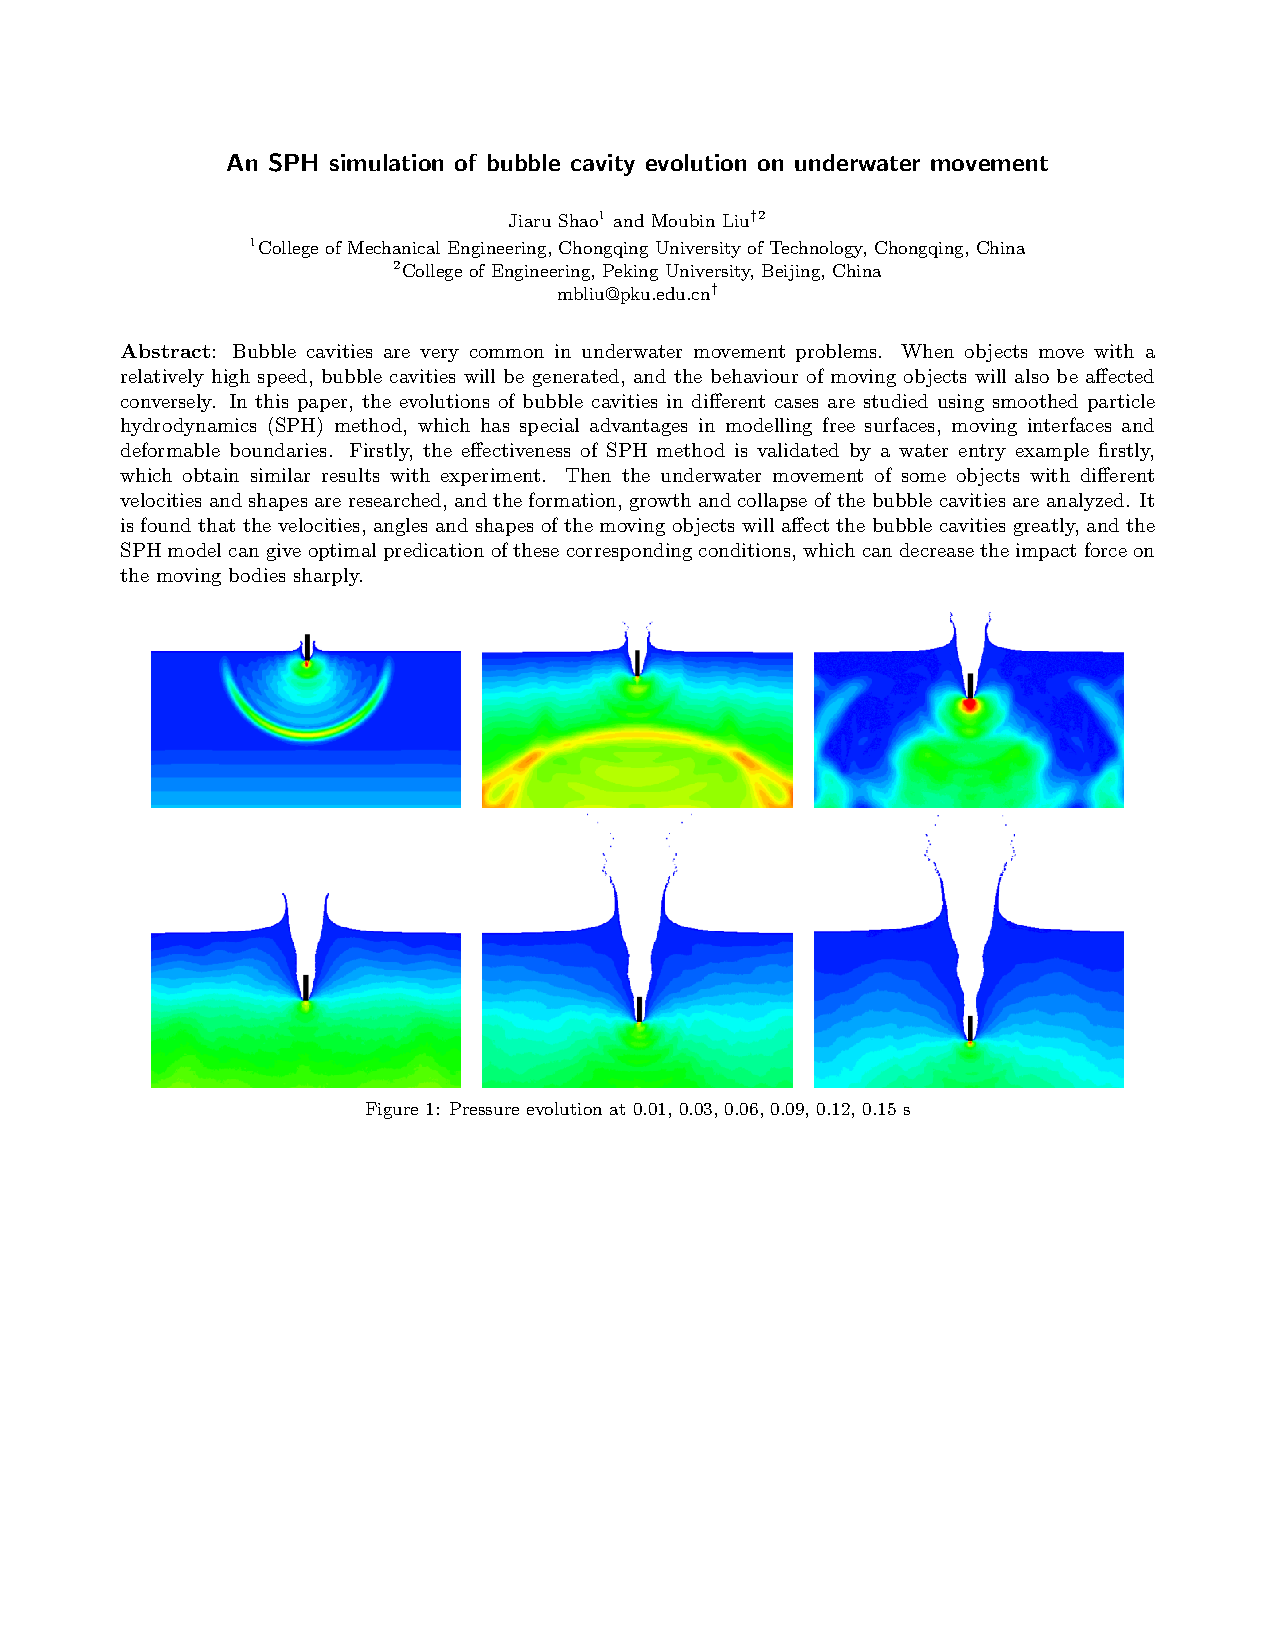
\includepdf[pages=-,pagecommand={\pagestyle{fancy}\label{4.2}},addtotoc={  
     1,subsection,1,An SPH simulation of bubble cavity evolution on underwater movement,p1}]{abstract/pdfs/20.pdf}
     
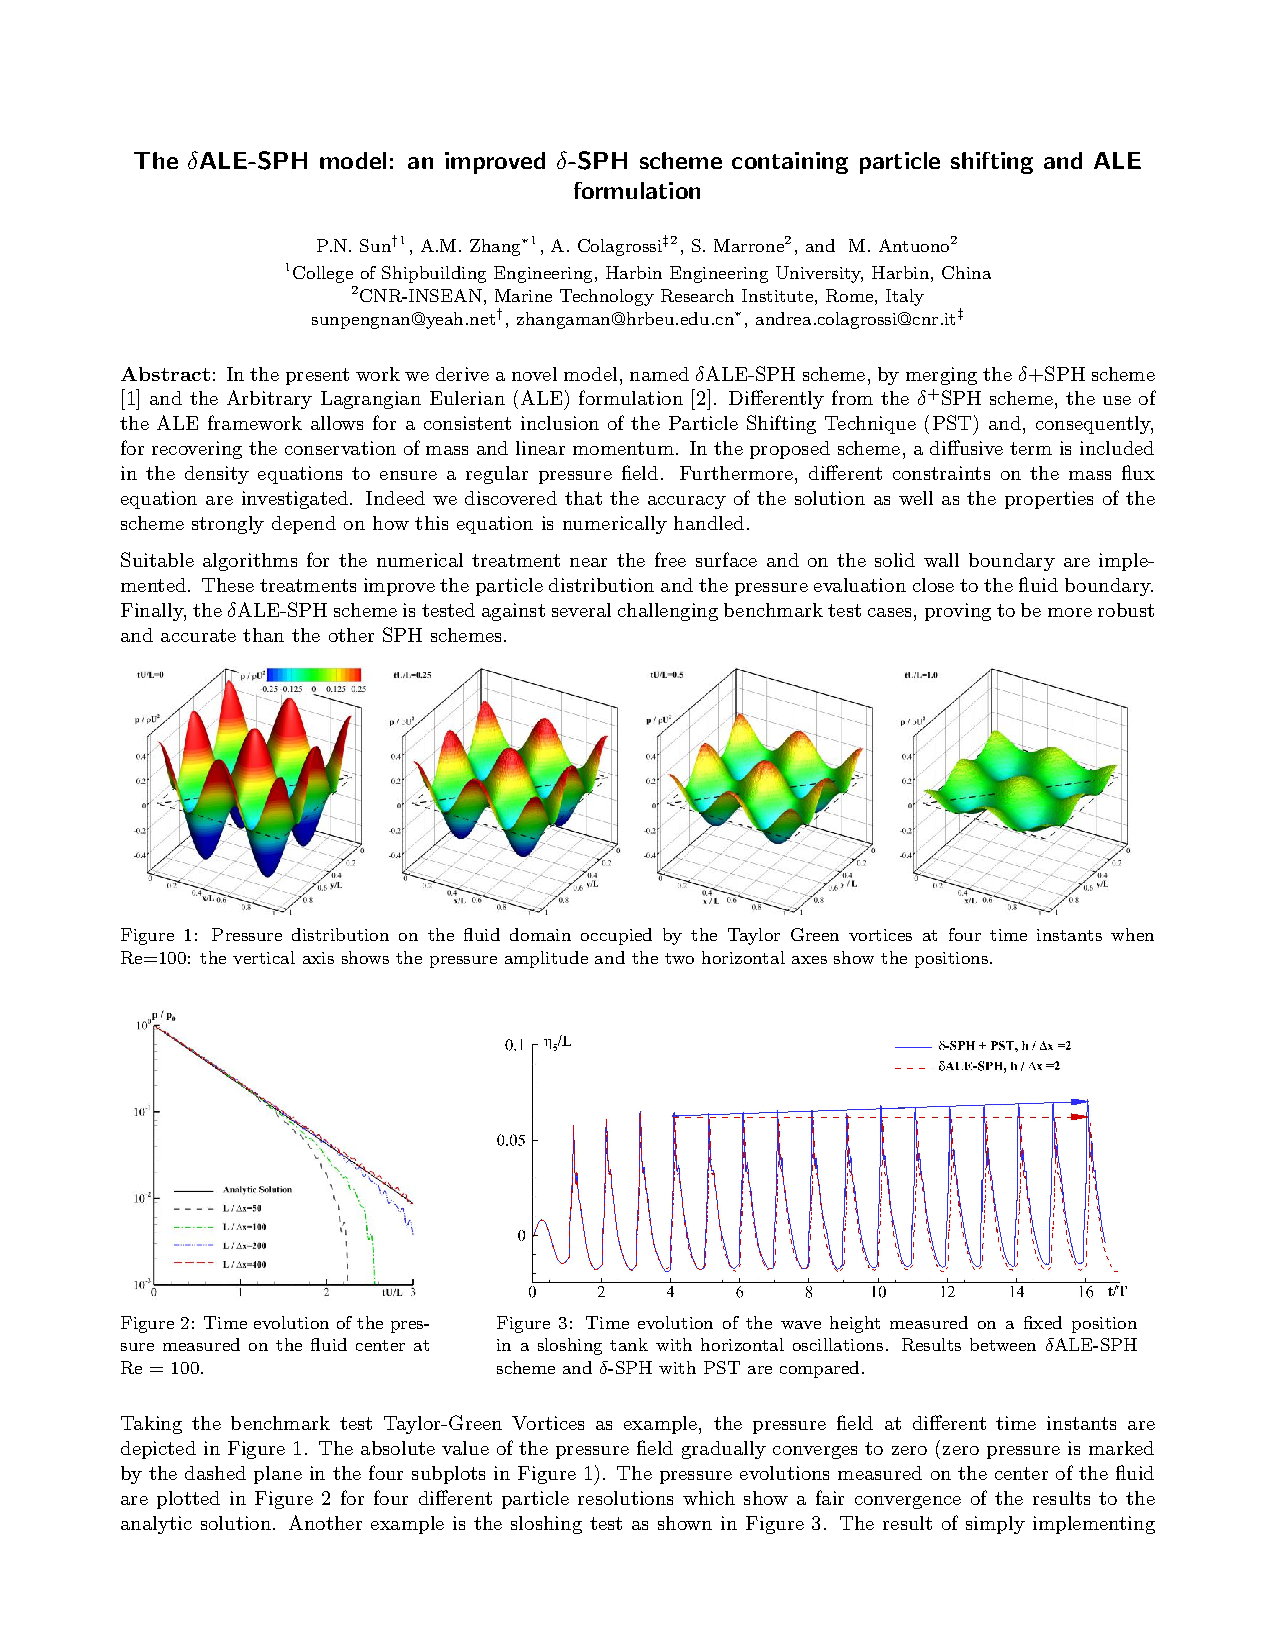
\includepdf[pages=-,pagecommand={\pagestyle{fancy}\label{4.3}},addtotoc={  
     1,subsection,1,The $\delta$ALE-SPH model: an improved $\delta$-SPH scheme containing particle shifting and ALE formulation,p1}]{abstract/pdfs/40.pdf}
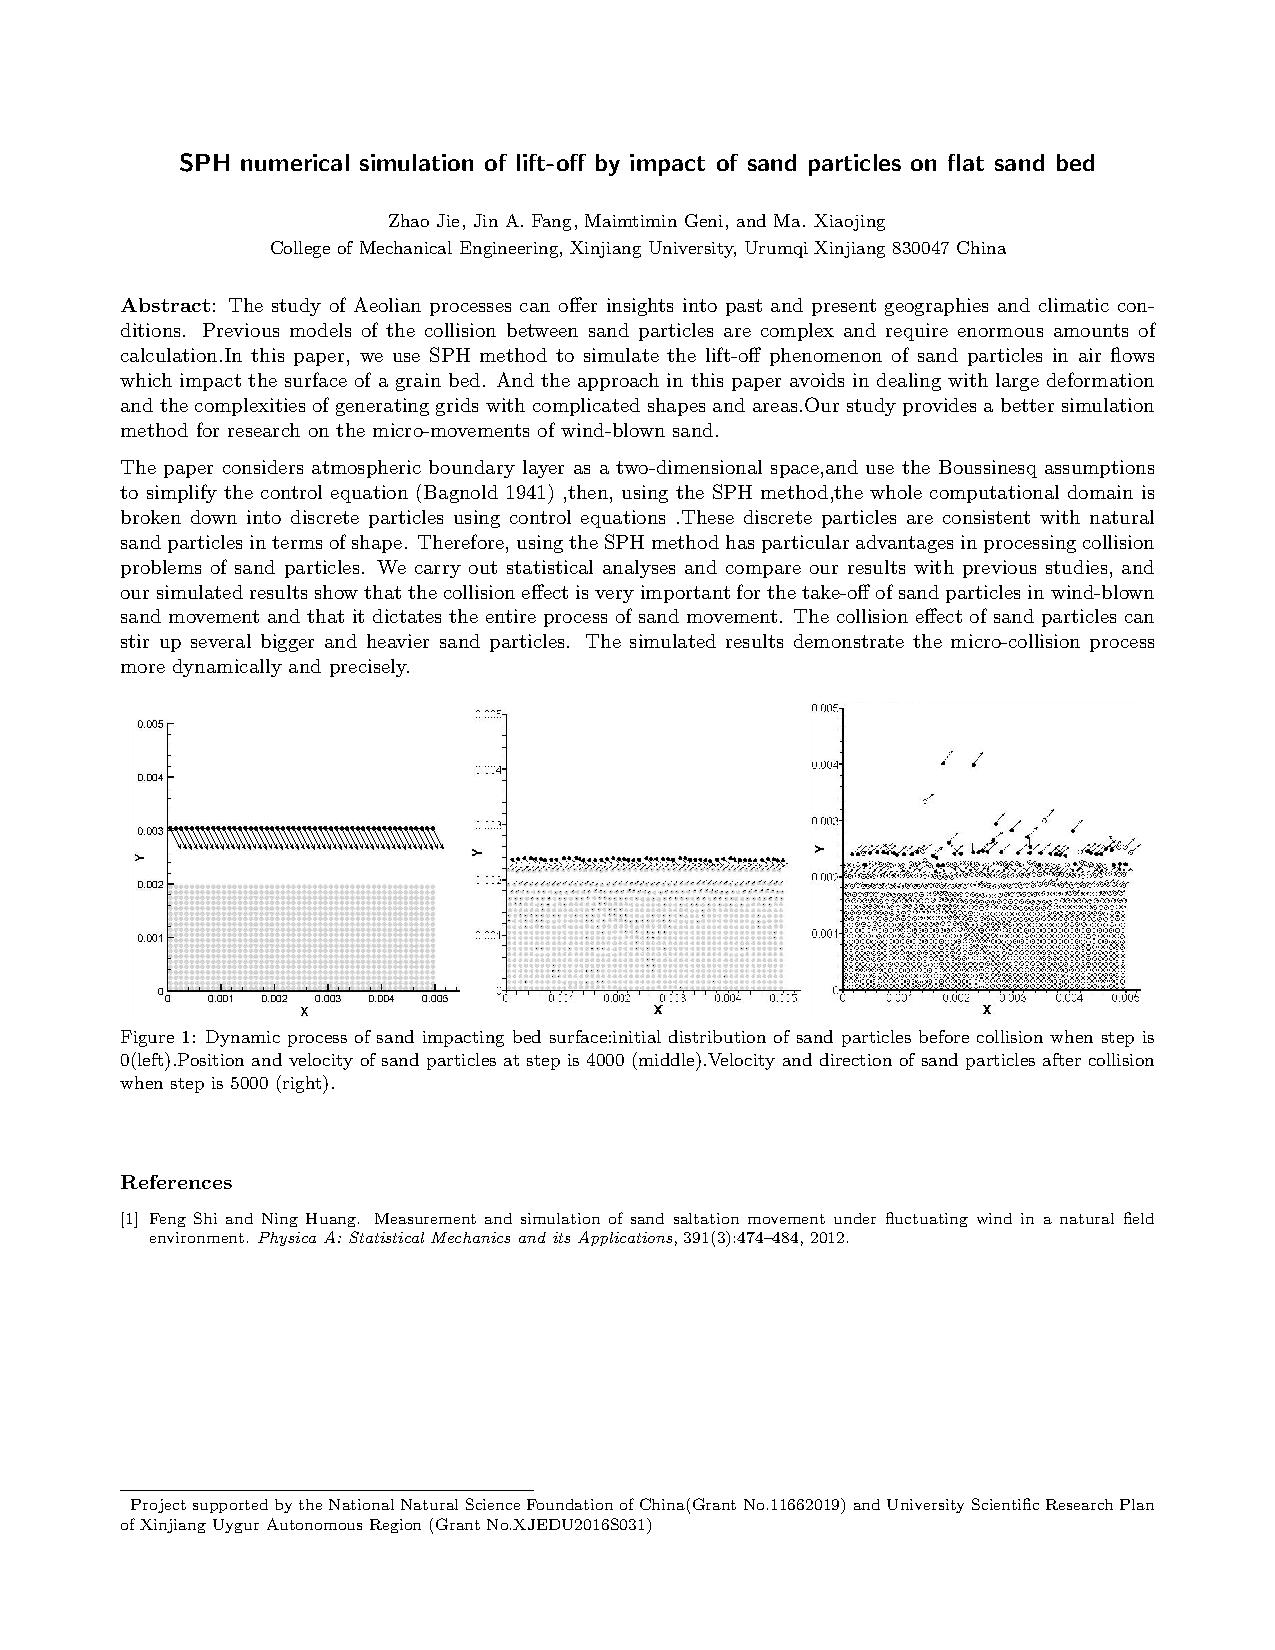
\includepdf[pages=-,pagecommand={\pagestyle{fancy}\label{4.4}},addtotoc={  
     1,subsection,1,SPH numerical simulation of lift-off by impact of sand particles on flat sand bed,p1}]{abstract/pdfs/44.pdf}

%\section{Session 5: Geotechnical  Applications}
%5.1: 4
%5.2: 5
%5.3: 6
%5.4: 33

\rhead{Session 5}
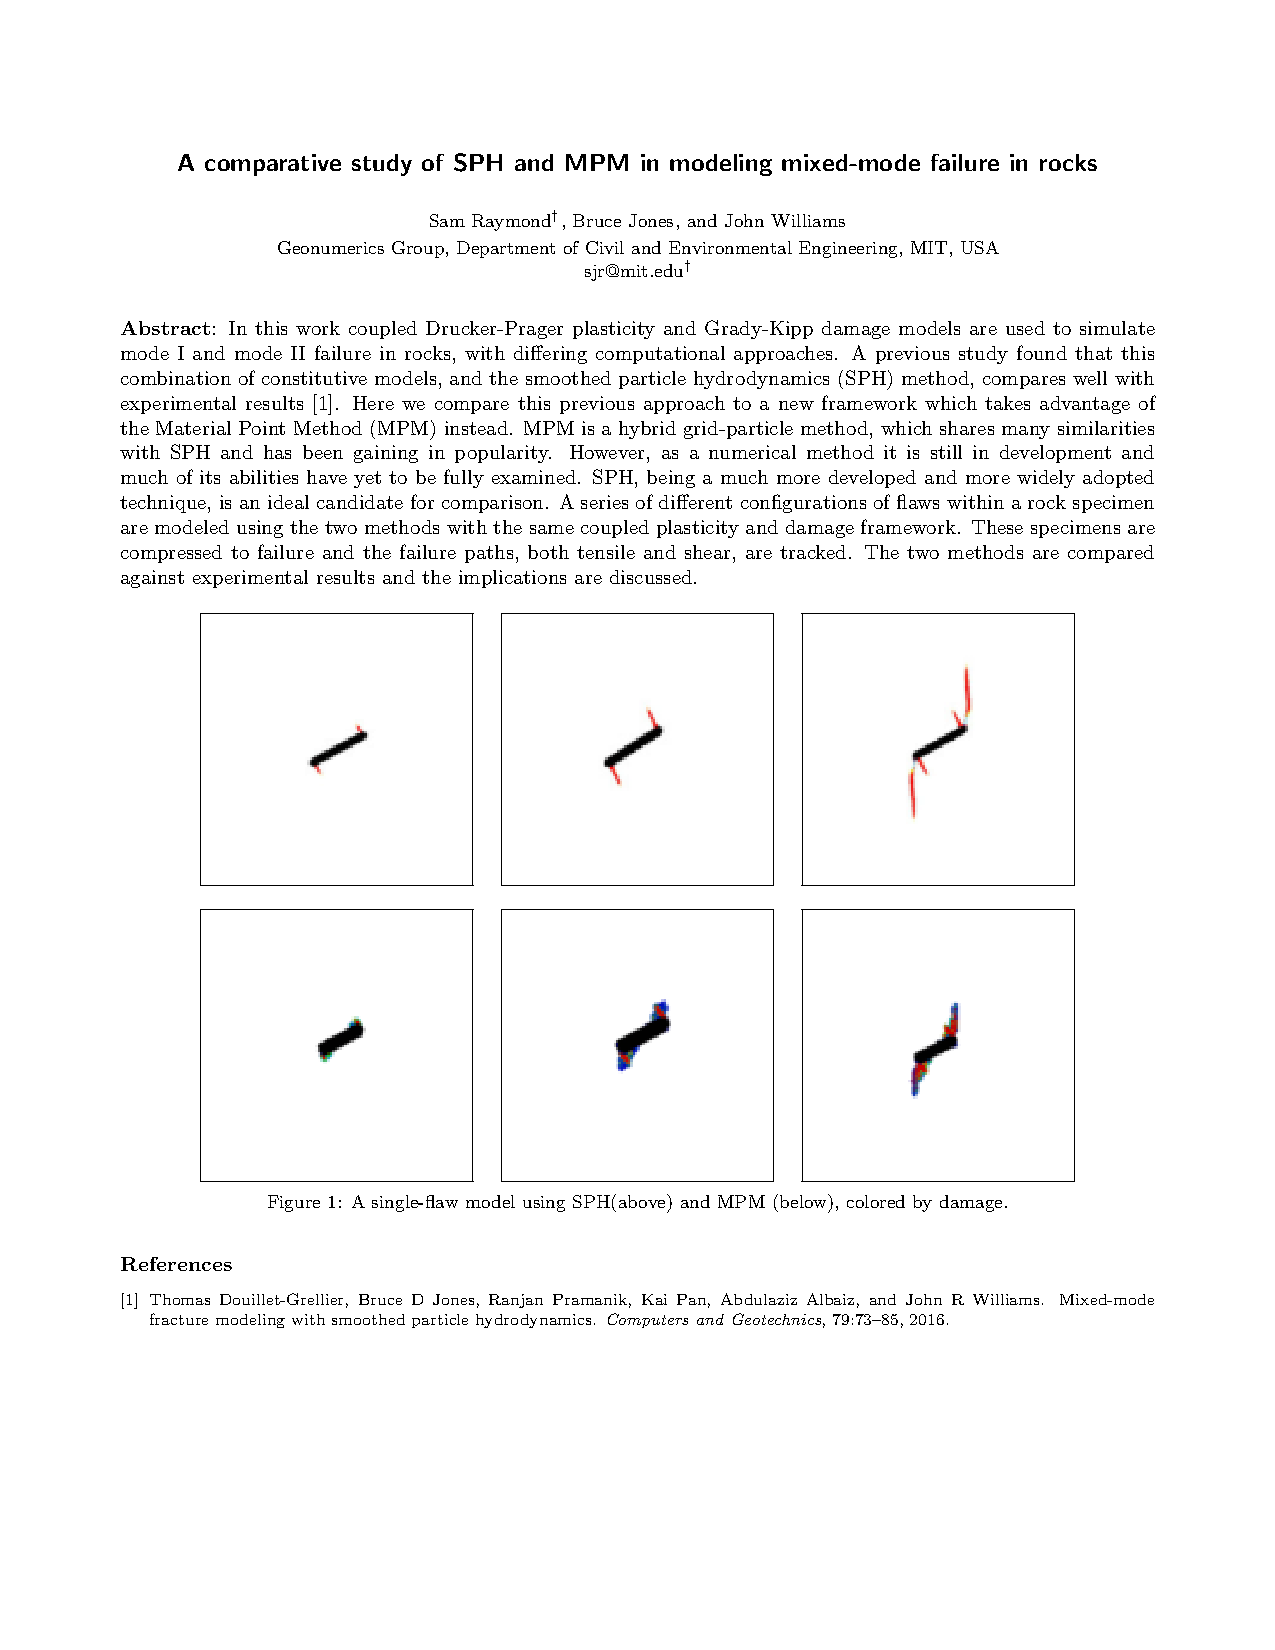
\includepdf[pages=-,pagecommand={\pagestyle{fancy}\label{5.1}},addtotoc={
     1,section,1,{~~~~~~~~Geotechnical Applications},p1,   
     1,subsection,1,A comparative study of SPH and MPM in modeling mixed-mode failure in rocks,p1}]{abstract/pdfs/4.pdf}
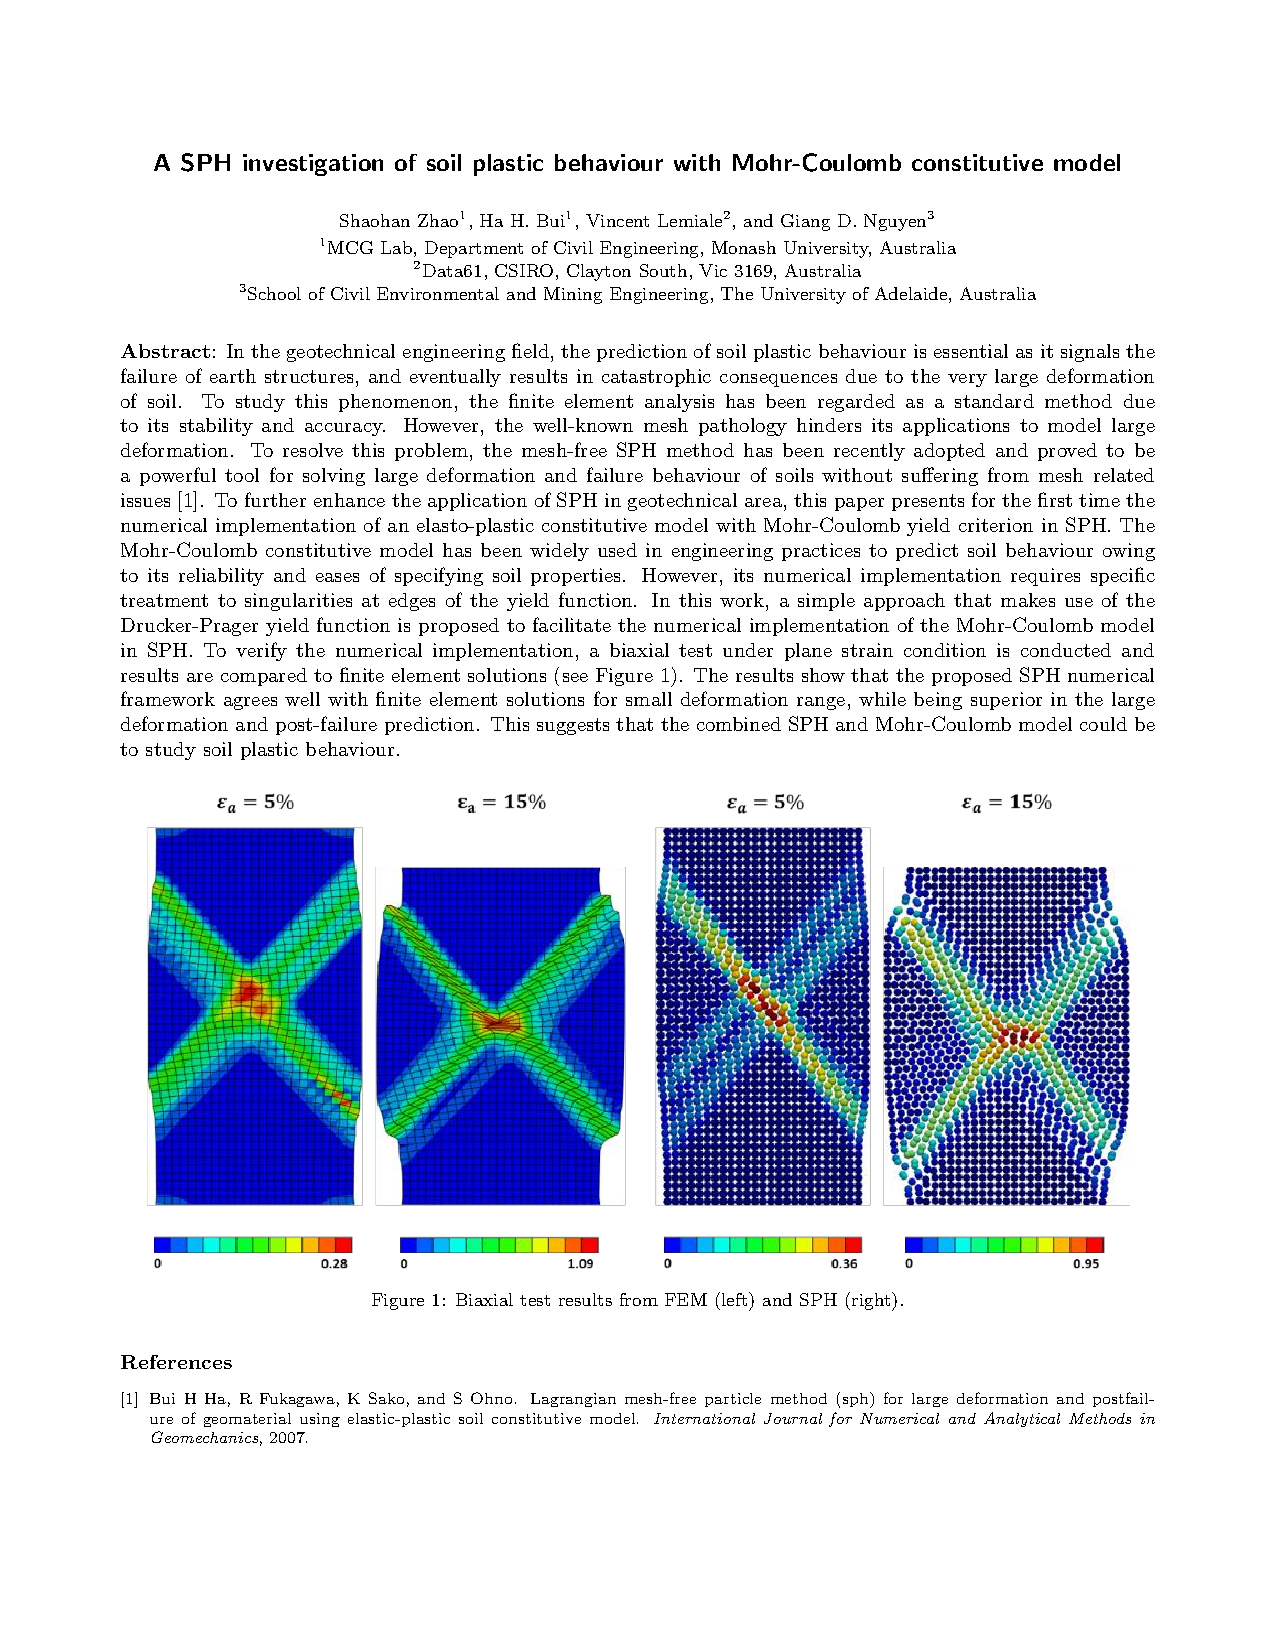
\includepdf[pages=-,pagecommand={\pagestyle{fancy}\label{5.2}},addtotoc={  
     1,subsection,1,A SPH investigation of soil plastic behaviour with Mohr-Coulomb constitutive model,p1}]{abstract/pdfs/5.pdf}
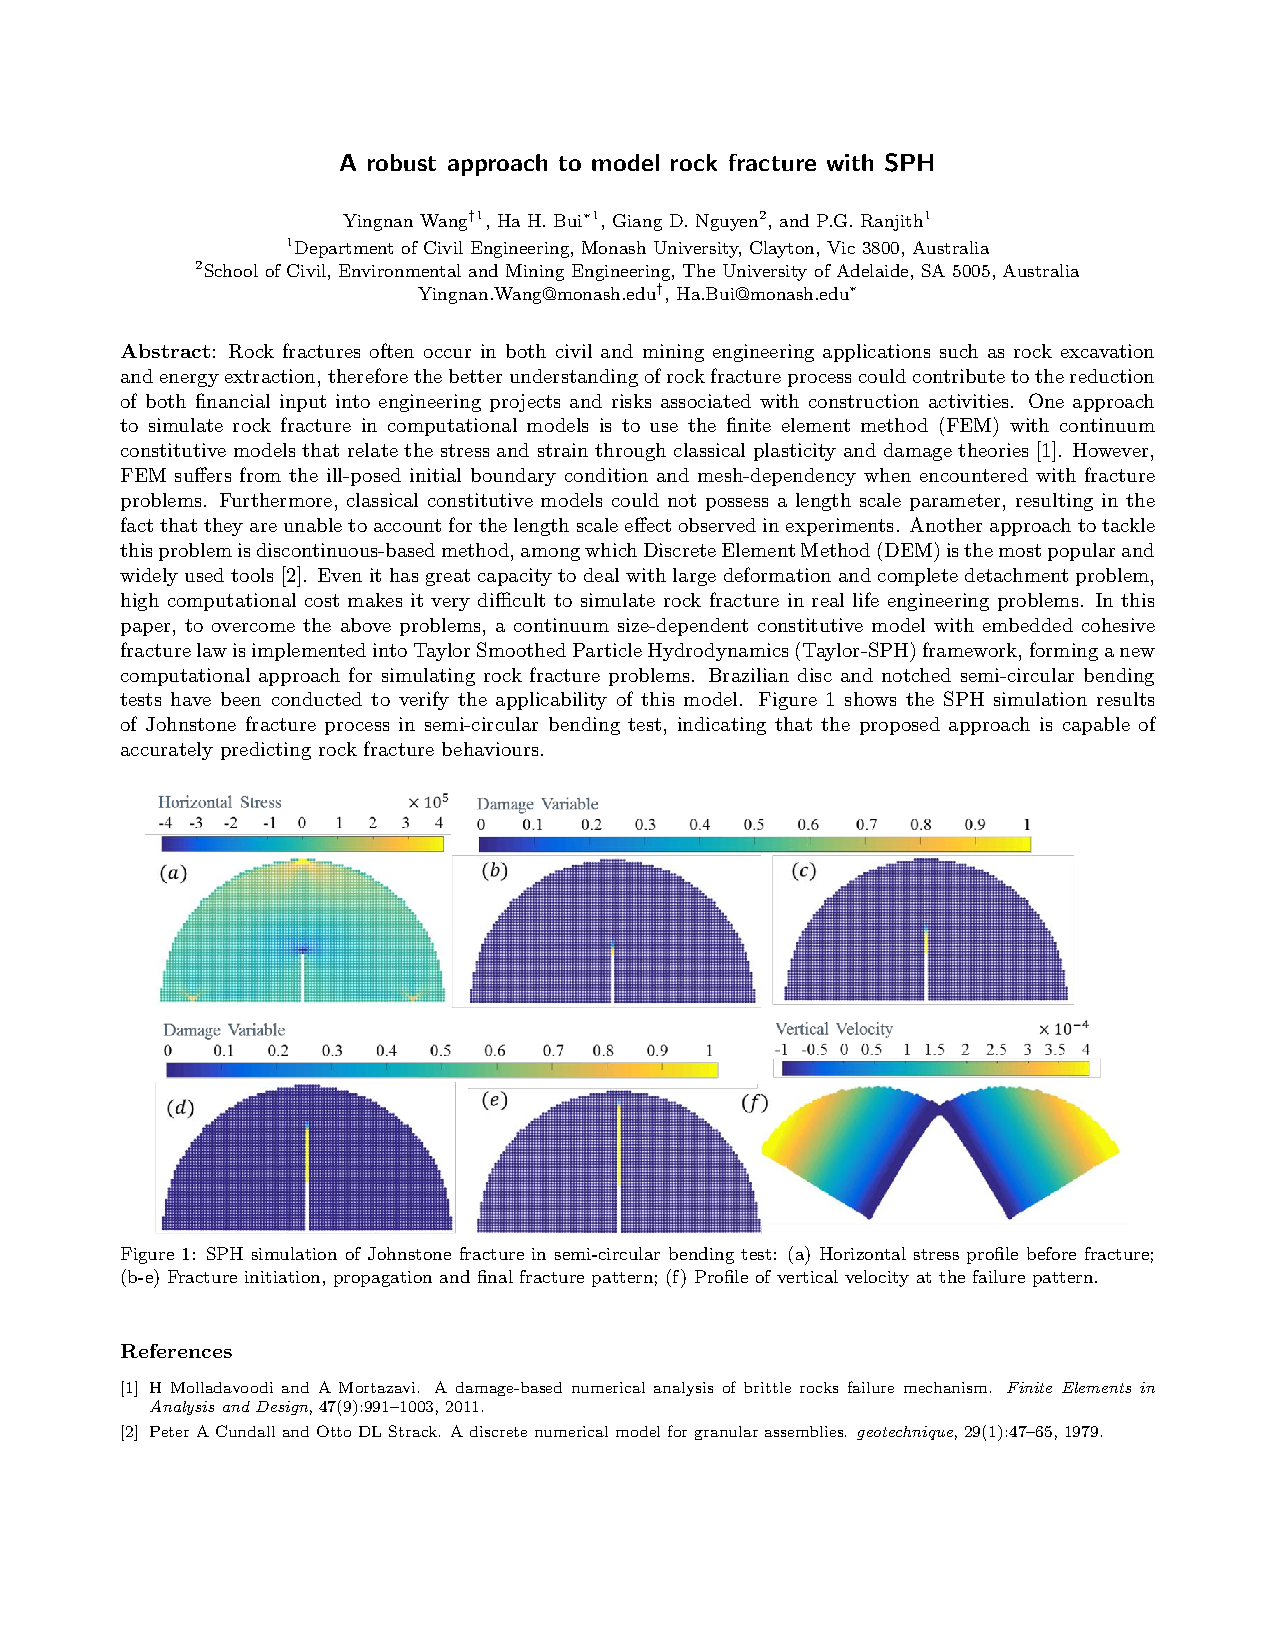
\includepdf[pages=-,pagecommand={\pagestyle{fancy}\label{5.3}},addtotoc={  
     1,subsection,1,A robust approach to model rock fracture with SPH,p1}]{abstract/pdfs/6.pdf}
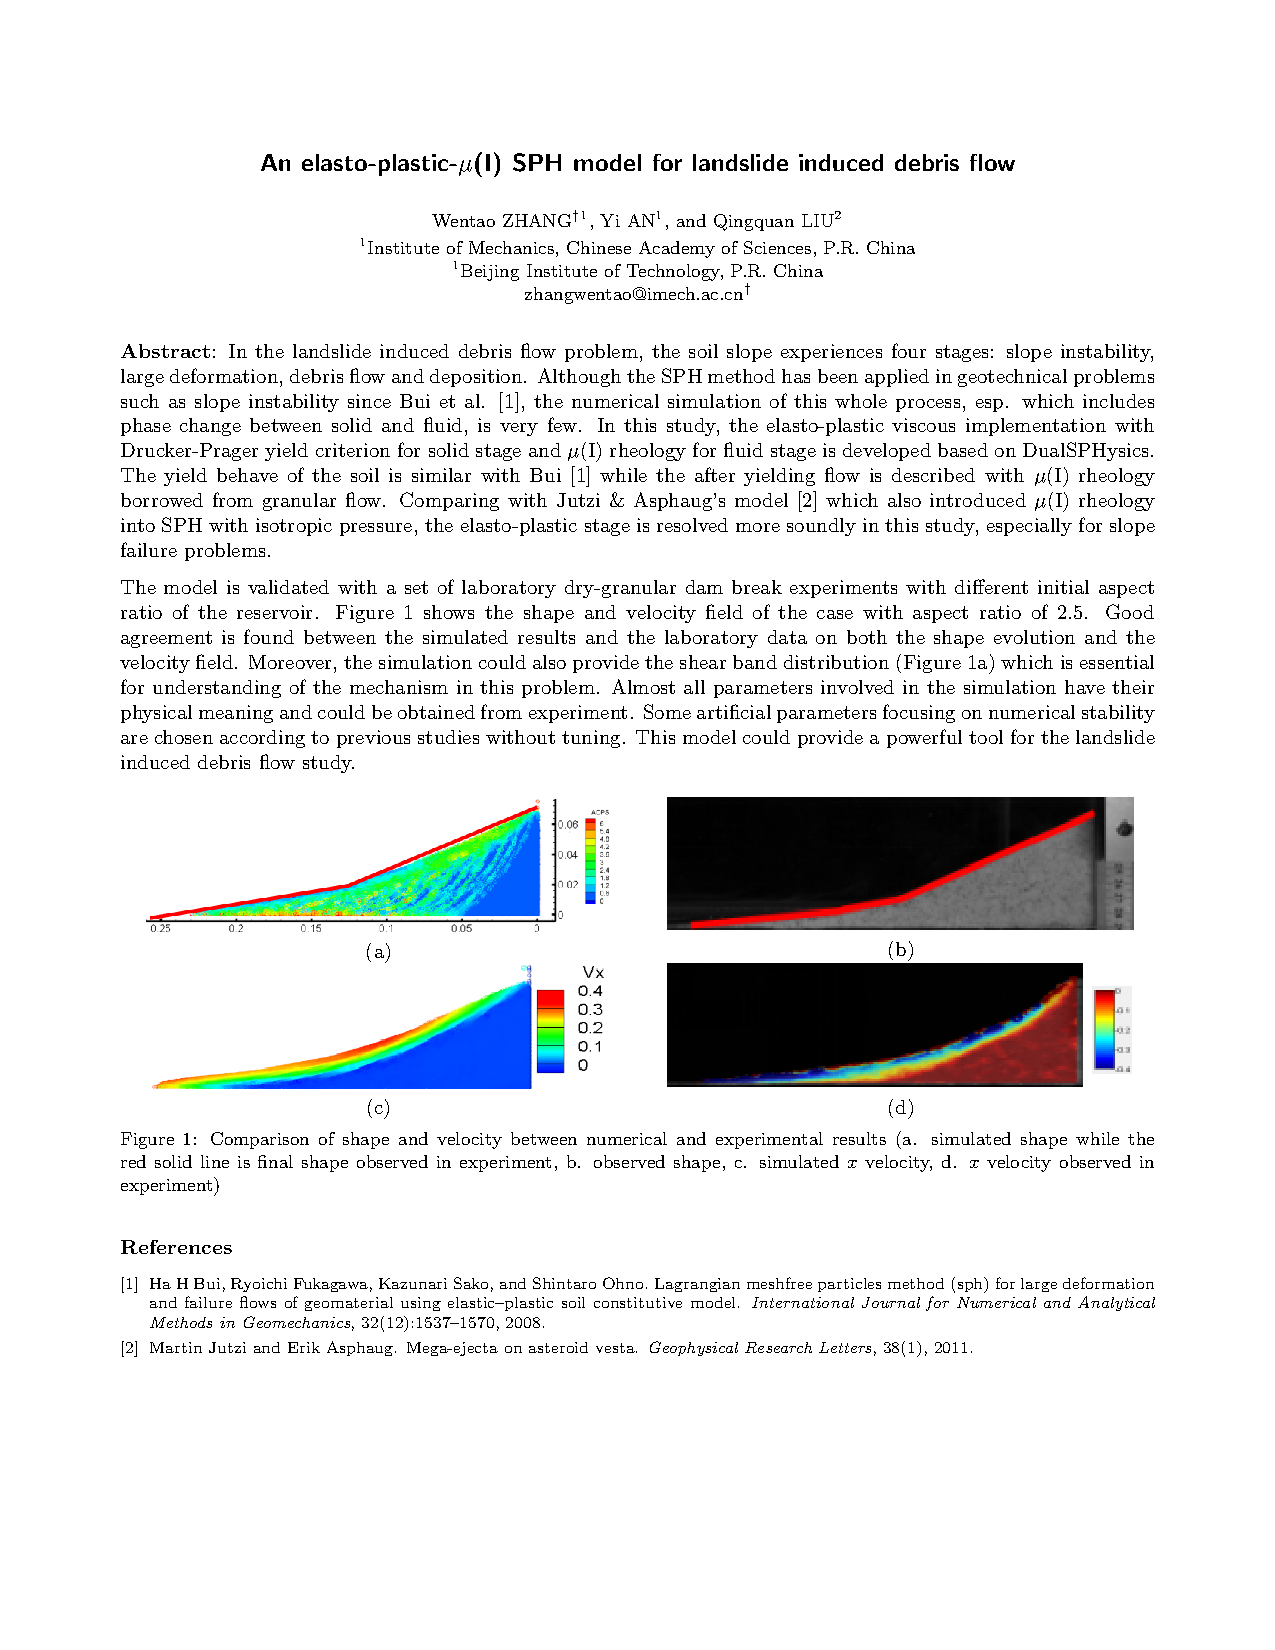
\includepdf[pages=-,pagecommand={\pagestyle{fancy}\label{5.4}},addtotoc={  
     1,subsection,1,An elasto-plastic-$\mu$(I) SPH model for landslide induced debris flow,p1}]{abstract/pdfs/33.pdf}



%\section{Session 6: Hydraulic Applications I}
%6.1: 10
%6.2: 48
%6.3: 46
%6.4: 55


\rhead{Session 6}
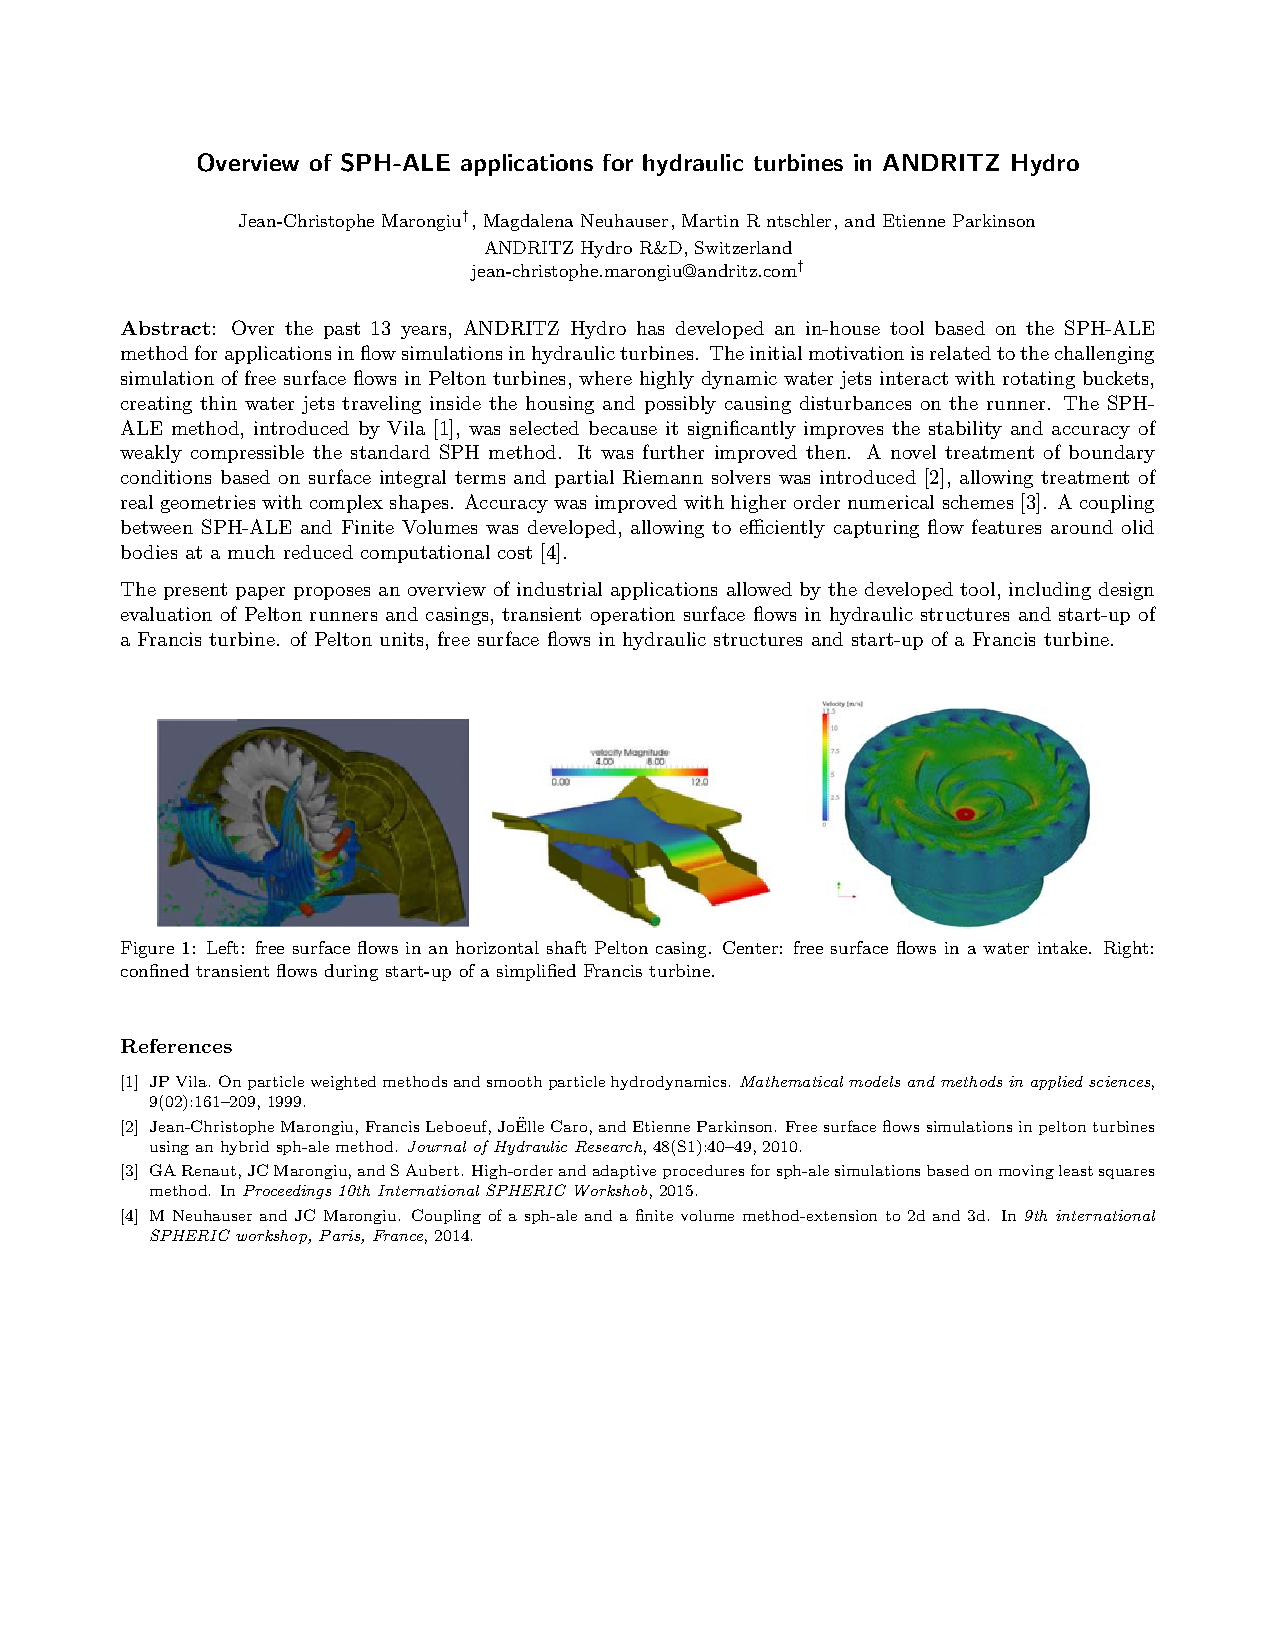
\includepdf[pages=-,pagecommand={\pagestyle{fancy}\label{6.1}},addtotoc={
     1,section,1,{~~~~~~~~Hydraulic Applications I},p1,   
     1,subsection,1,Overview of SPH-ALE applications for hydraulic turbines in ANDRITZ Hydro,p1}]{abstract/pdfs/10.pdf}
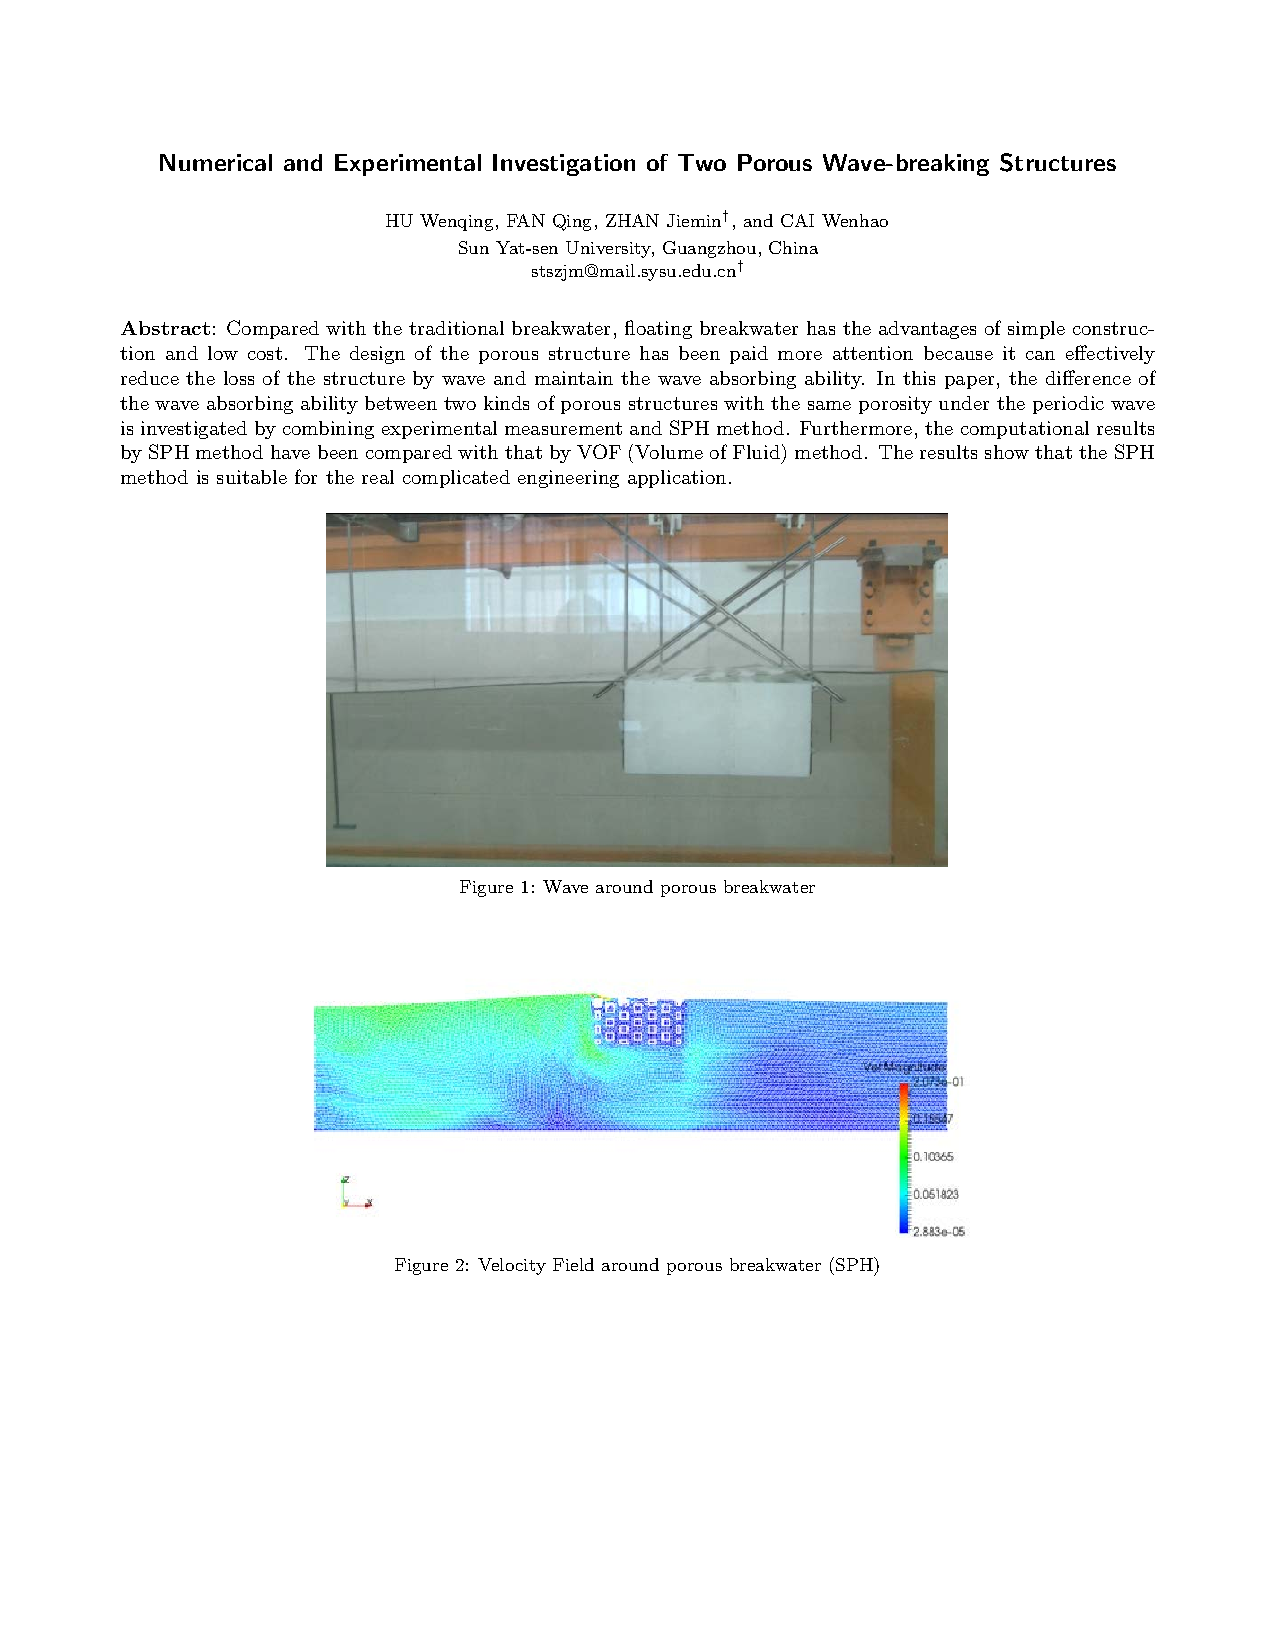
\includepdf[pages=-,pagecommand={\pagestyle{fancy}\label{6.2}},addtotoc={  
     1,subsection,1,Numerical and experimental investigation of two porous wave-breaking structures,p1}]{abstract/pdfs/48.pdf}
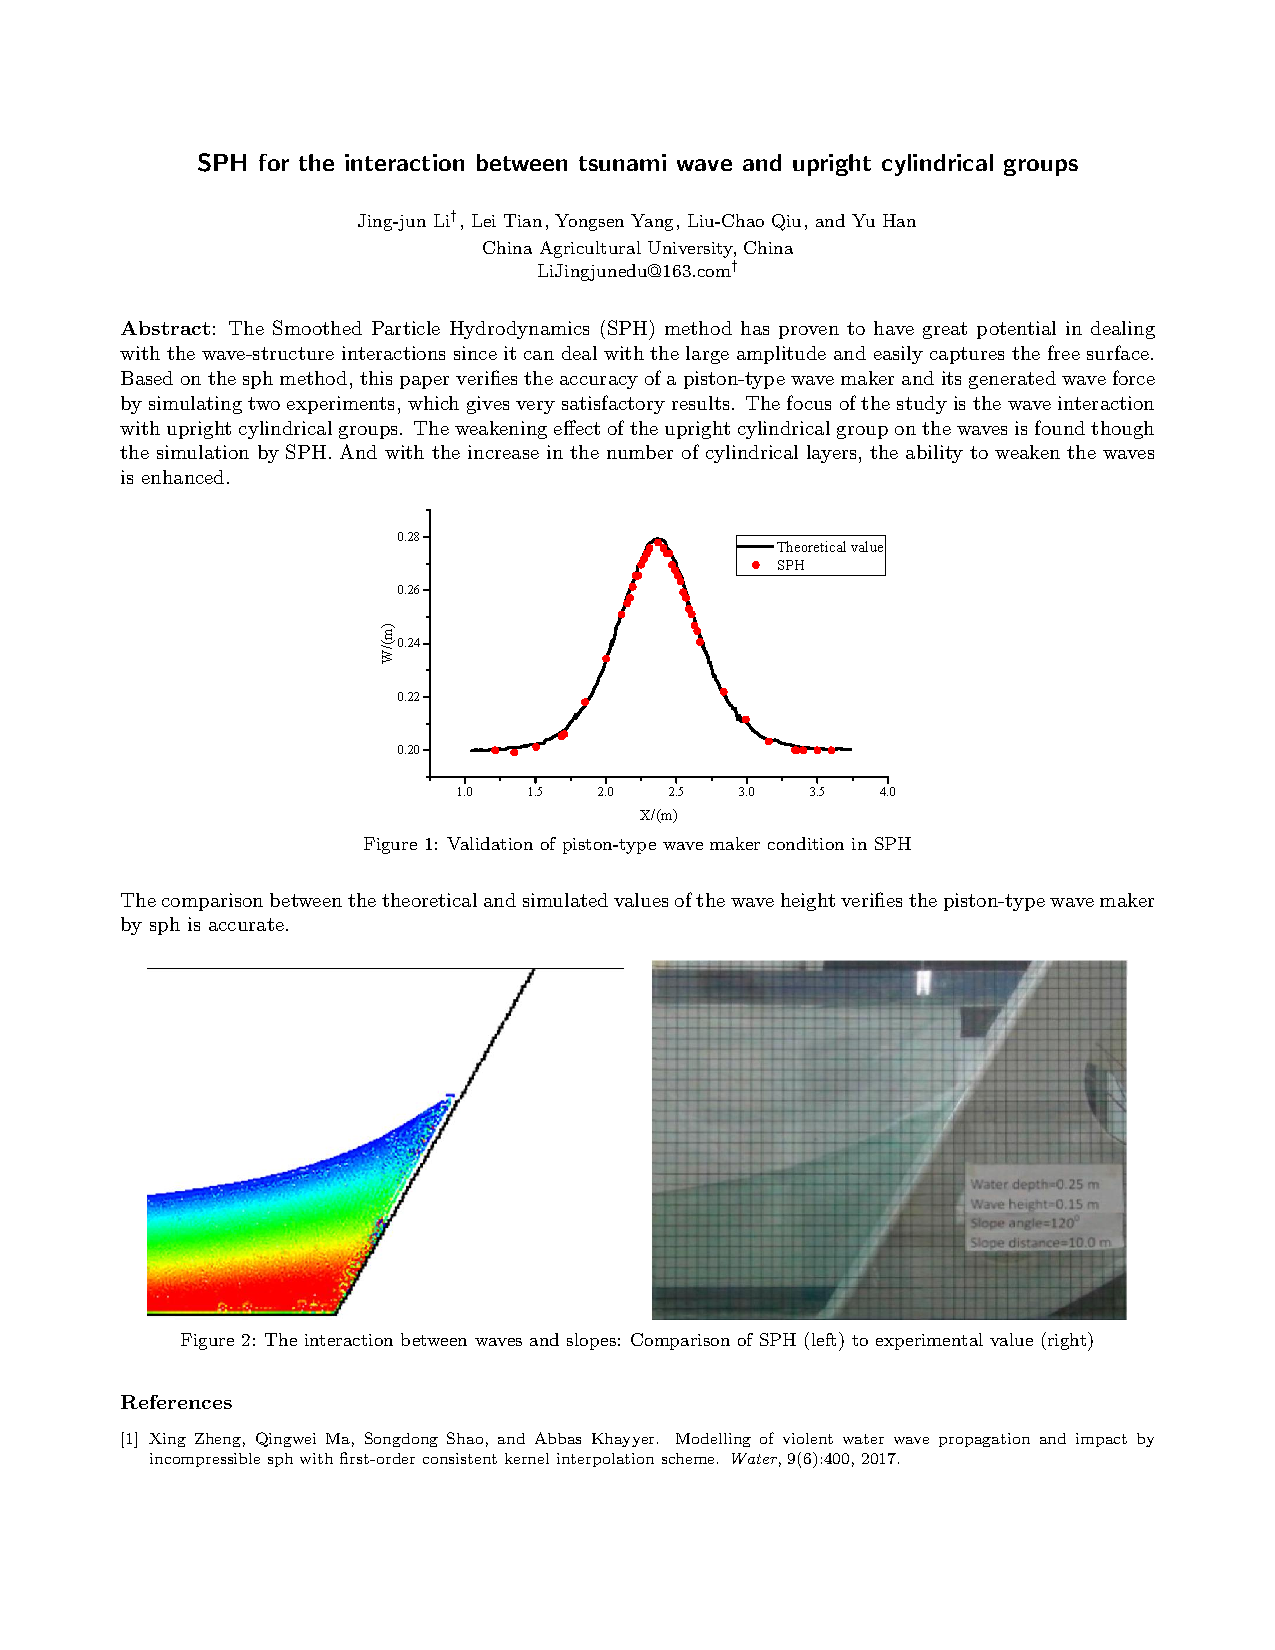
\includepdf[pages=-,pagecommand={\pagestyle{fancy}\label{6.3}},addtotoc={  
     1,subsection,1,SPH for the interaction between tsunami wave and upright cylindrical groups,p1}]{abstract/pdfs/46.pdf}
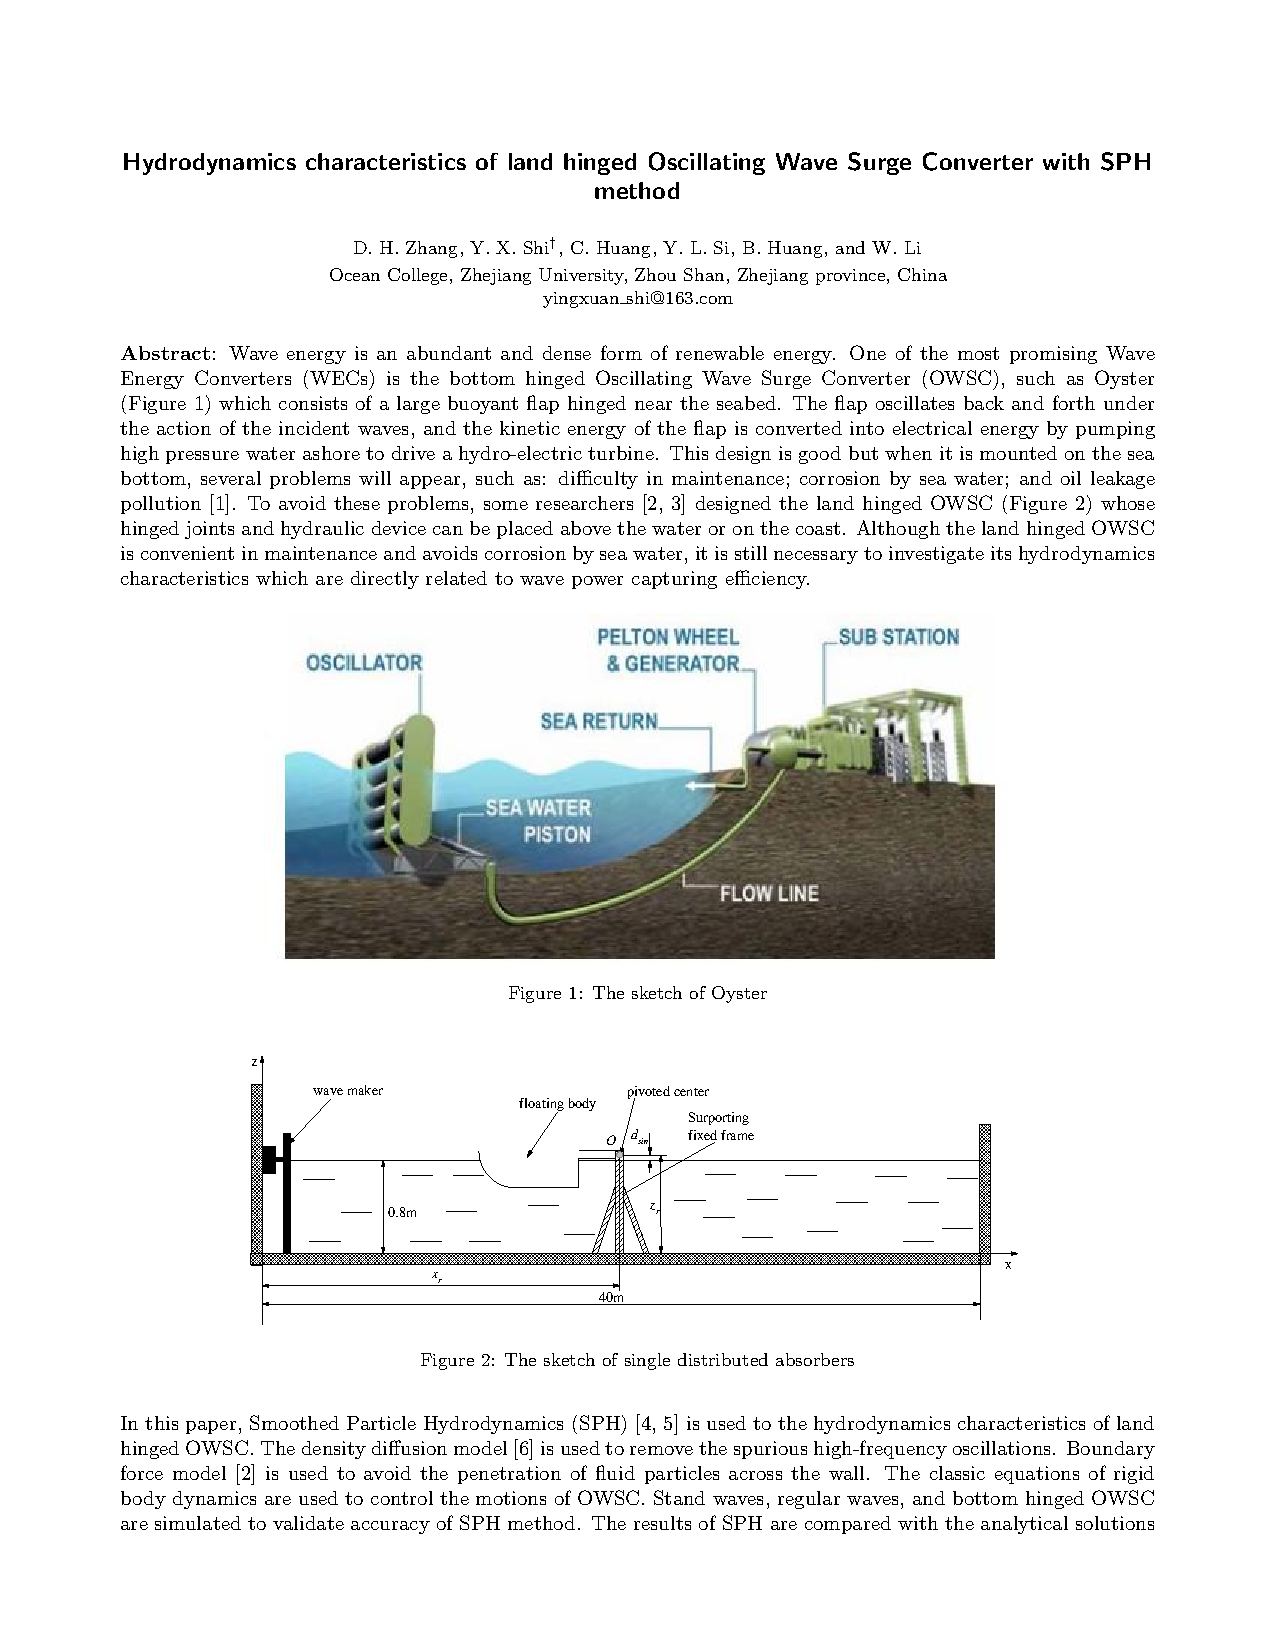
\includepdf[pages=-,pagecommand={\pagestyle{fancy}\label{6.4}},addtotoc={  
     1,subsection,1,Hydrodynamics characteristics of land hinged oscillating wave surge converter with SPH method,p1}]{abstract/pdfs/55.pdf}


%\section{Session 7: Adaptivity (variable resolution)}
%7.1: 15
%7.2: 29
%7.3: 12

\rhead{Session 7}
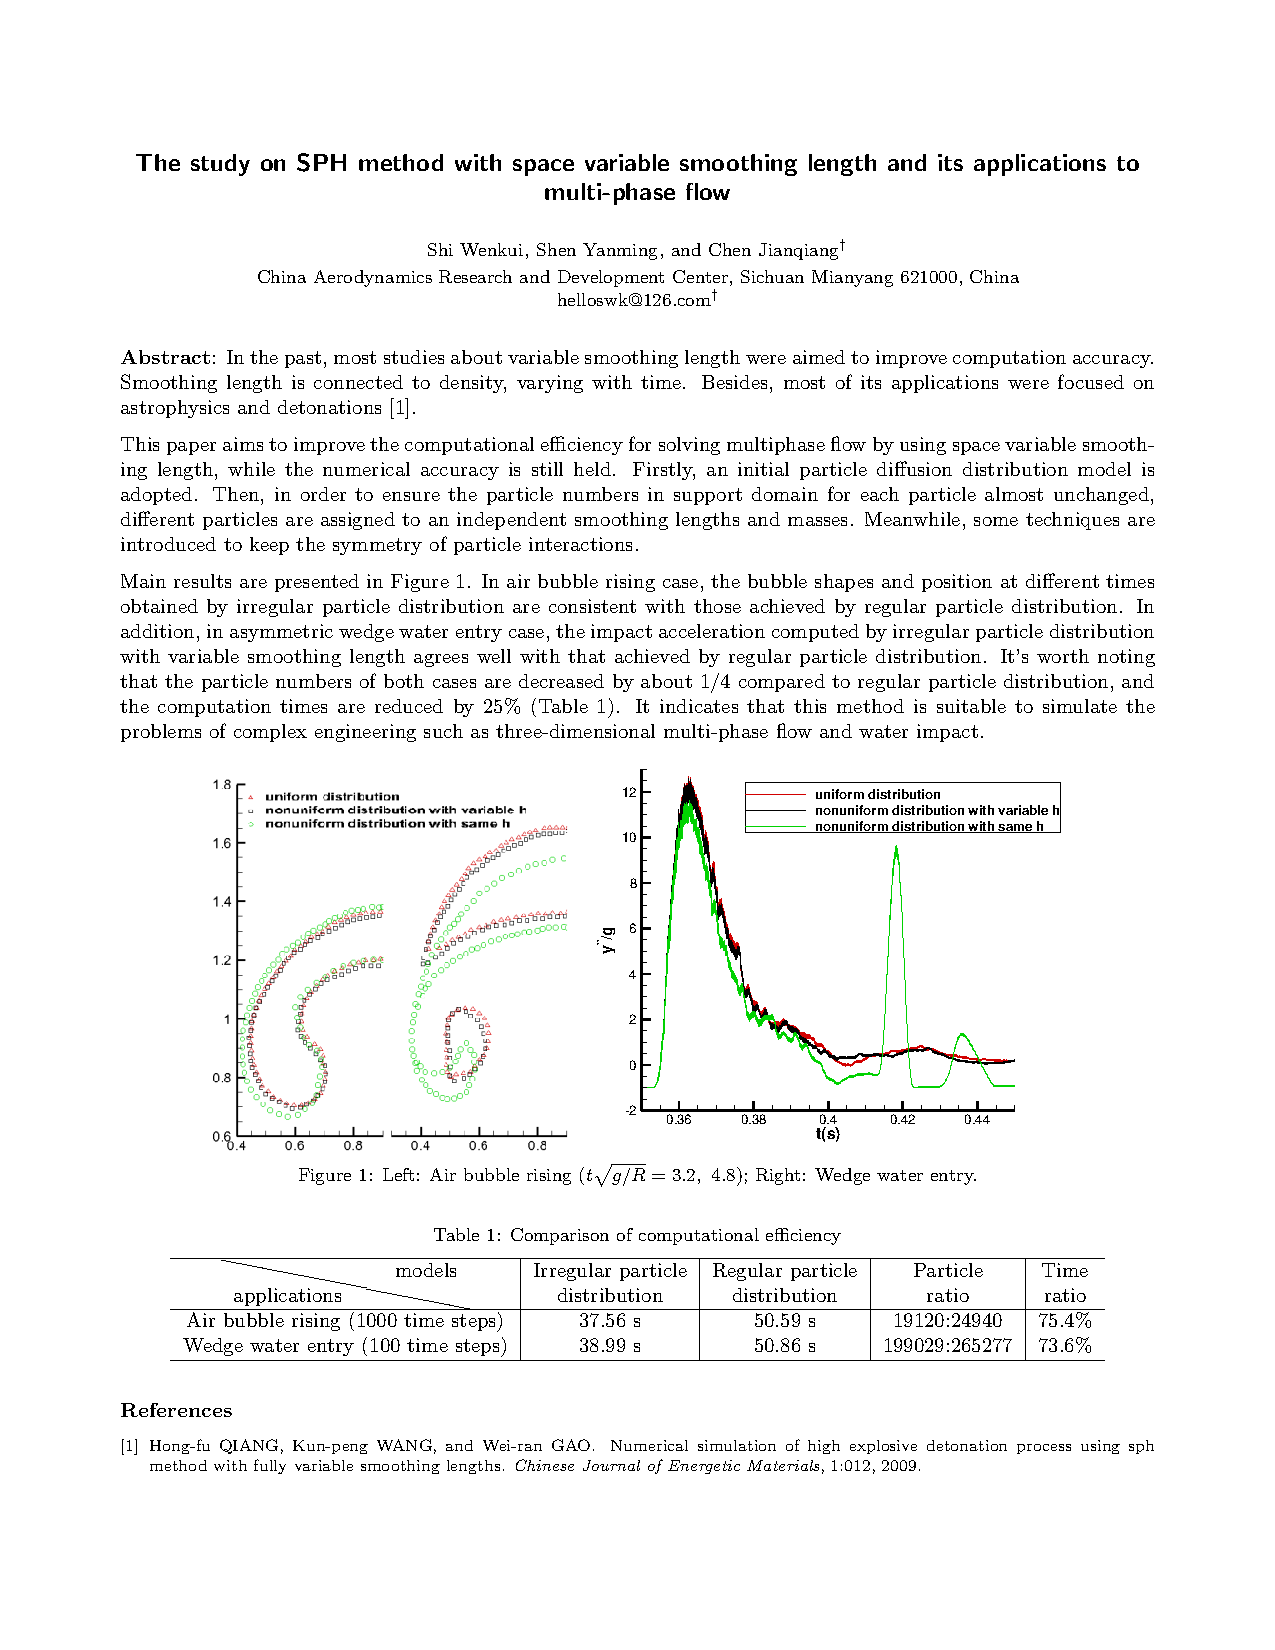
\includepdf[pages=-,pagecommand={\pagestyle{fancy}\label{7.1}},addtotoc={
     1,section,1,{~~~~~~~~Adaptivity (variable resolution)},p1,   
     1,subsection,1,The study on SPH method with space variable smoothing length and its applications to multi-phase flow,p1}]{abstract/pdfs/15.pdf}
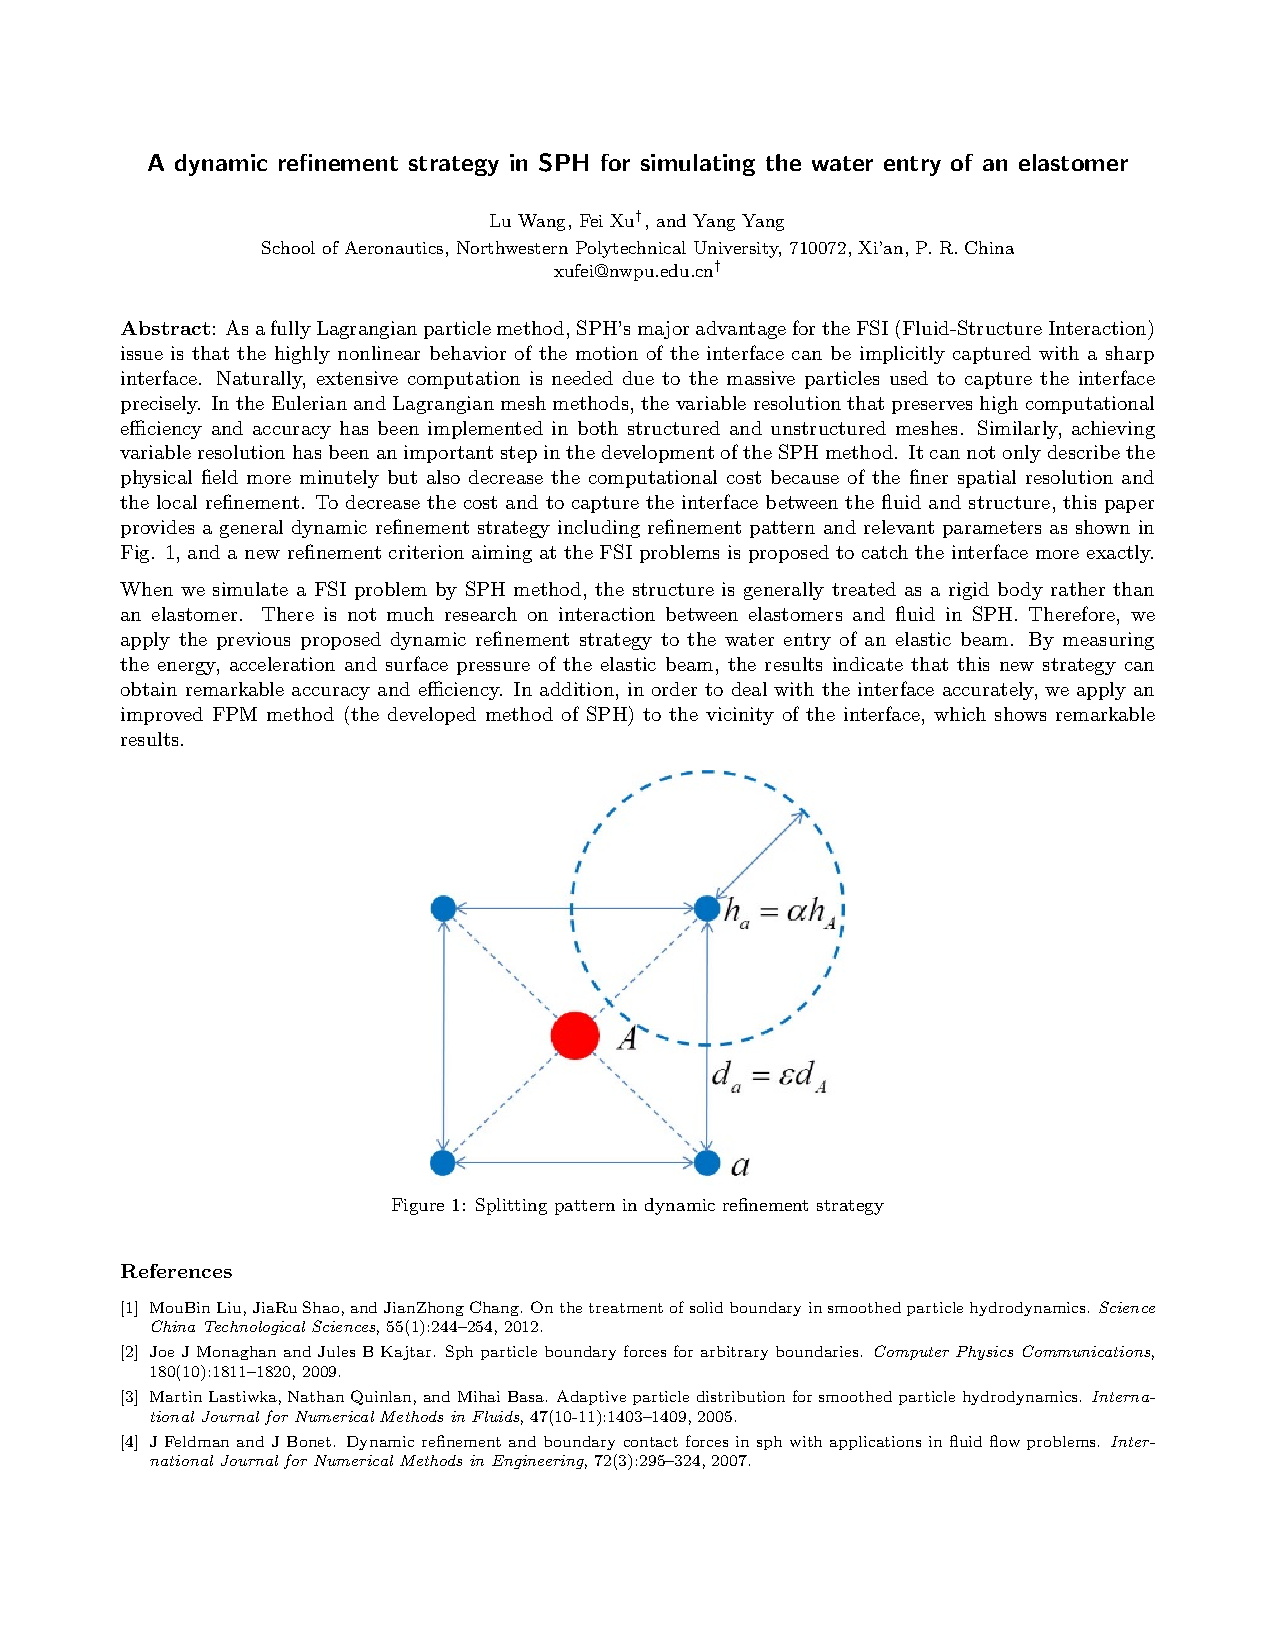
\includepdf[pages=-,pagecommand={\pagestyle{fancy}\label{7.2}},addtotoc={  
     1,subsection,1,A dynamic refinement strategy in SPH for simulating the water entry of an elastomer,p1}]{abstract/pdfs/29.pdf}
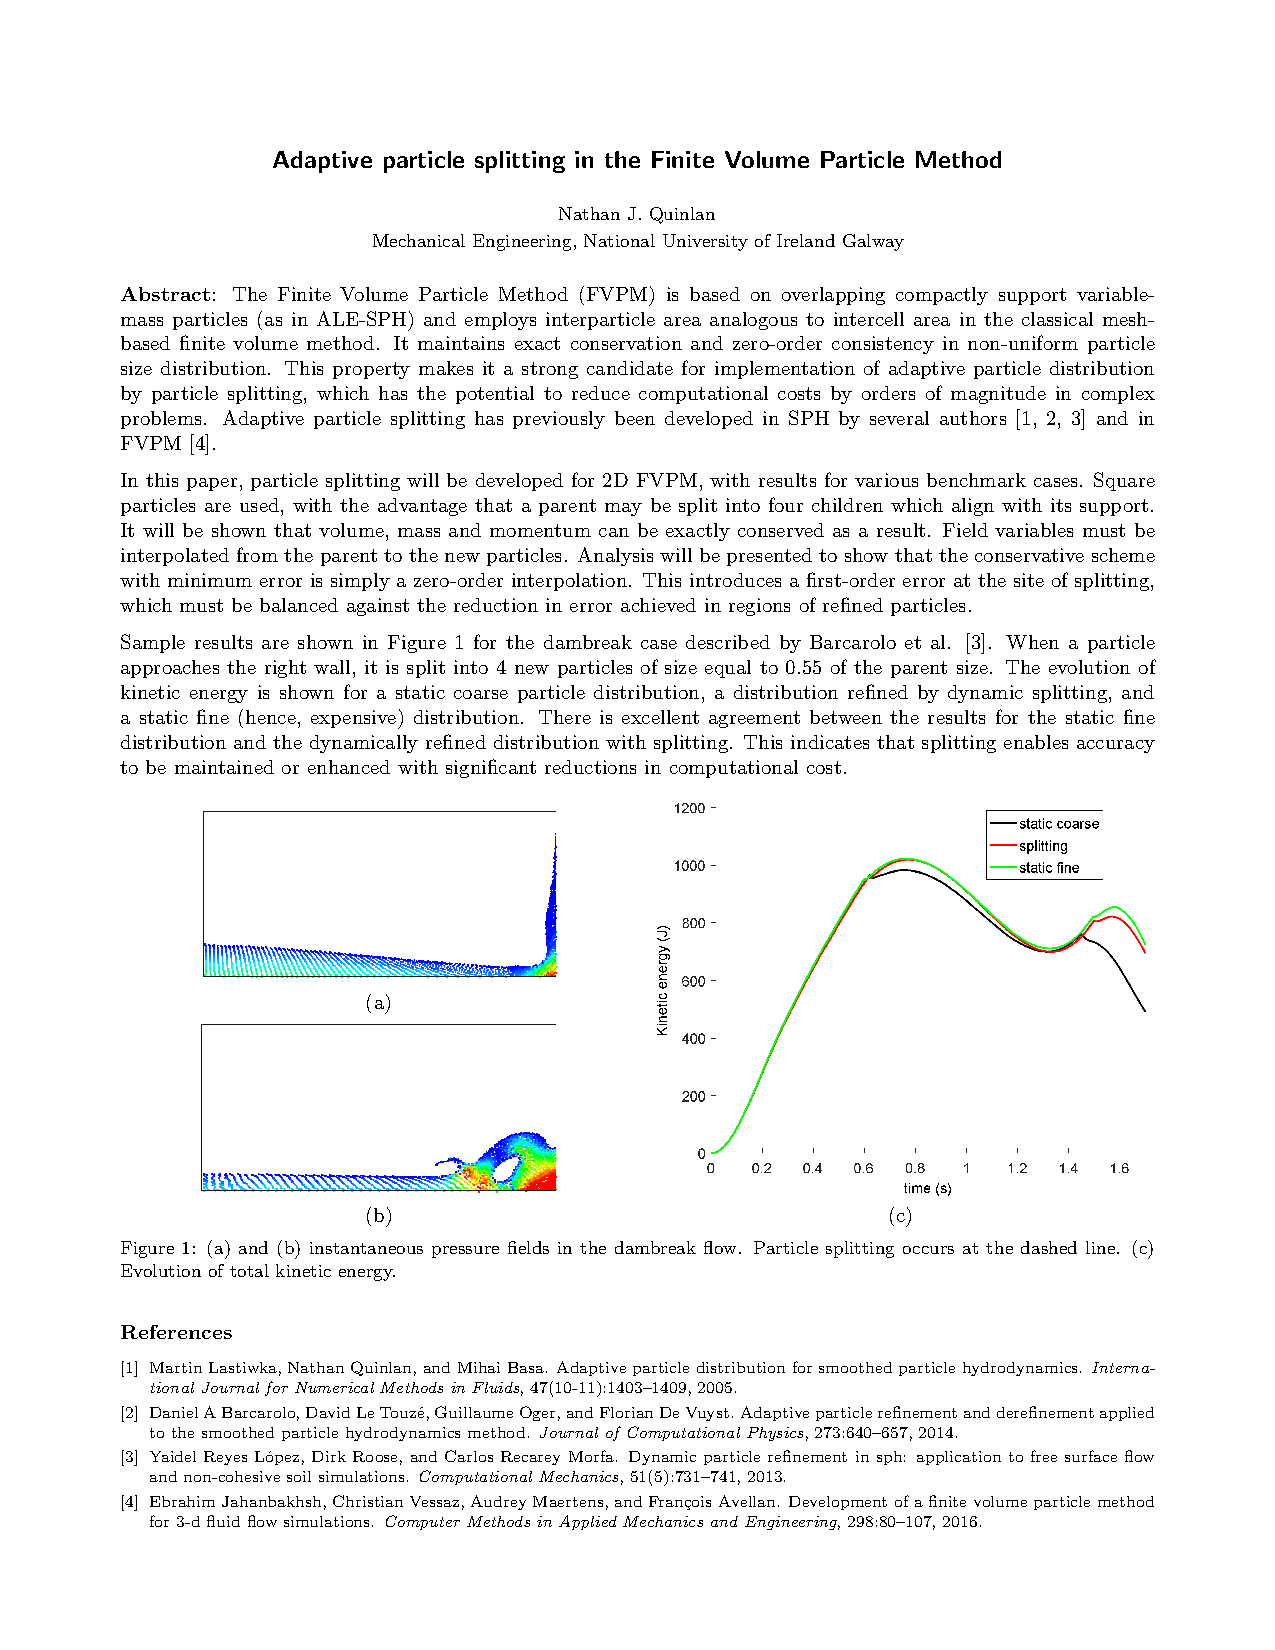
\includepdf[pages=-,pagecommand={\pagestyle{fancy}\label{7.3}},addtotoc={  
     1,subsection,1,Adaptive particle splitting in the finite volume particle method,p1}]{abstract/pdfs/12.pdf}



%\section{Session 8: New applications of SPH}
%8.1: 25
%8.2: 38
%8.3: 3
%8.4: 9

\rhead{Session 8}
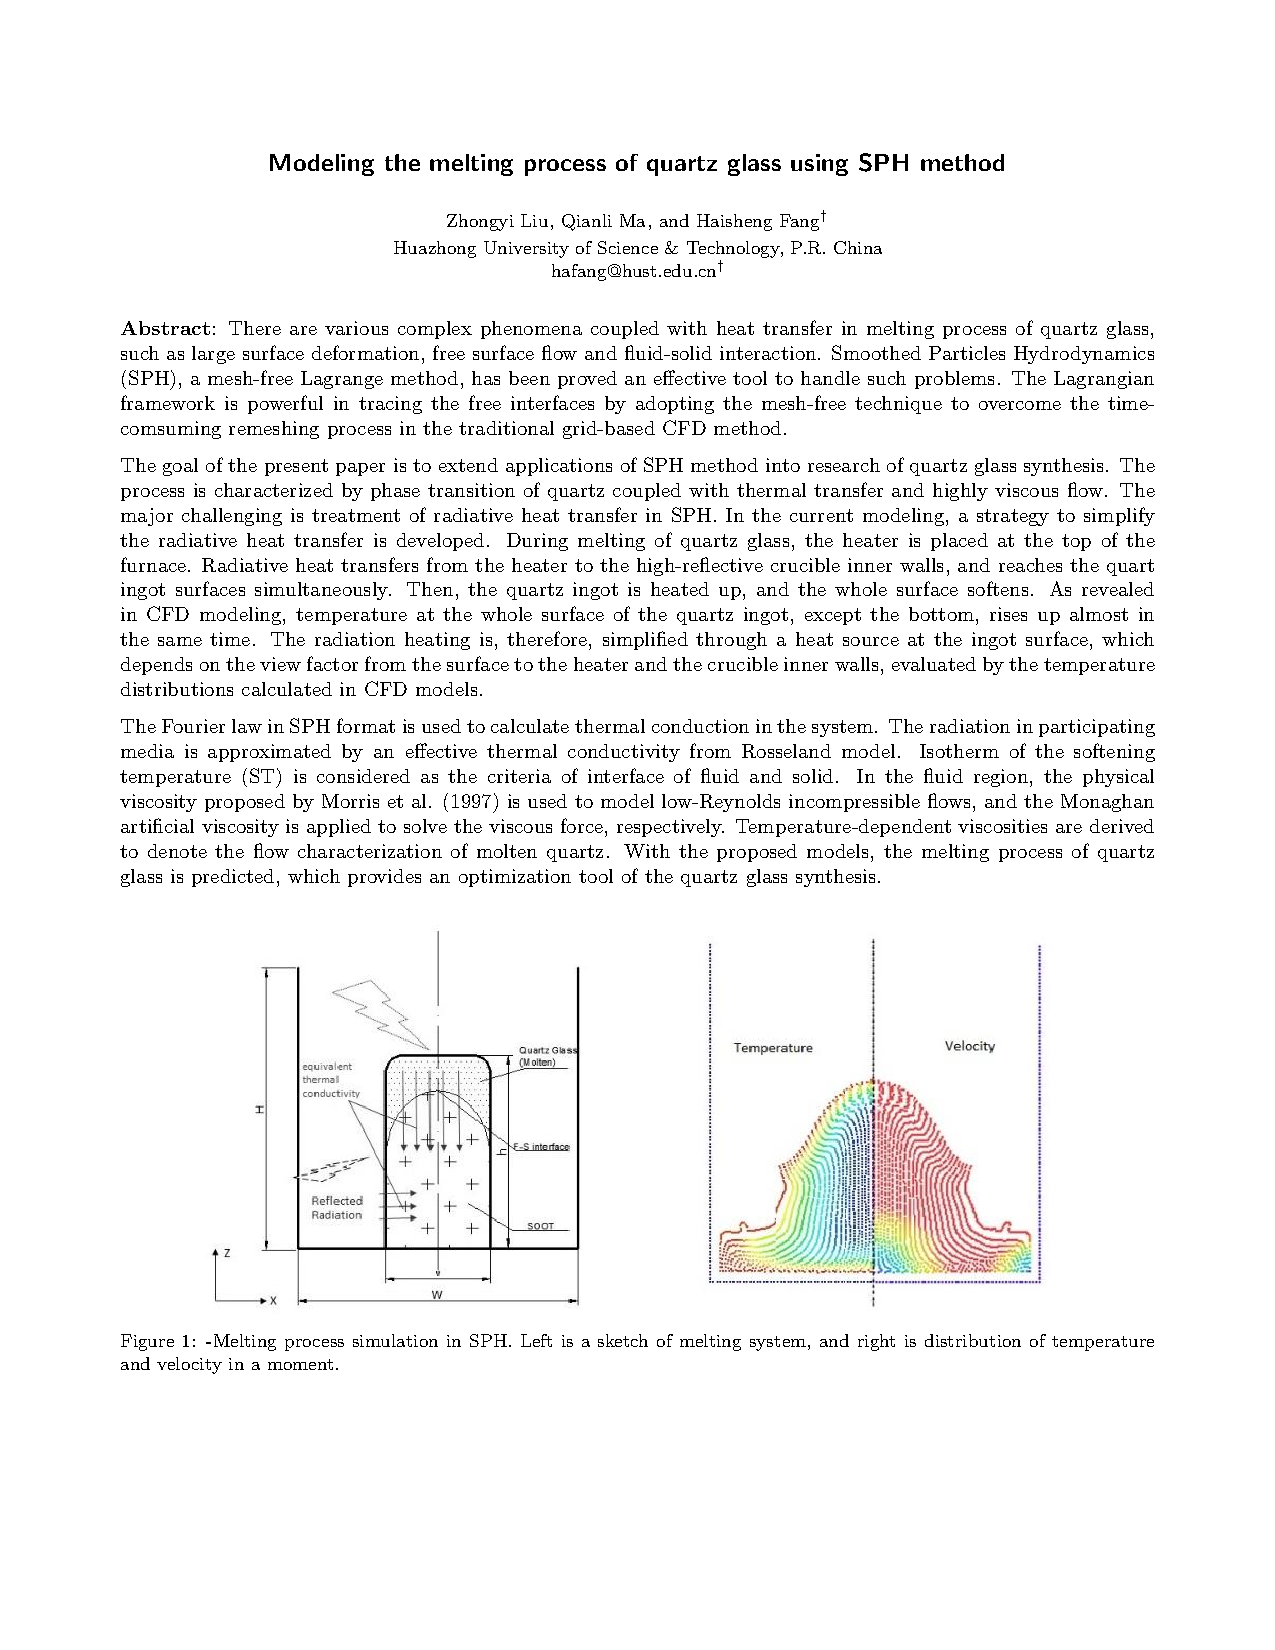
\includepdf[pages=-,pagecommand={\pagestyle{fancy}\label{8.1}},addtotoc={
     1,section,1,{~~~~~~~~New applications of SPH},p1,   
     1,subsection,1,Modeling the melting process of quartz glass using SPH method,p1}]{abstract/pdfs/25.pdf}
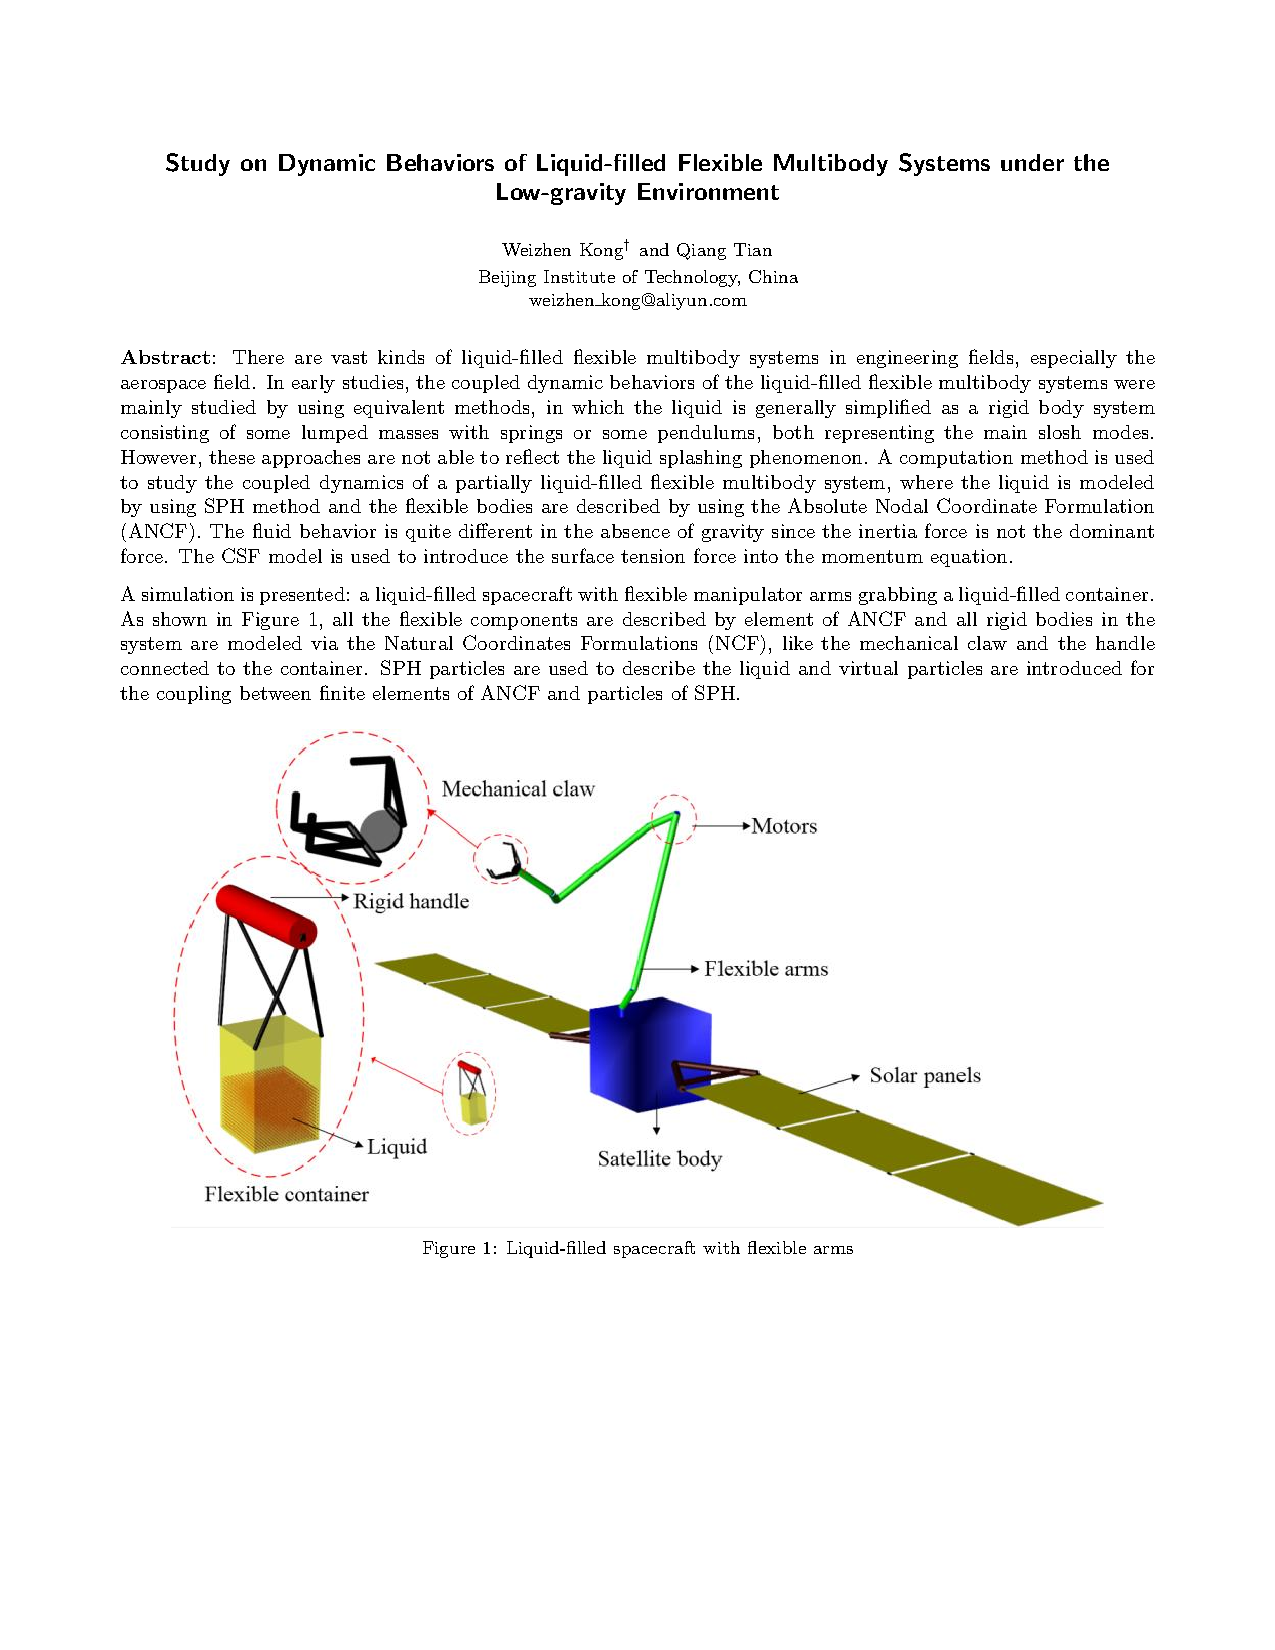
\includepdf[pages=-,pagecommand={\pagestyle{fancy}\label{8.2}},addtotoc={  
     1,subsection,1,Study on dynamic behaviors of liquid-filled flexible multibody systems under the low-gravity environment,p1}]{abstract/pdfs/38.pdf}
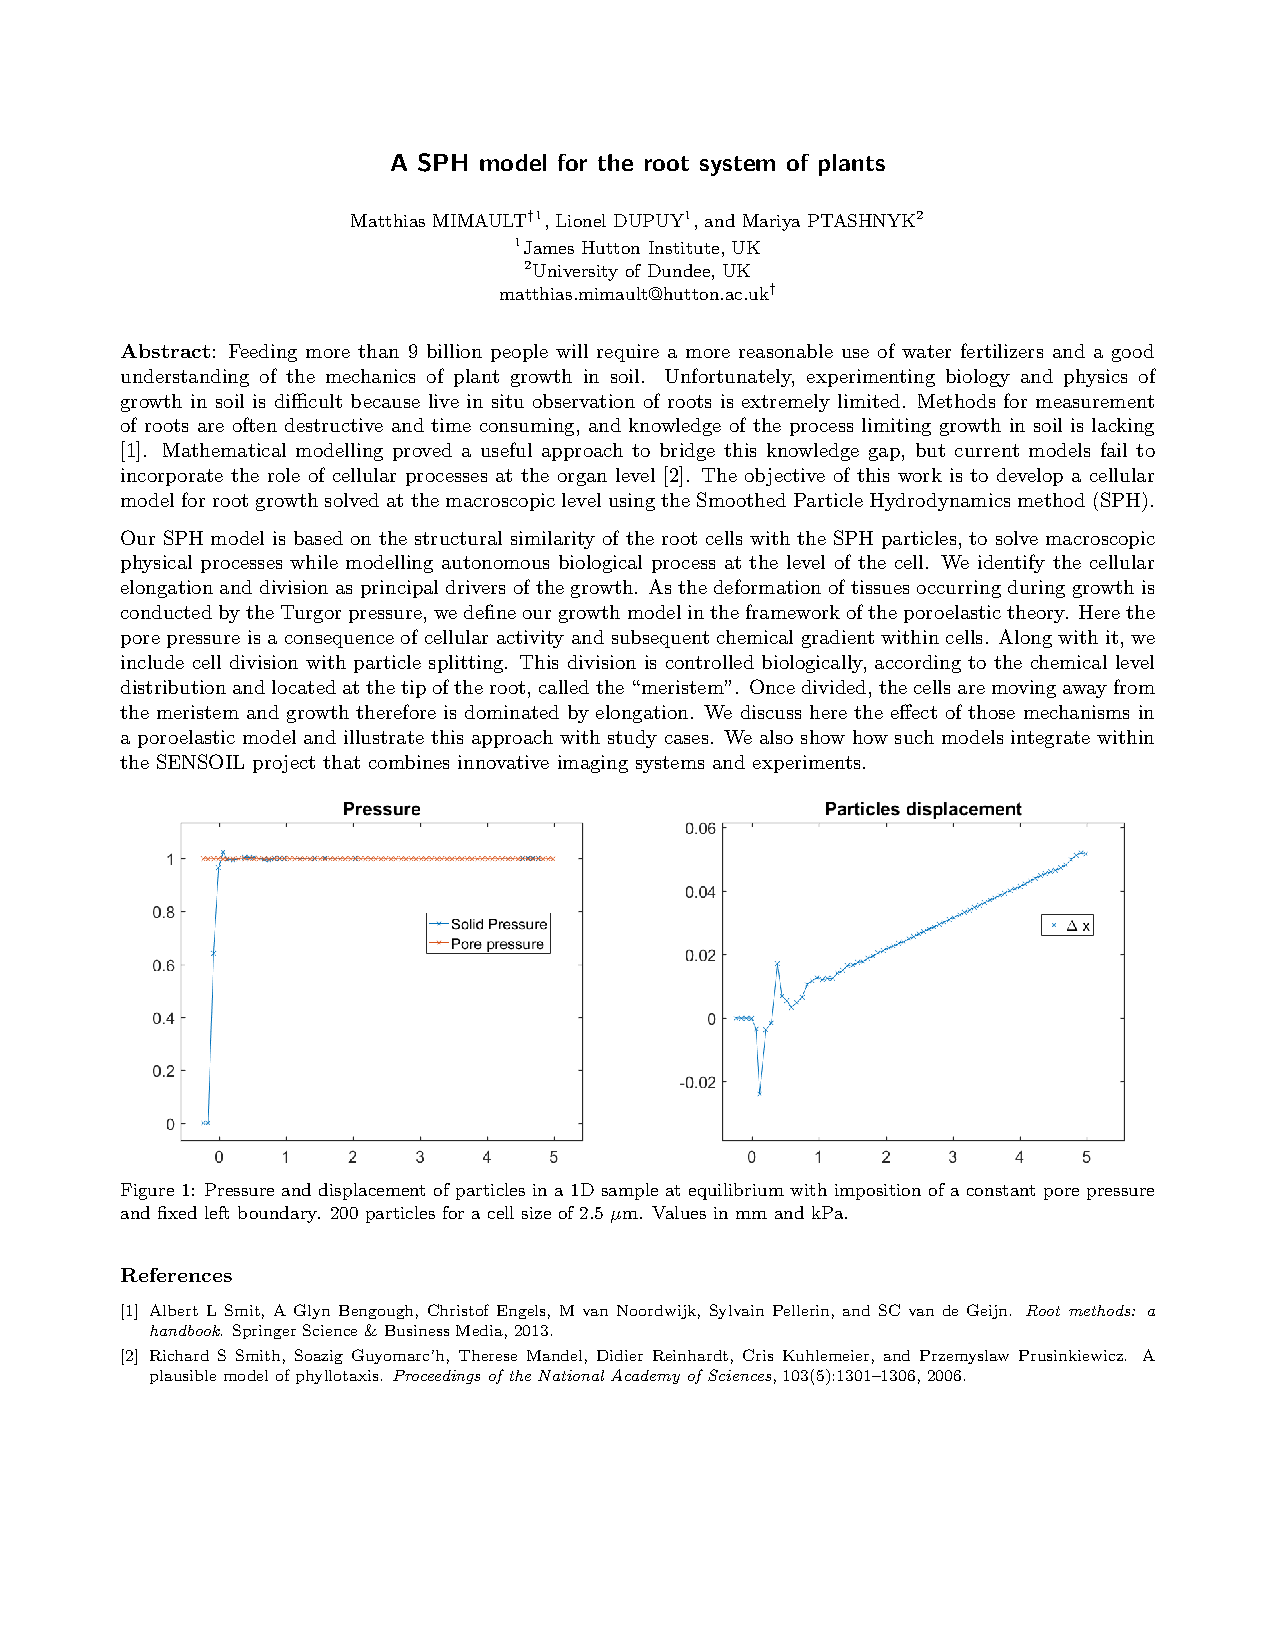
\includepdf[pages=-,pagecommand={\pagestyle{fancy}\label{8.3}},addtotoc={  
     1,subsection,1,A SPH model for the root system of plants,p1}]{abstract/pdfs/3.pdf}
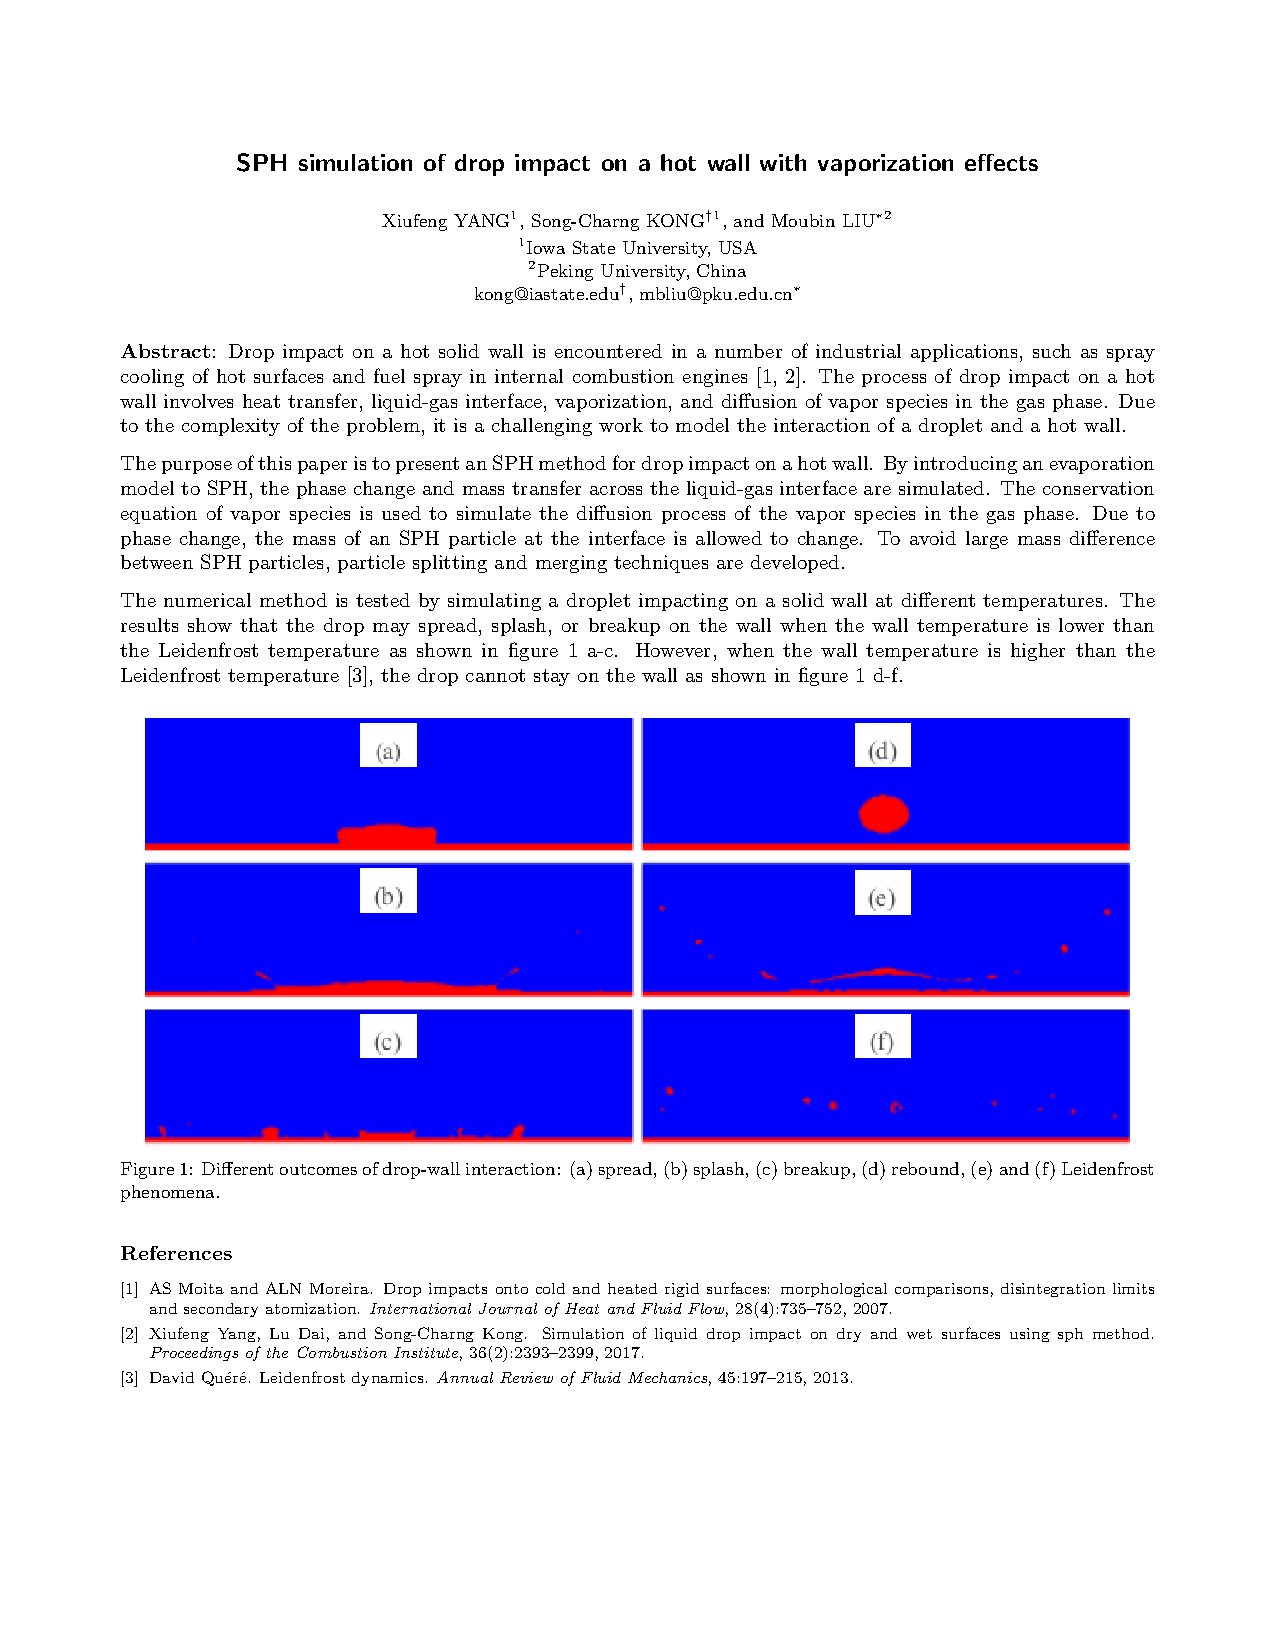
\includepdf[pages=-,pagecommand={\pagestyle{fancy}\label{8.4}},addtotoc={  
     1,subsection,1,SPH simulation of drop impact on a hot wall with vaporization effects,p1}]{abstract/pdfs/9.pdf}



%\section{Session 9: High-Performance Computing}
%9.1: 11
%9.2: 16
%9.3: 26
%9.4: ????????????????????????


\rhead{Session 9}
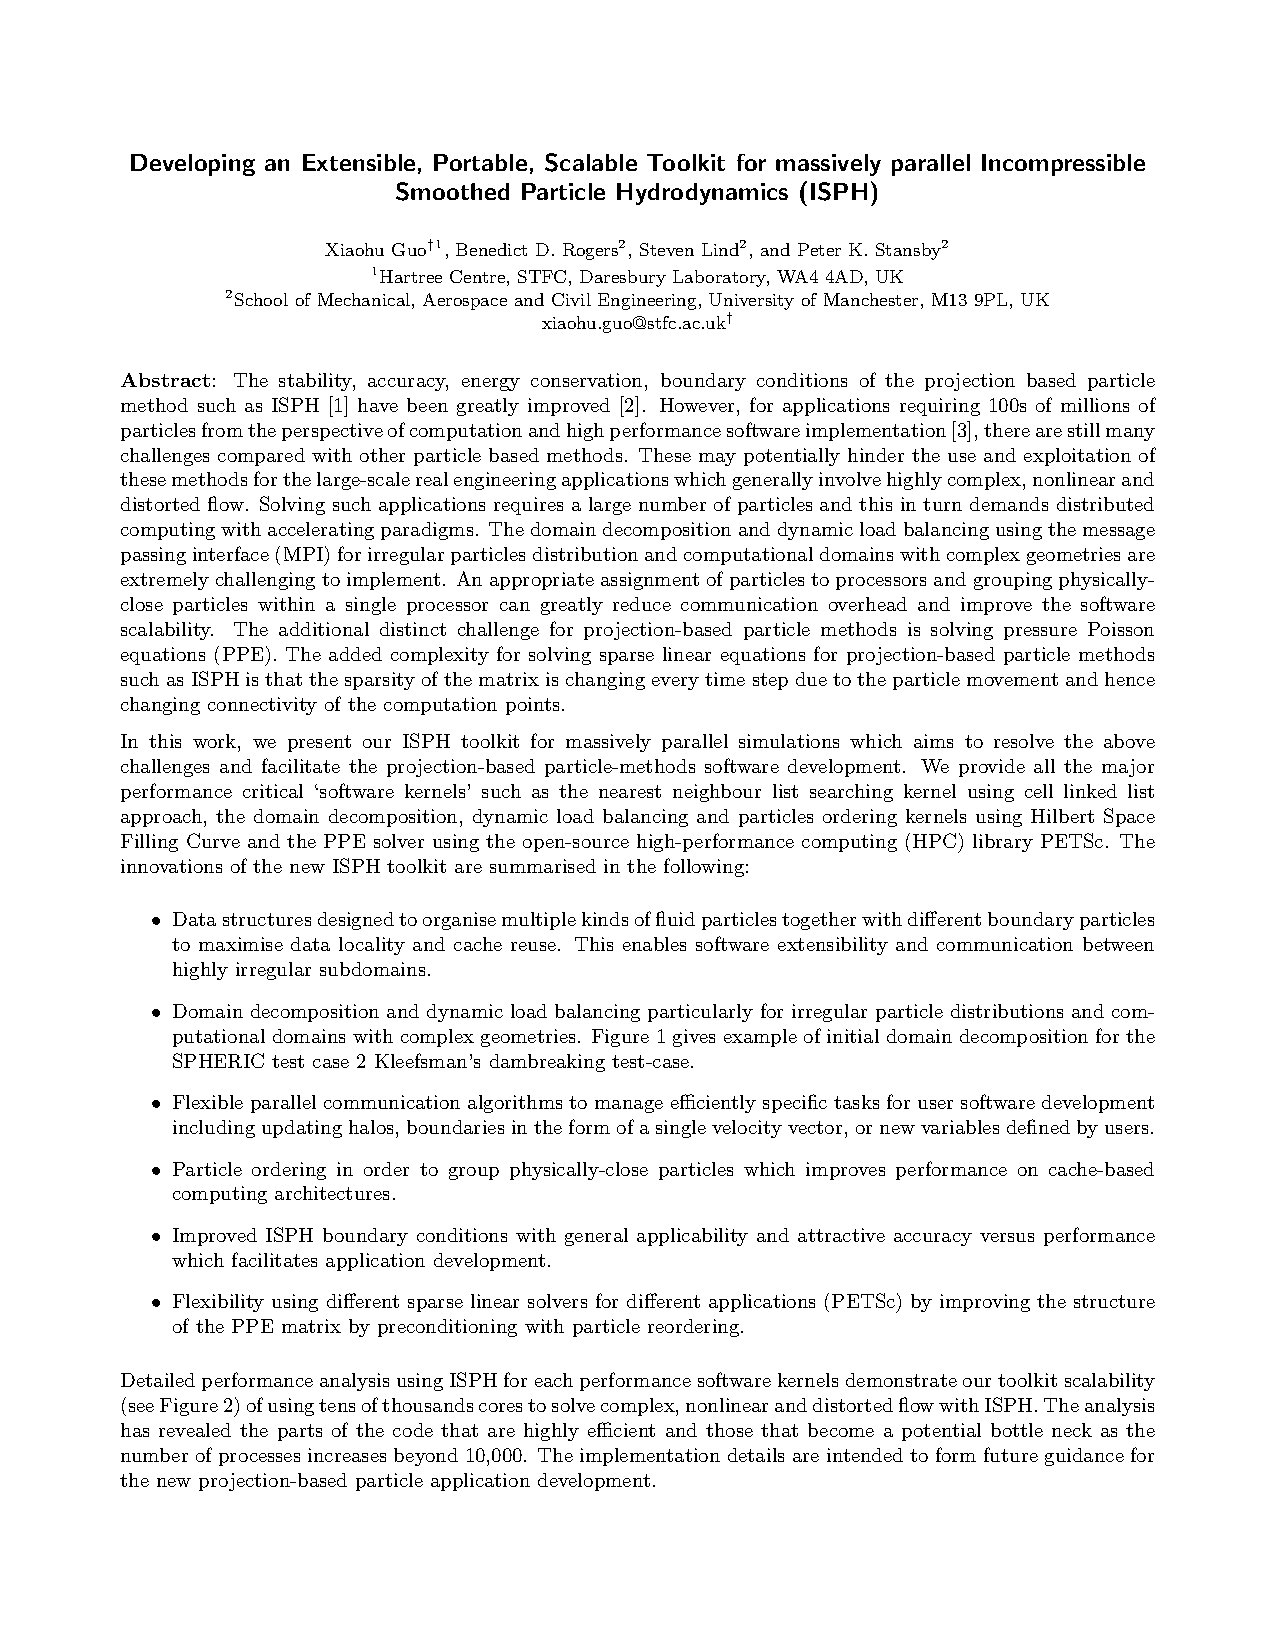
\includepdf[pages=-,pagecommand={\pagestyle{fancy}\label{9.1}},addtotoc={
     1,section,1,{~~~~~~~~High-Performance Computing},p1,   
     1,subsection,1,{Developing an extensible, portable, scalable toolkit for massively parallel incompressible smoothed particle hydrodynamics (ISPH)},p1}]{abstract/pdfs/11.pdf}
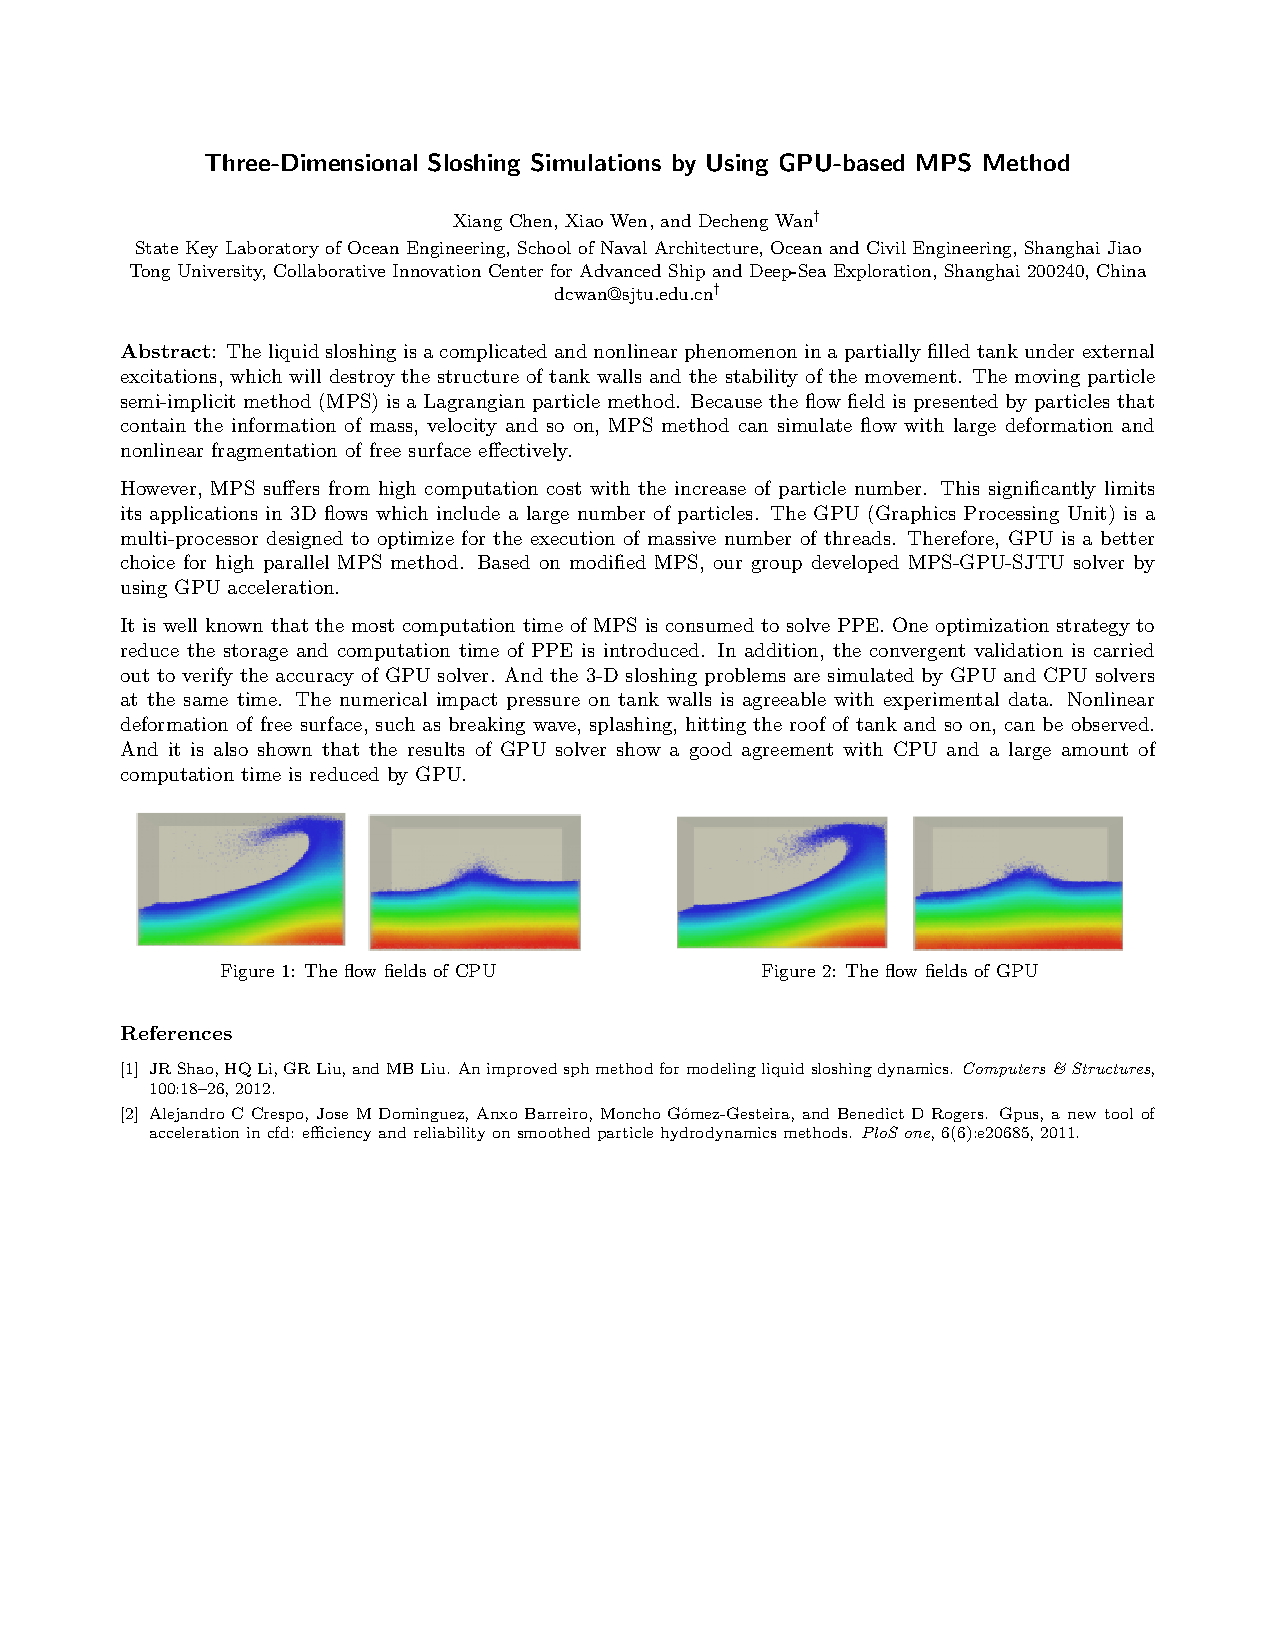
\includepdf[pages=-,pagecommand={\pagestyle{fancy}\label{9.2}},addtotoc={  
     1,subsection,1,Three-dimensional sloshing simulations by using GPU-based MPS method,p1}]{abstract/pdfs/16.pdf}
     
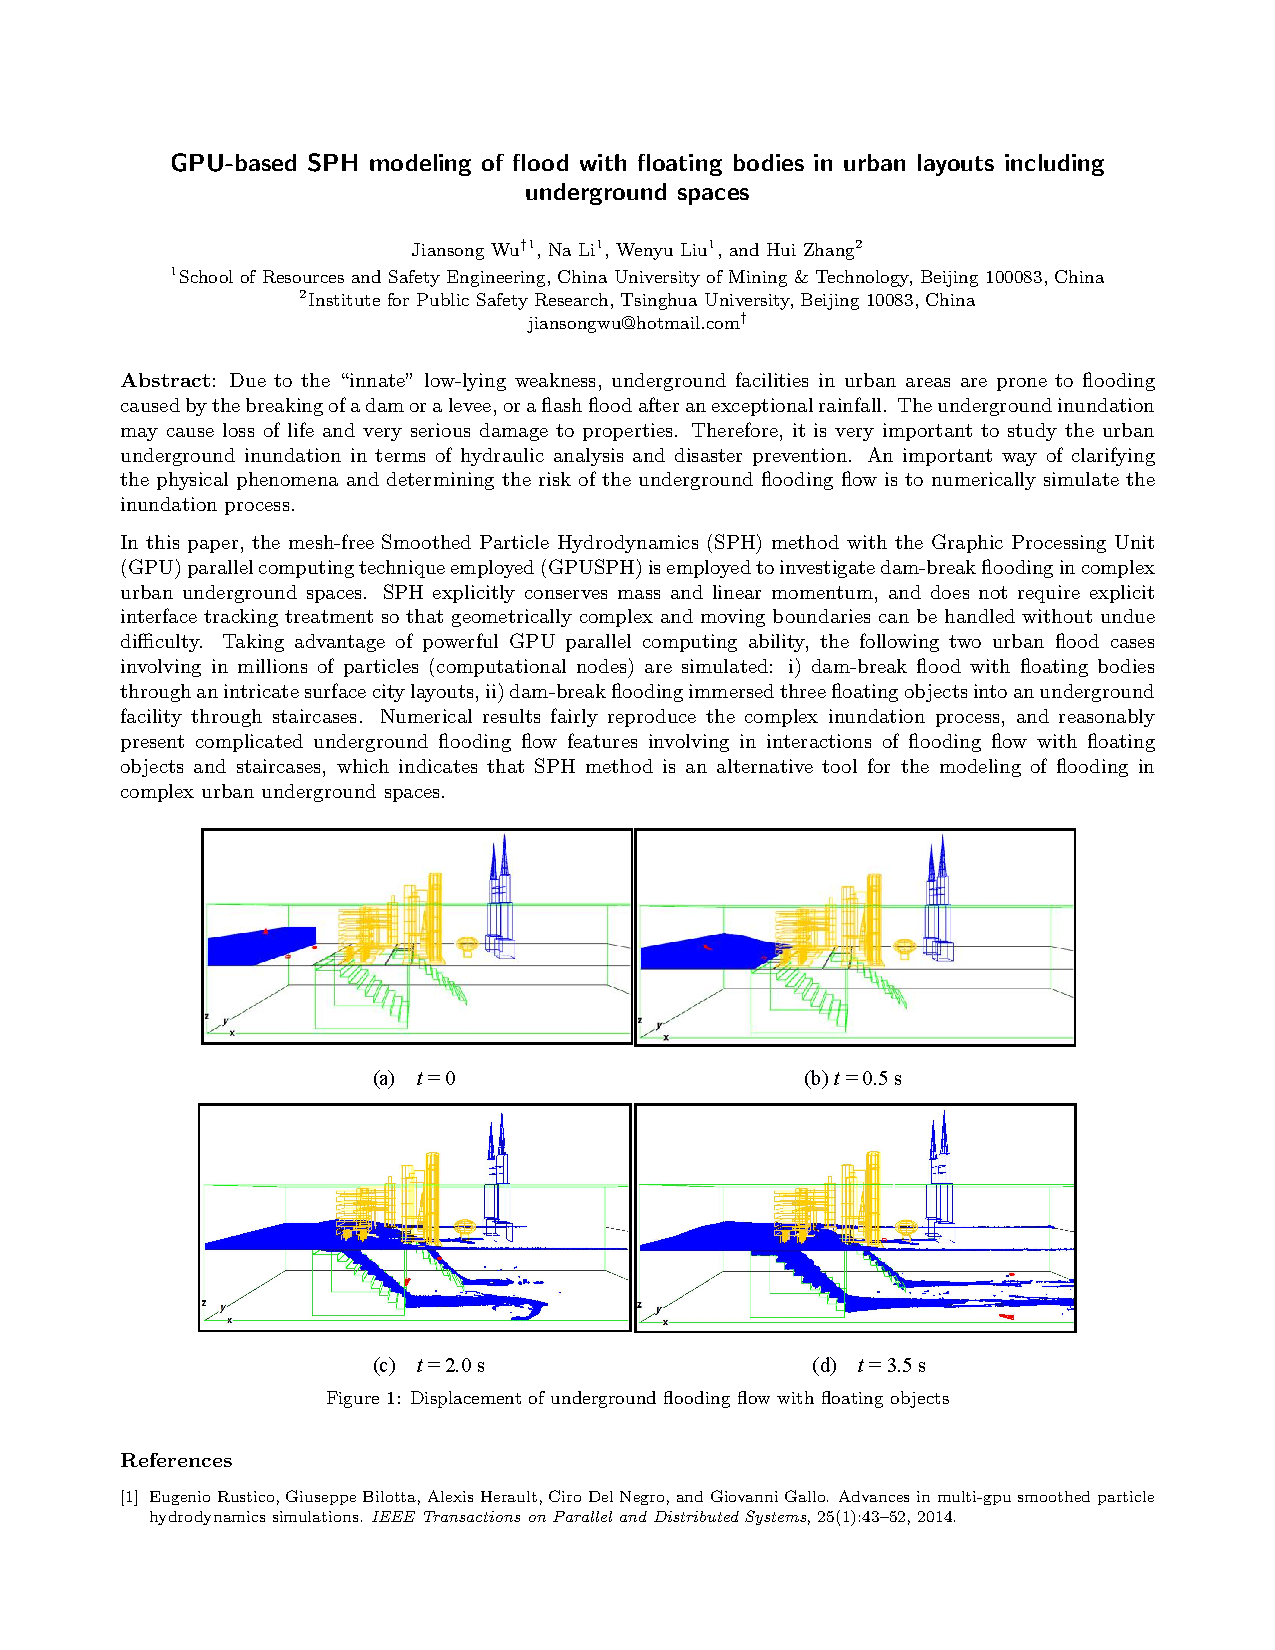
\includepdf[pages=-,pagecommand={\pagestyle{fancy}\label{9.3}},addtotoc={  
     1,subsection,1,GPU-based SPH modeling of flood with floating bodies in urban layouts including underground spaces,p1}]{abstract/pdfs/26.pdf}
%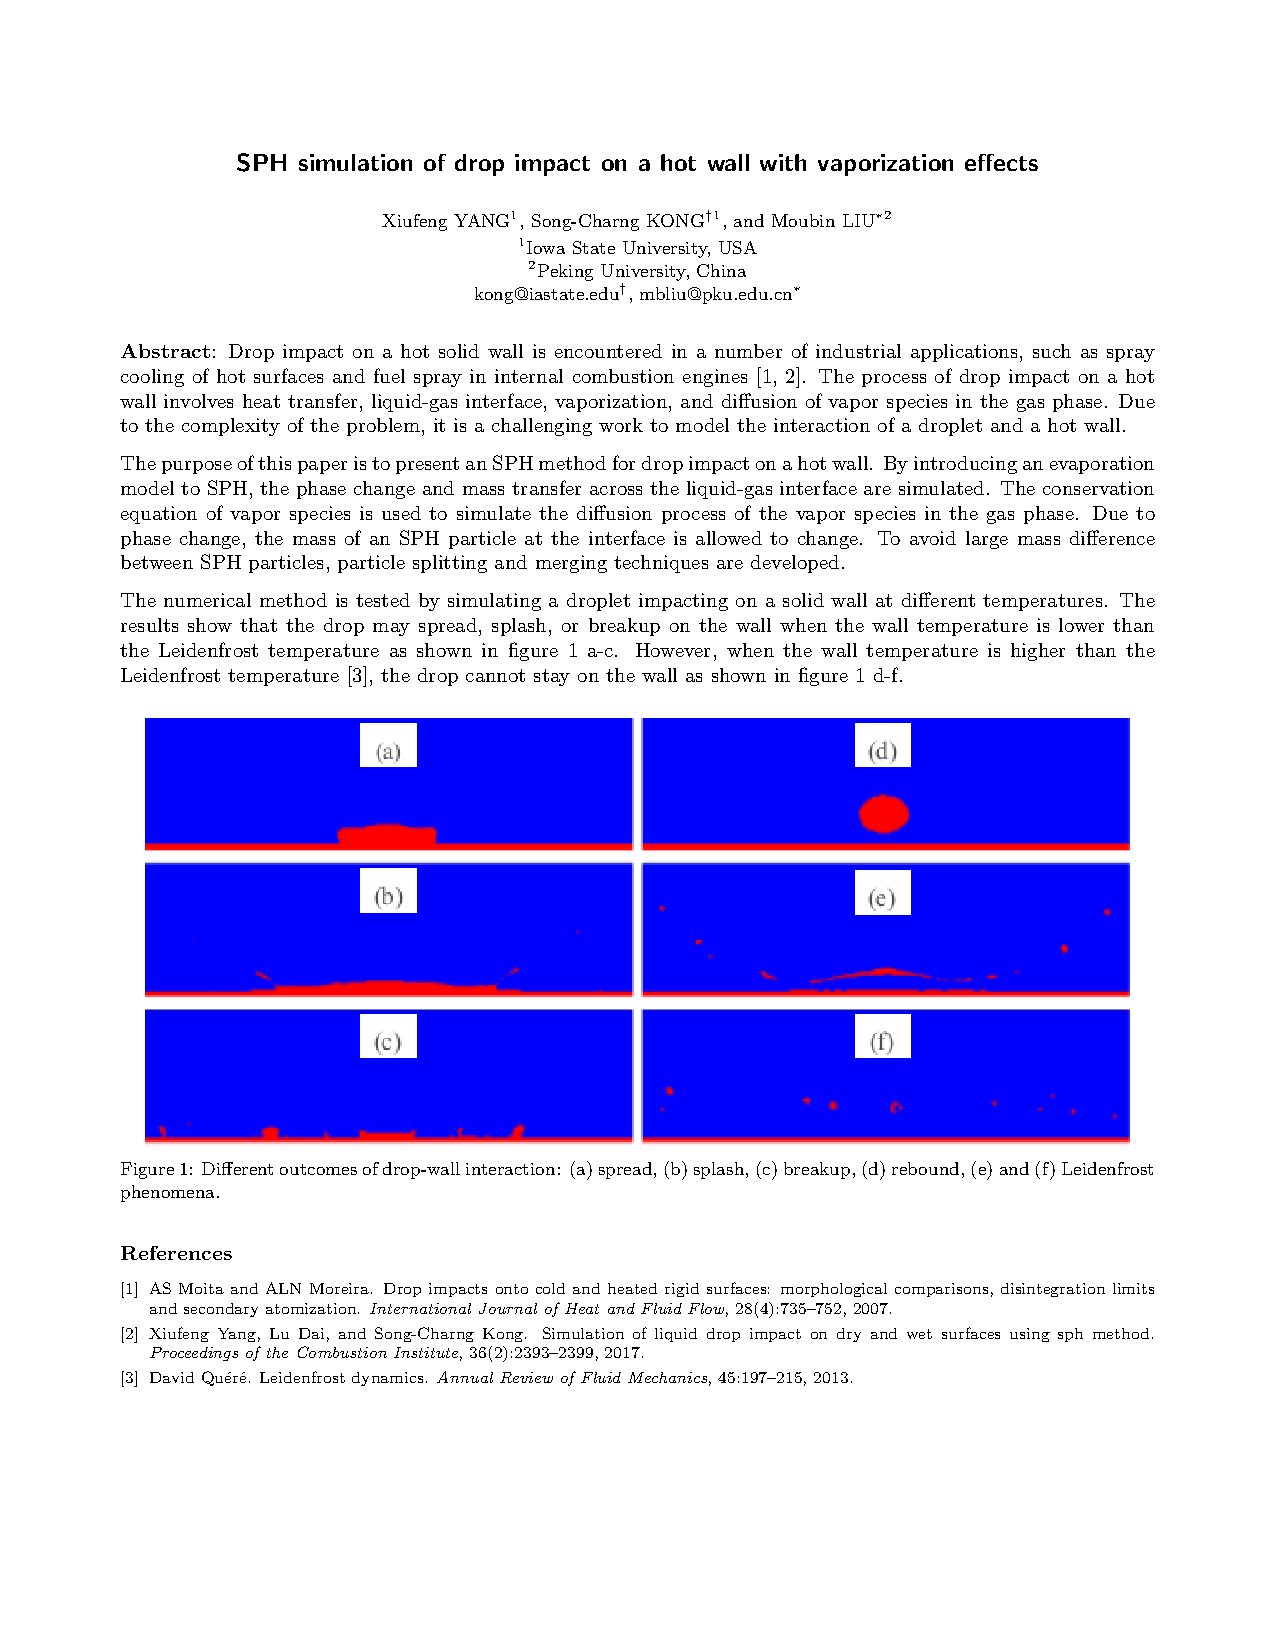
\includepdf[pages=-,pagecommand={\pagestyle{fancy}\label{9.4}},addtotoc={  
%     1,subsection,1,Improve the effectively of computational fluid dynamics work based on supercomputing cloud,p1}]{abstract/pdfs/9.pdf}



%\section{Session 10: Numerical Aspects of SPH}
%10.1: 43
%10.2: 49
%10.3: 52
%10.4: 50

\rhead{Session 10}
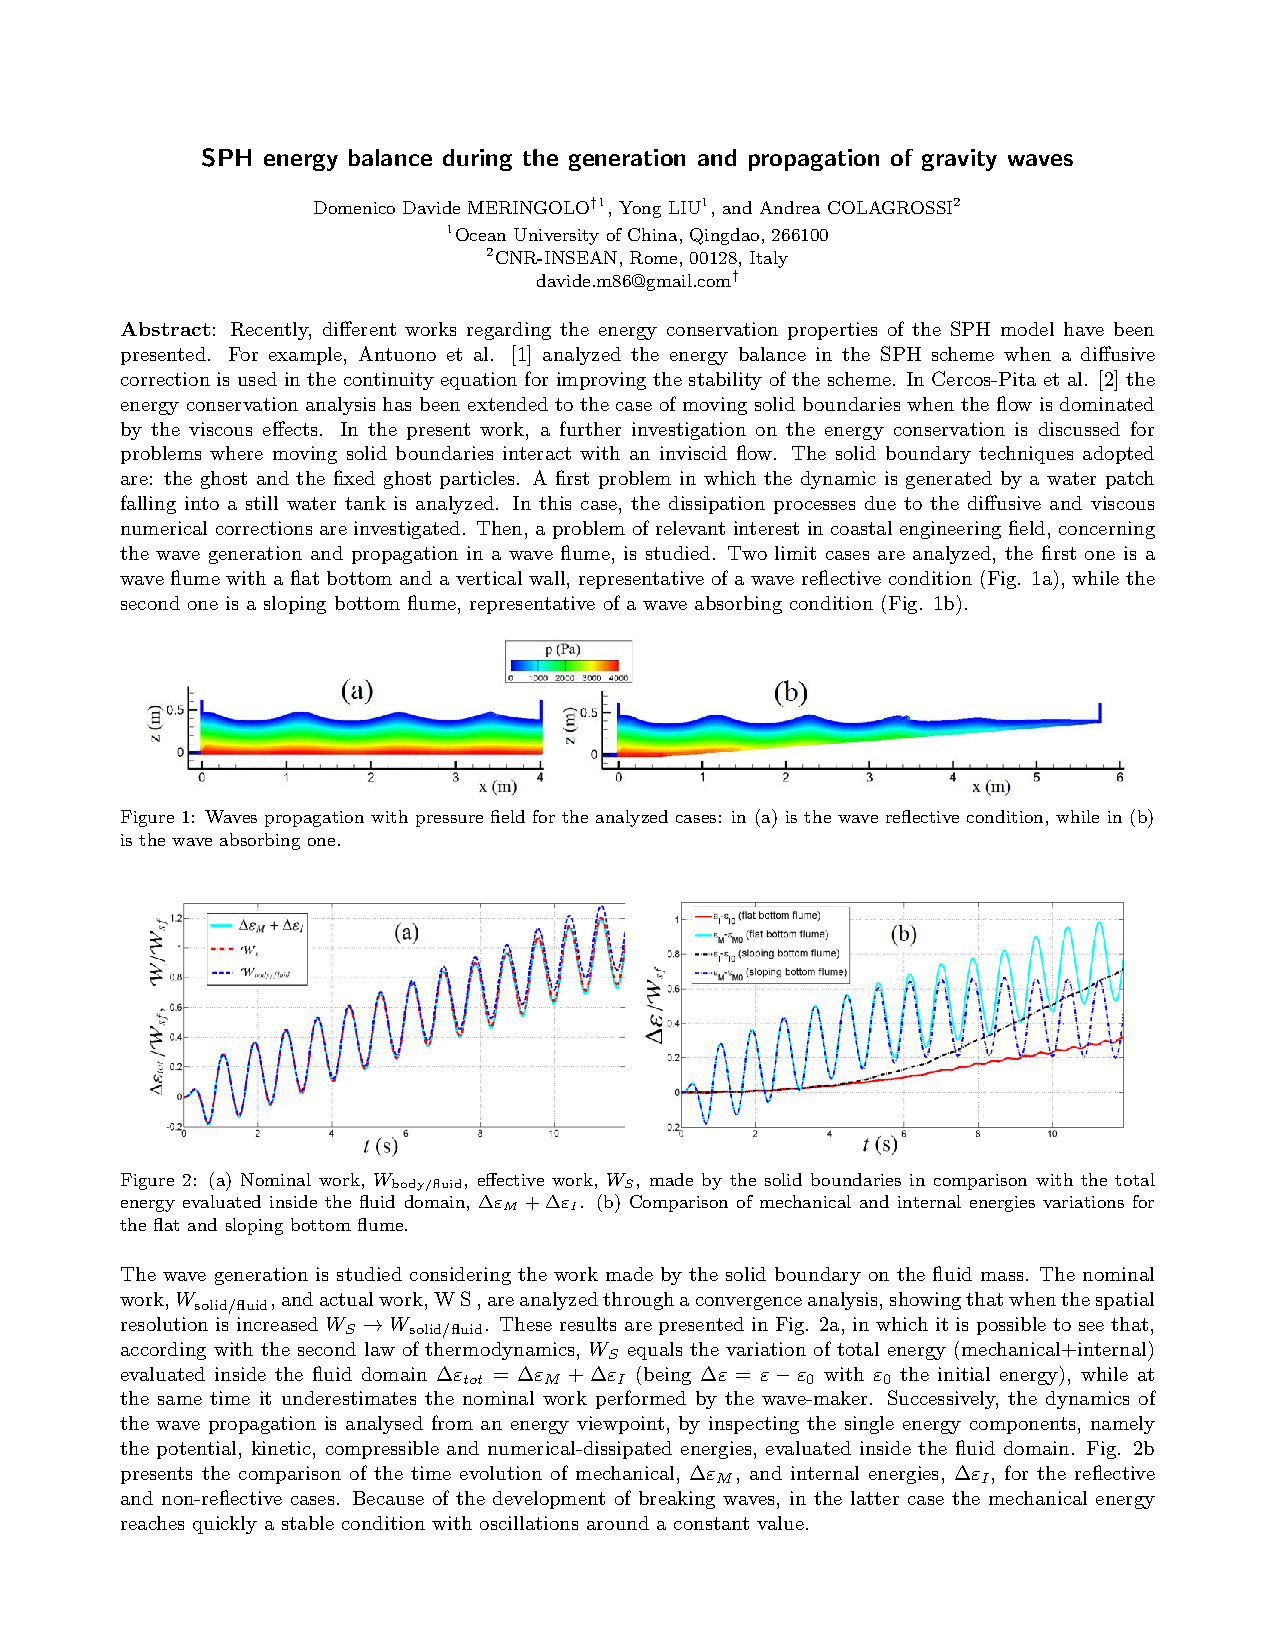
\includepdf[pages=-,pagecommand={\pagestyle{fancy}\label{10.1}},addtotoc={
     1,section,1,{~~~~~~~~Numerical Aspects of SPH},p1,   
     1,subsection,1,SPH energy balance during the generation and propagation of gravity waves,p1}]{abstract/pdfs/43.pdf}
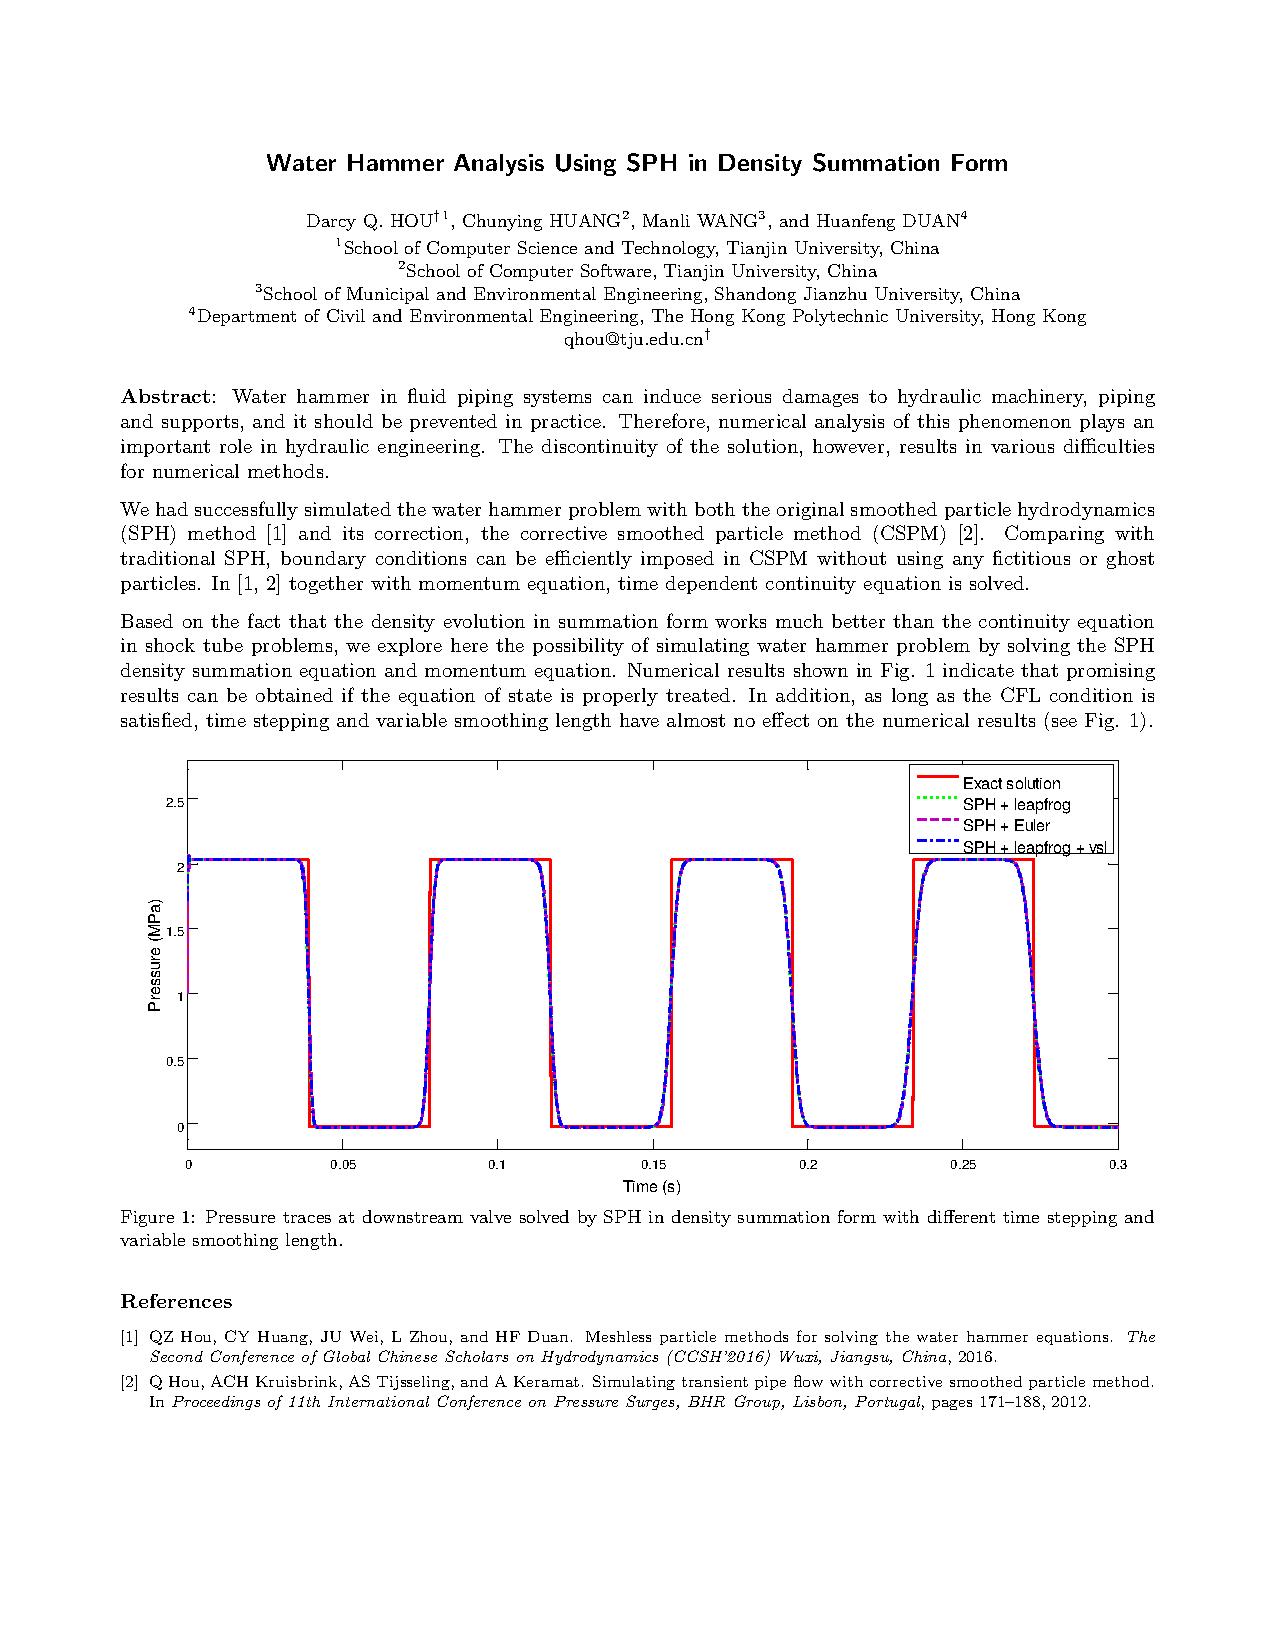
\includepdf[pages=-,pagecommand={\pagestyle{fancy}\label{10.2}},addtotoc={  
     1,subsection,1,Water hammer analysis using SPH in density summation form,p1}]{abstract/pdfs/49.pdf}
\includepdf[pages=-,pagecommand={\pagestyle{fancy}\label{10.3}},addtotoc={  
     1,subsection,1,Particle trajectory calculation in SPH,p1}]{abstract/pdfs/52.pdf}
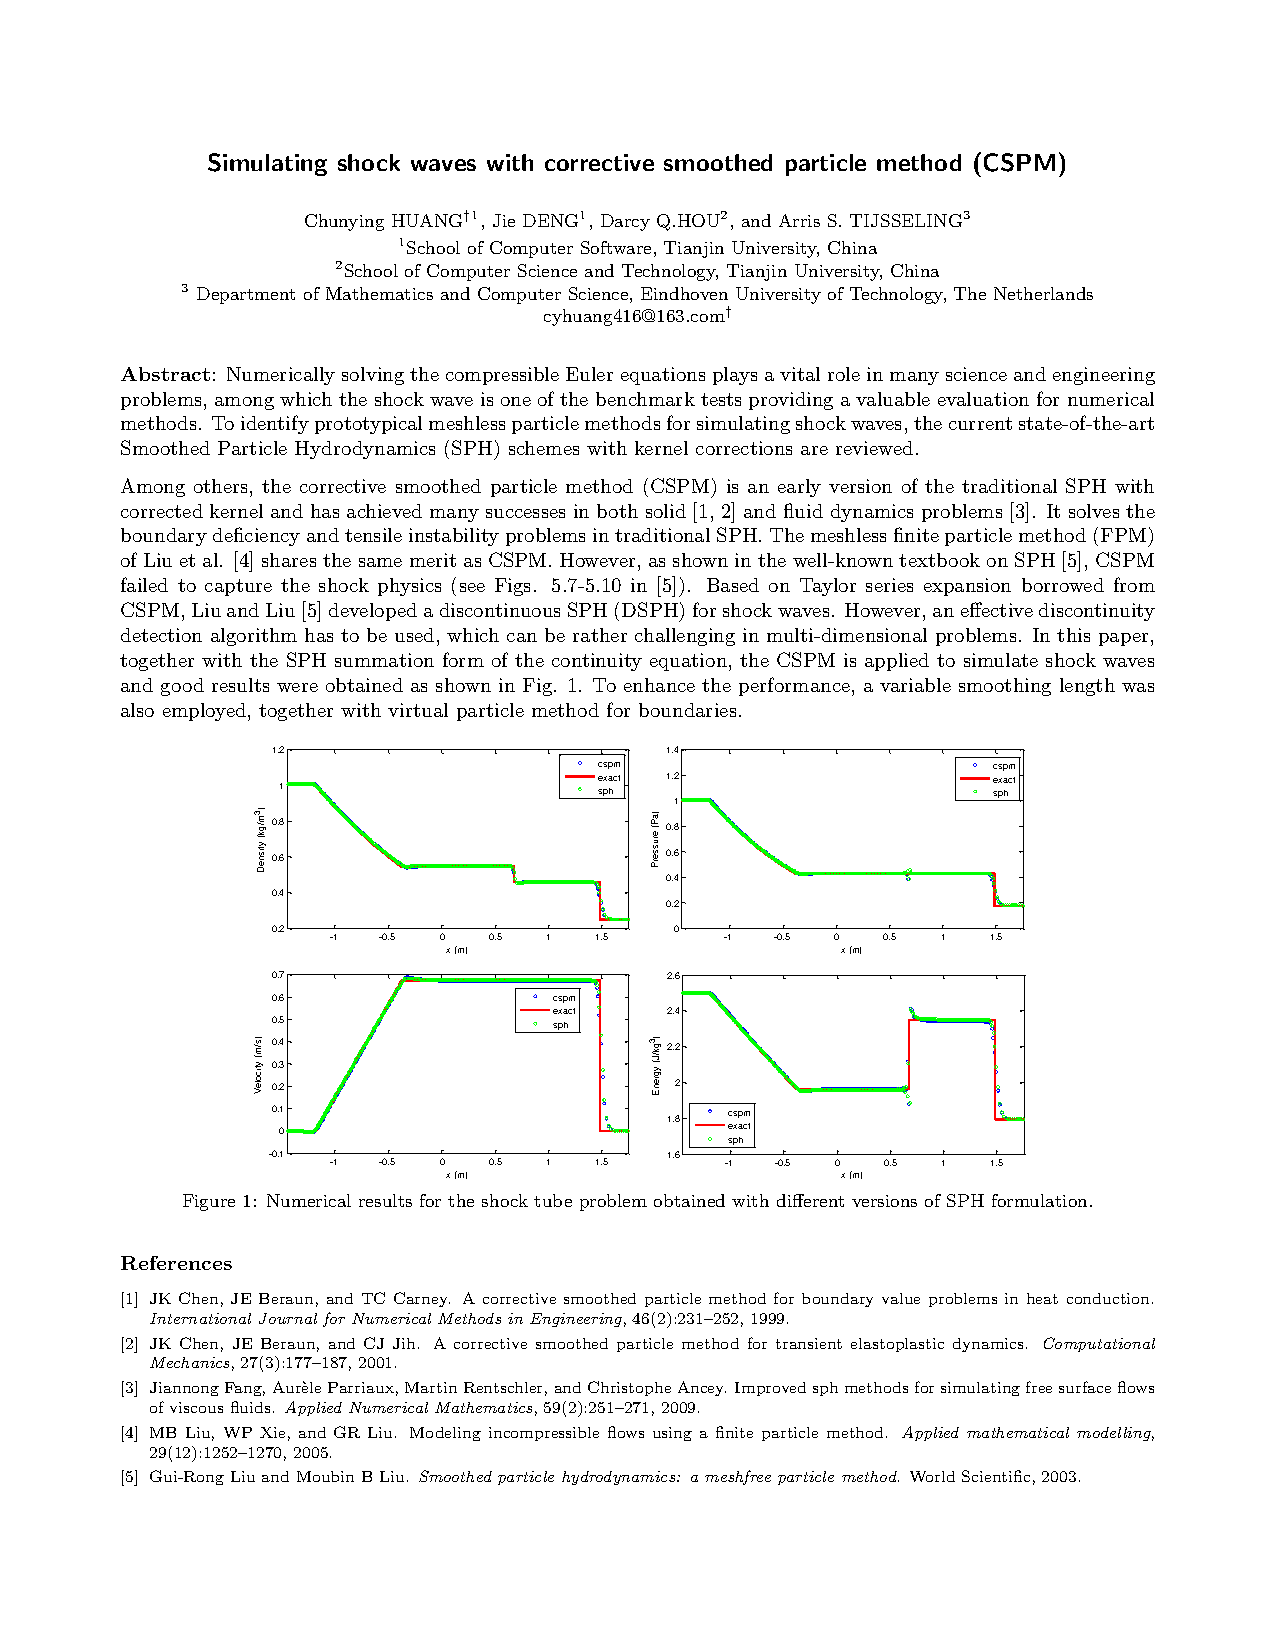
\includepdf[pages=-,pagecommand={\pagestyle{fancy}\label{10.4}},addtotoc={  
     1,subsection,1,Simulating shock waves with corrective smoothed particle method (CSPM),p1}]{abstract/pdfs/50.pdf}



%\section{Session 11: Fluid Structure Interaction}
%11.1: 7 
%11.2: 42
%11.3: 19
%11.4: 45


\rhead{Session 11}
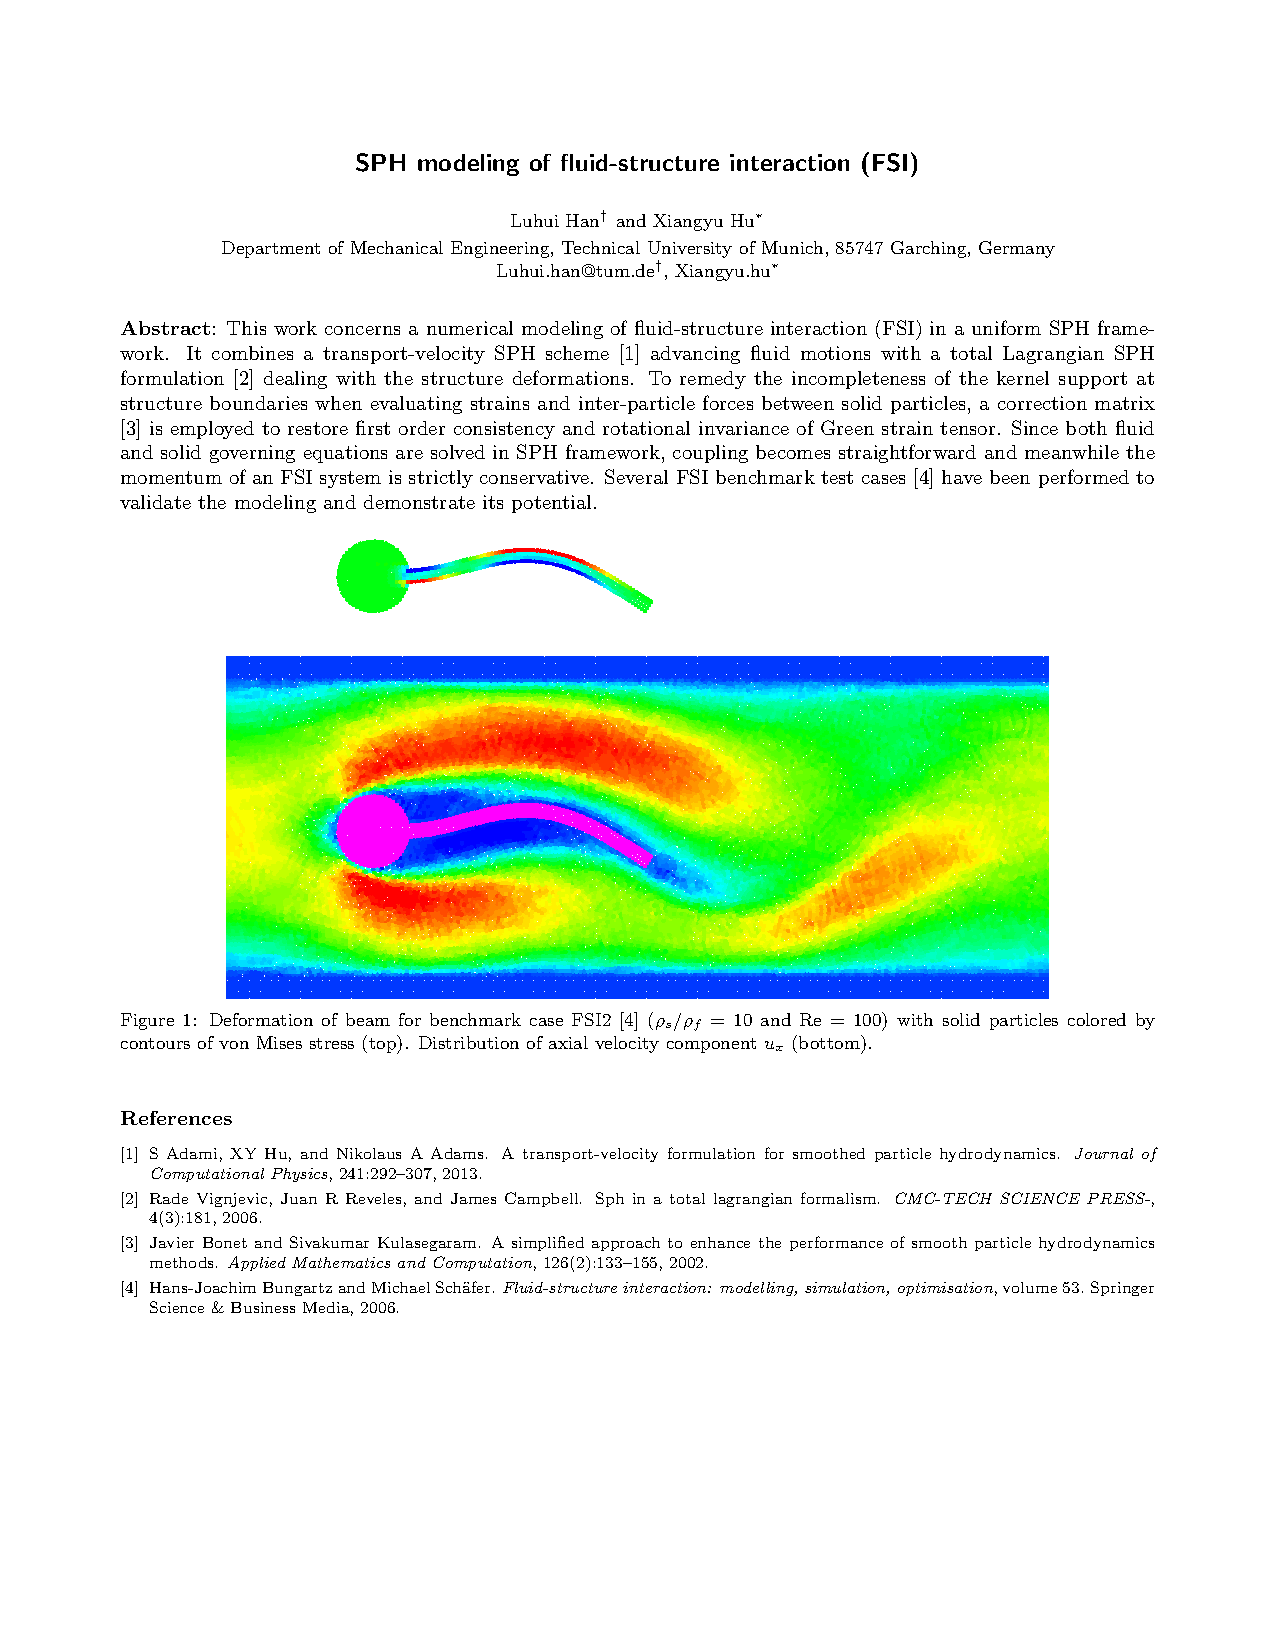
\includepdf[pages=-,pagecommand={\pagestyle{fancy}\label{11.1}},addtotoc={
     1,section,1,{~~~~~~~~Fluid Structure Interaction},p1,   
     1,subsection,1,SPH modeling of fluid-structure interaction (FSI),p1}]{abstract/pdfs/7.pdf}
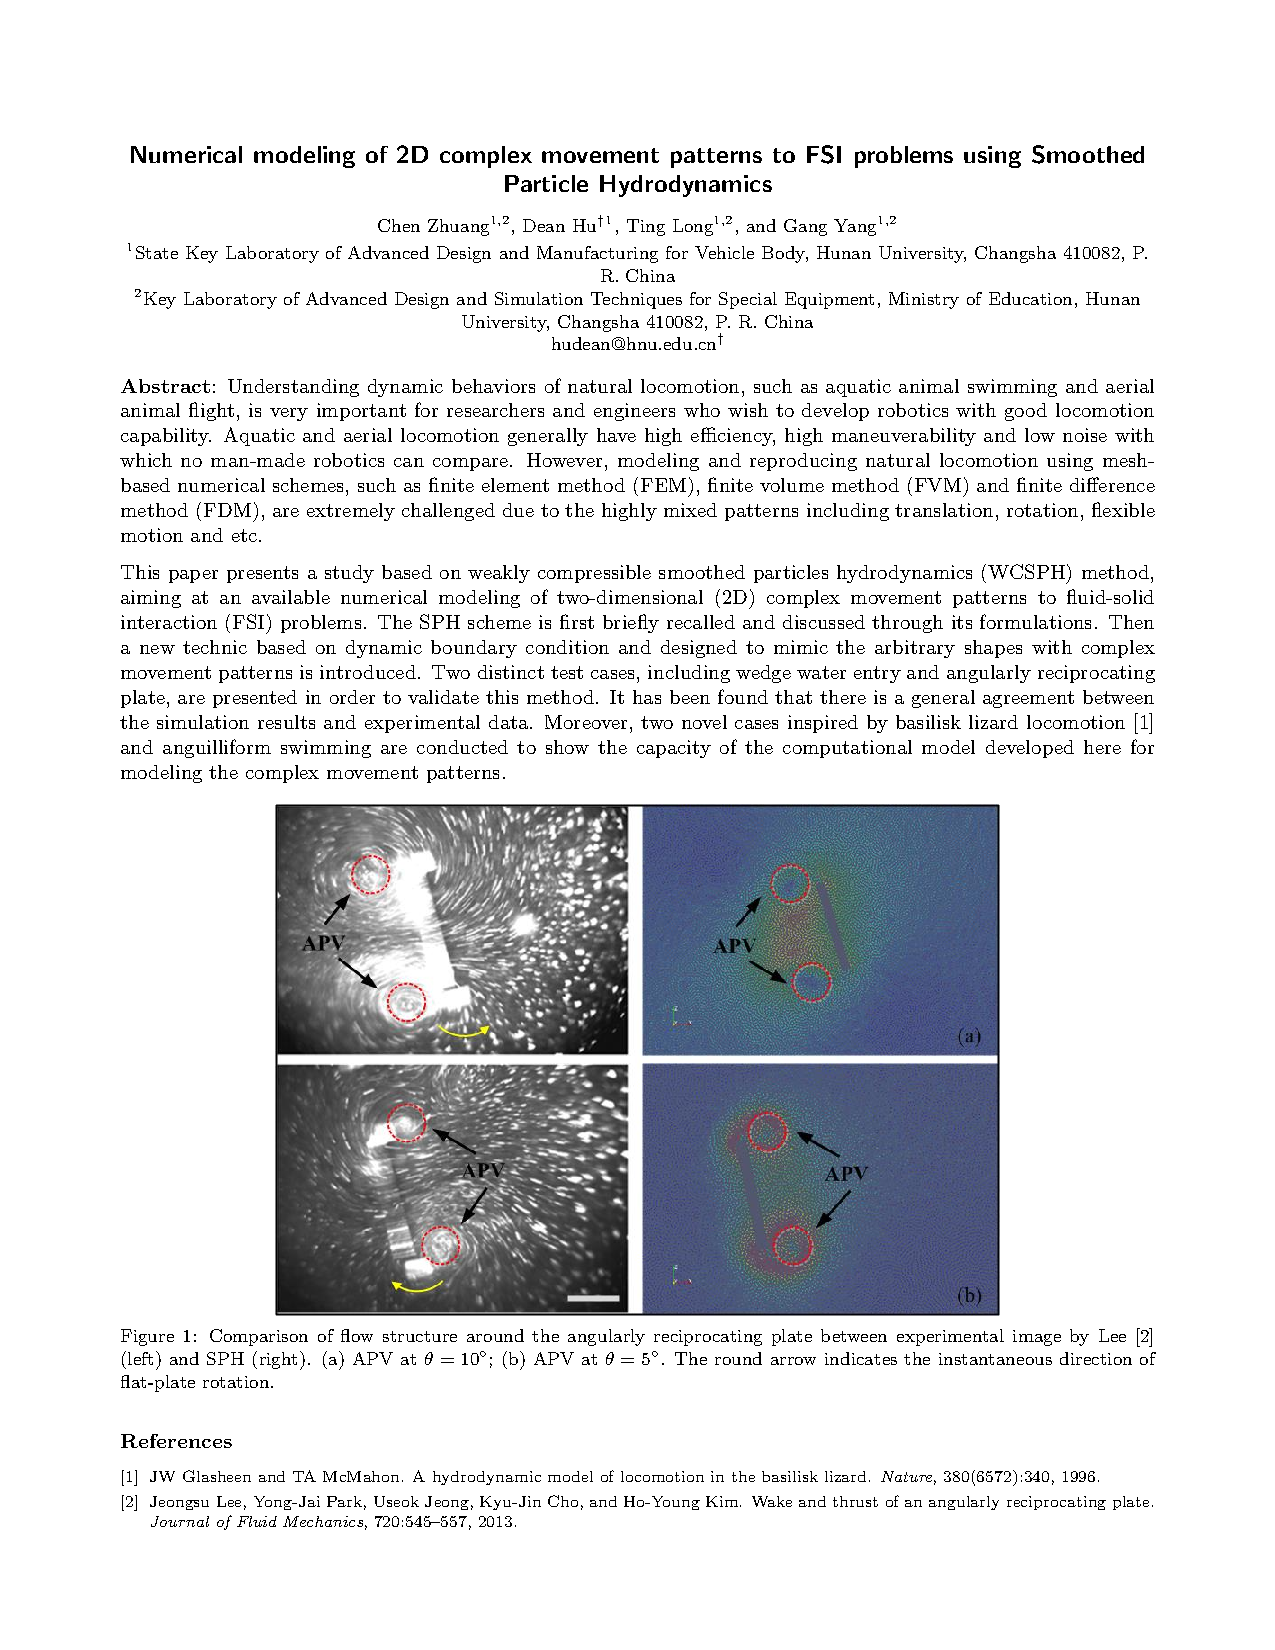
\includepdf[pages=-,pagecommand={\pagestyle{fancy}\label{11.2}},addtotoc={  
     1,subsection,1,Numerical modeling of 2D complex movement patterns to FSI problems using smoothed particle hydrodynamics,p1}]{abstract/pdfs/42.pdf}
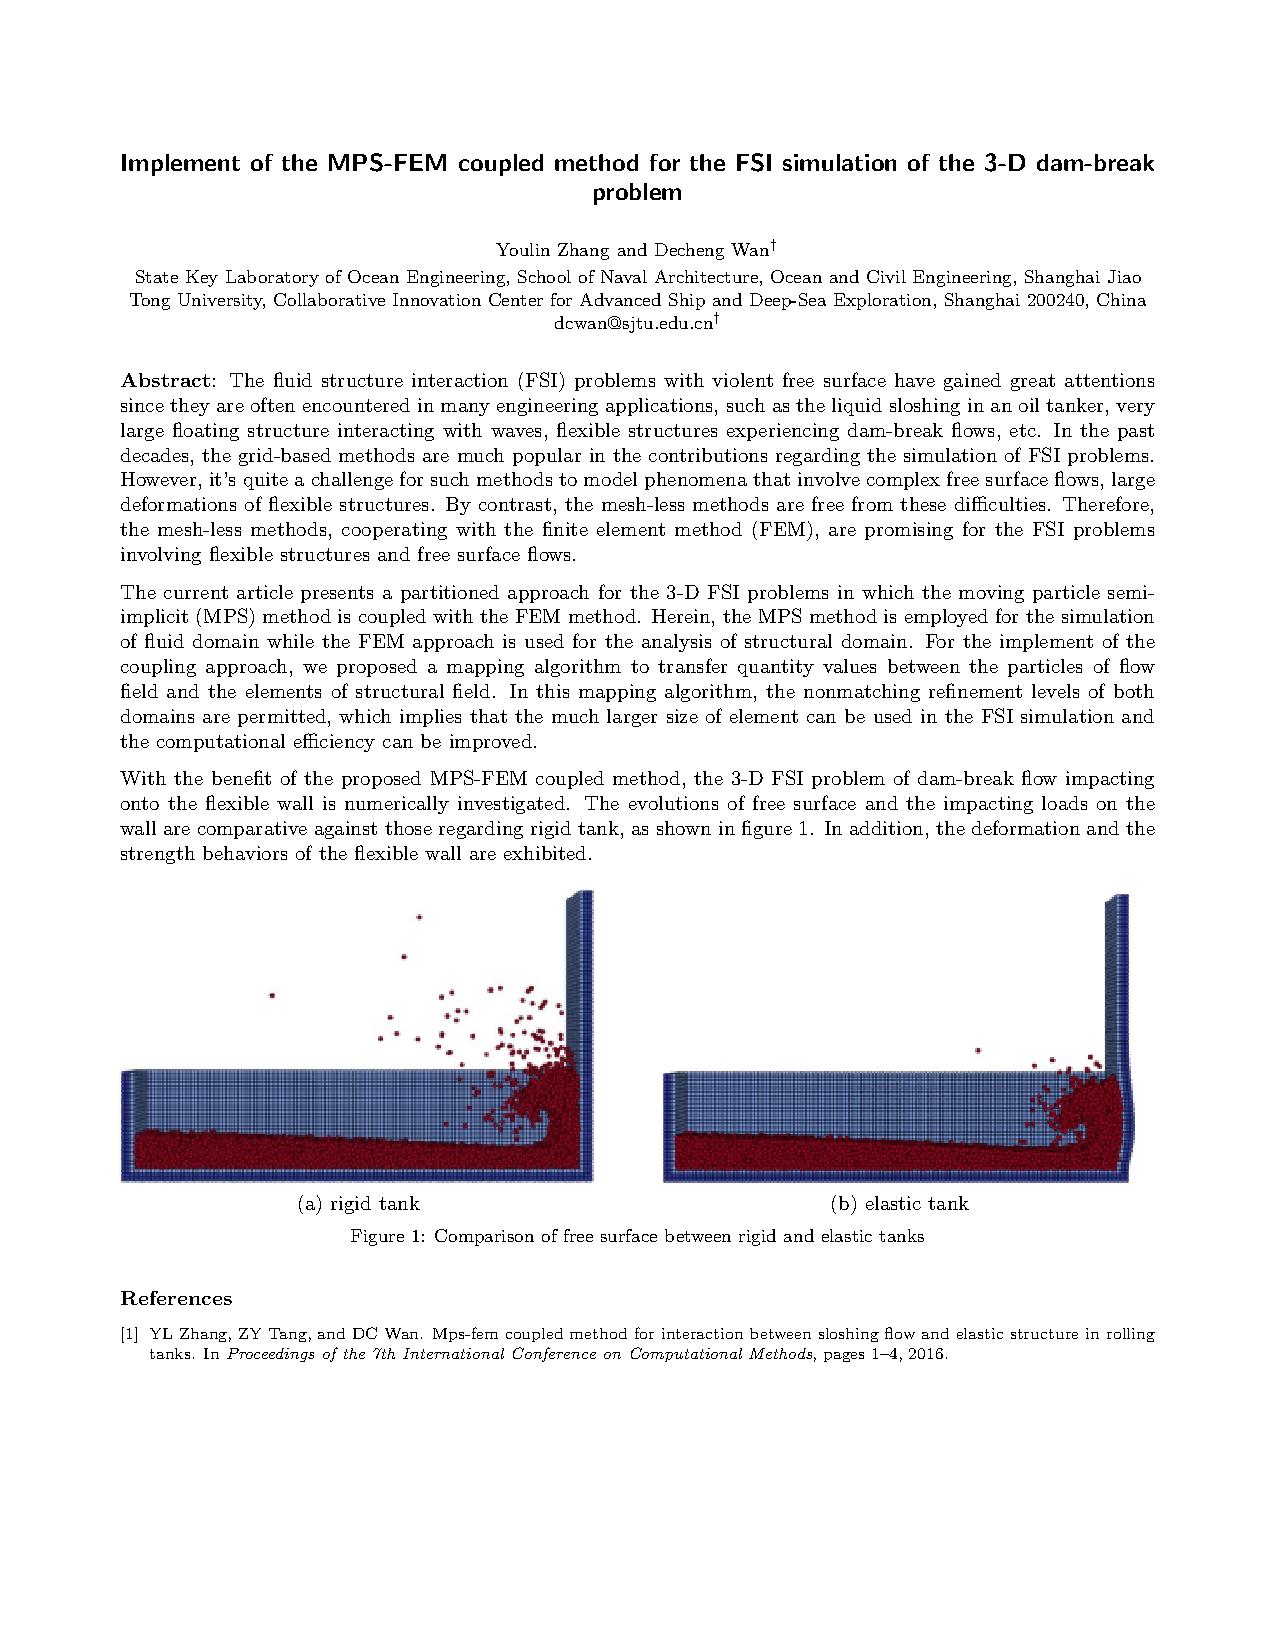
\includepdf[pages=-,pagecommand={\pagestyle{fancy}\label{11.3}},addtotoc={  
     1,subsection,1,Implement of the MPS-FEM coupled method for the FSI simulation of the 3-D dam-break problem,p1}]{abstract/pdfs/19.pdf}
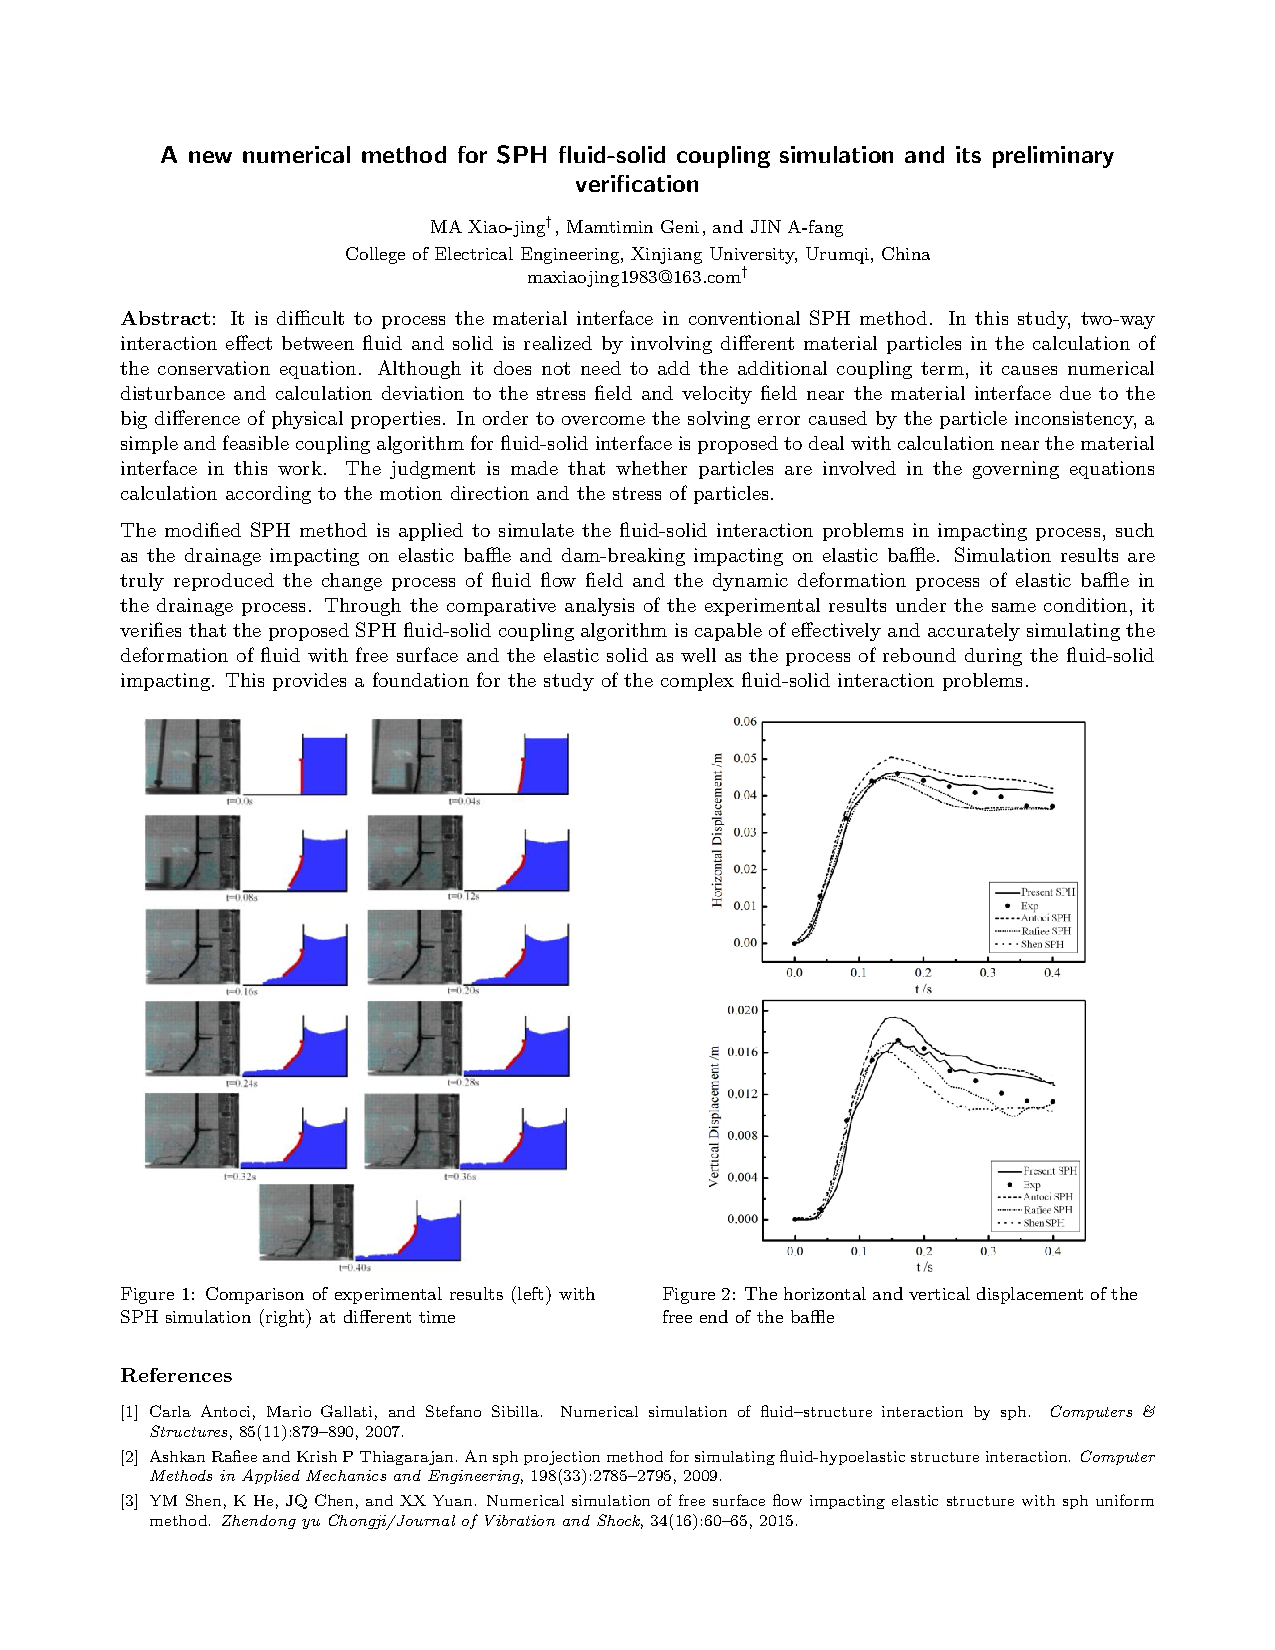
\includepdf[pages=-,pagecommand={\pagestyle{fancy}\label{11.4}},addtotoc={  
     1,subsection,1,A new numerical method for SPH fluid-solid coupling simulation and its preliminary verification,p1}]{abstract/pdfs/45.pdf}


%\section{Session 12: Modelling of Incompressible Flows}
%12.1: 2
%12.2: 17
%12.3: 27    
%12.4: 18

\rhead{Session 12}
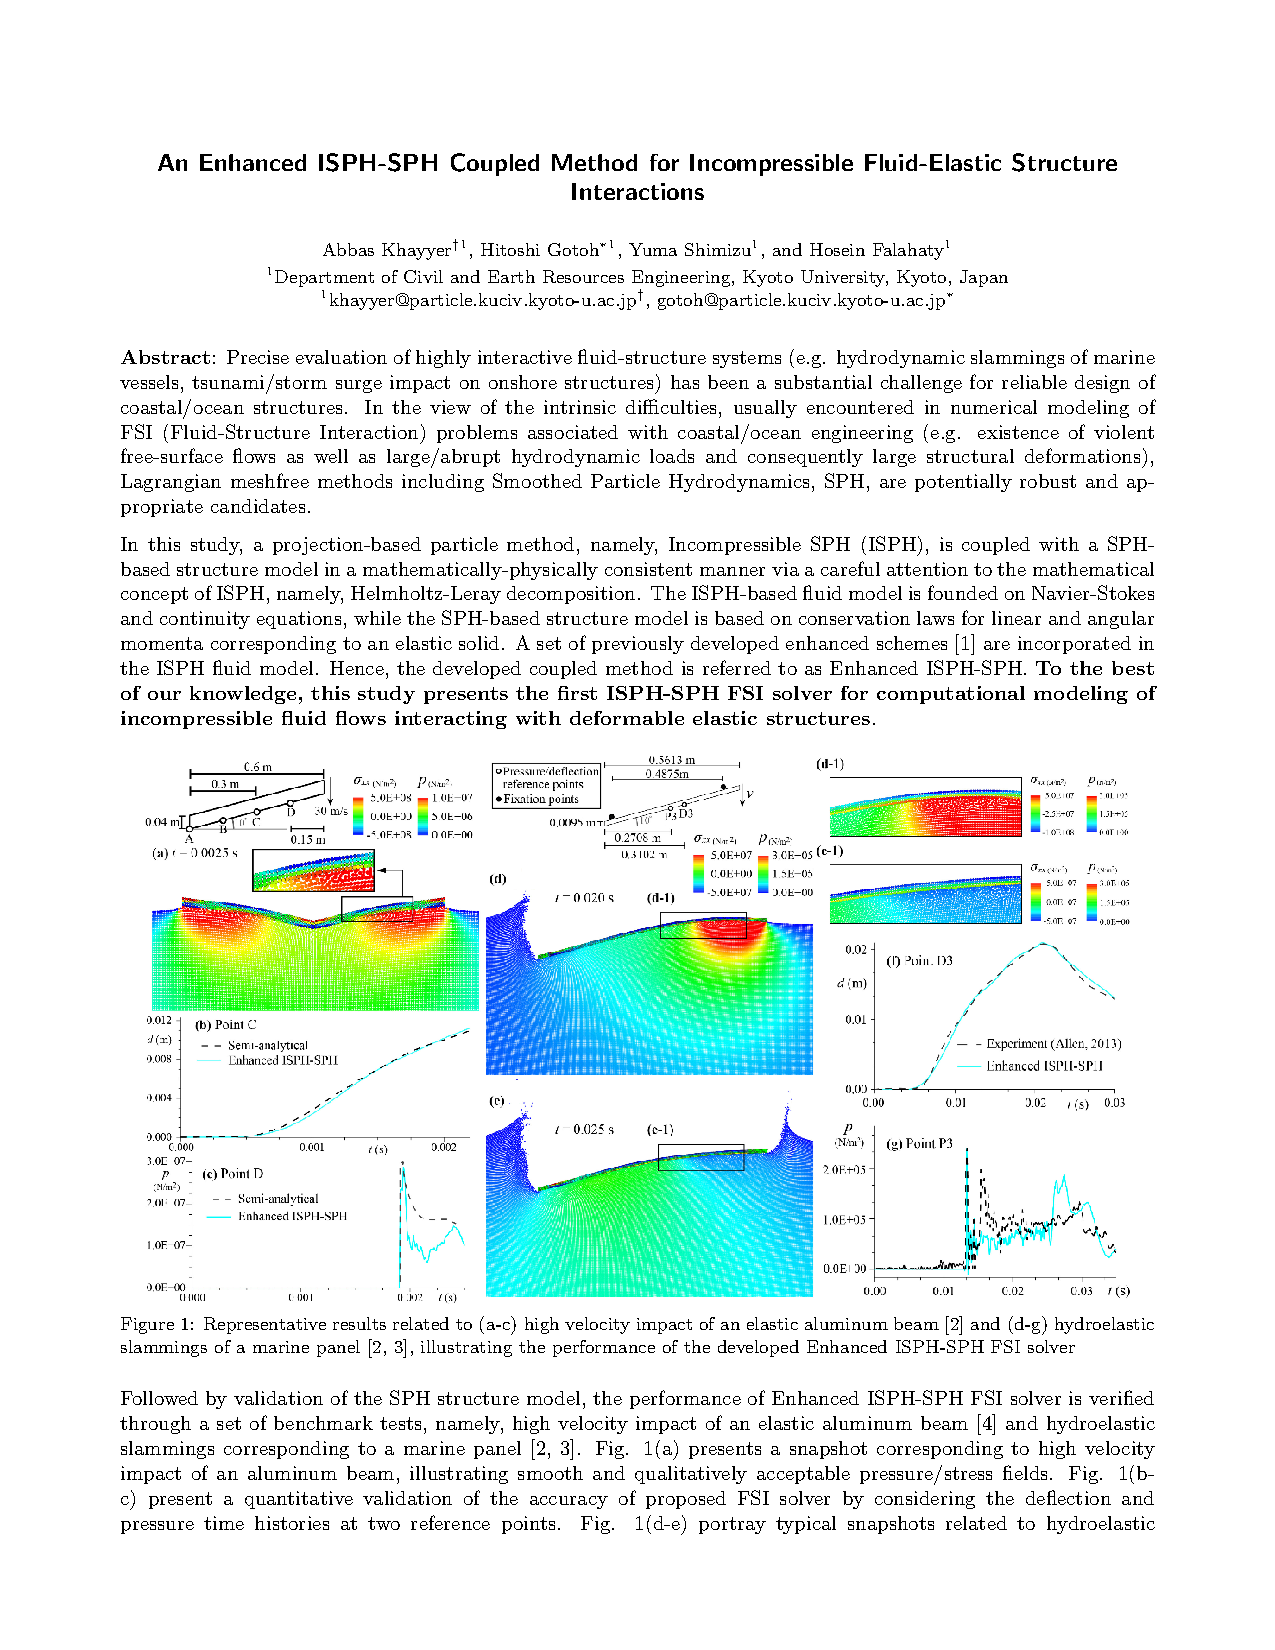
\includepdf[pages=-,pagecommand={\pagestyle{fancy}\label{12.1}},addtotoc={
     1,section,1,{~~~~~~~~Modelling of Incompressible Flows},p1,   
     1,subsection,1,An enhanced ISPH-SPH coupled method for incompressible fluid-elastic structure interactions,p1}]{abstract/pdfs/2.pdf}
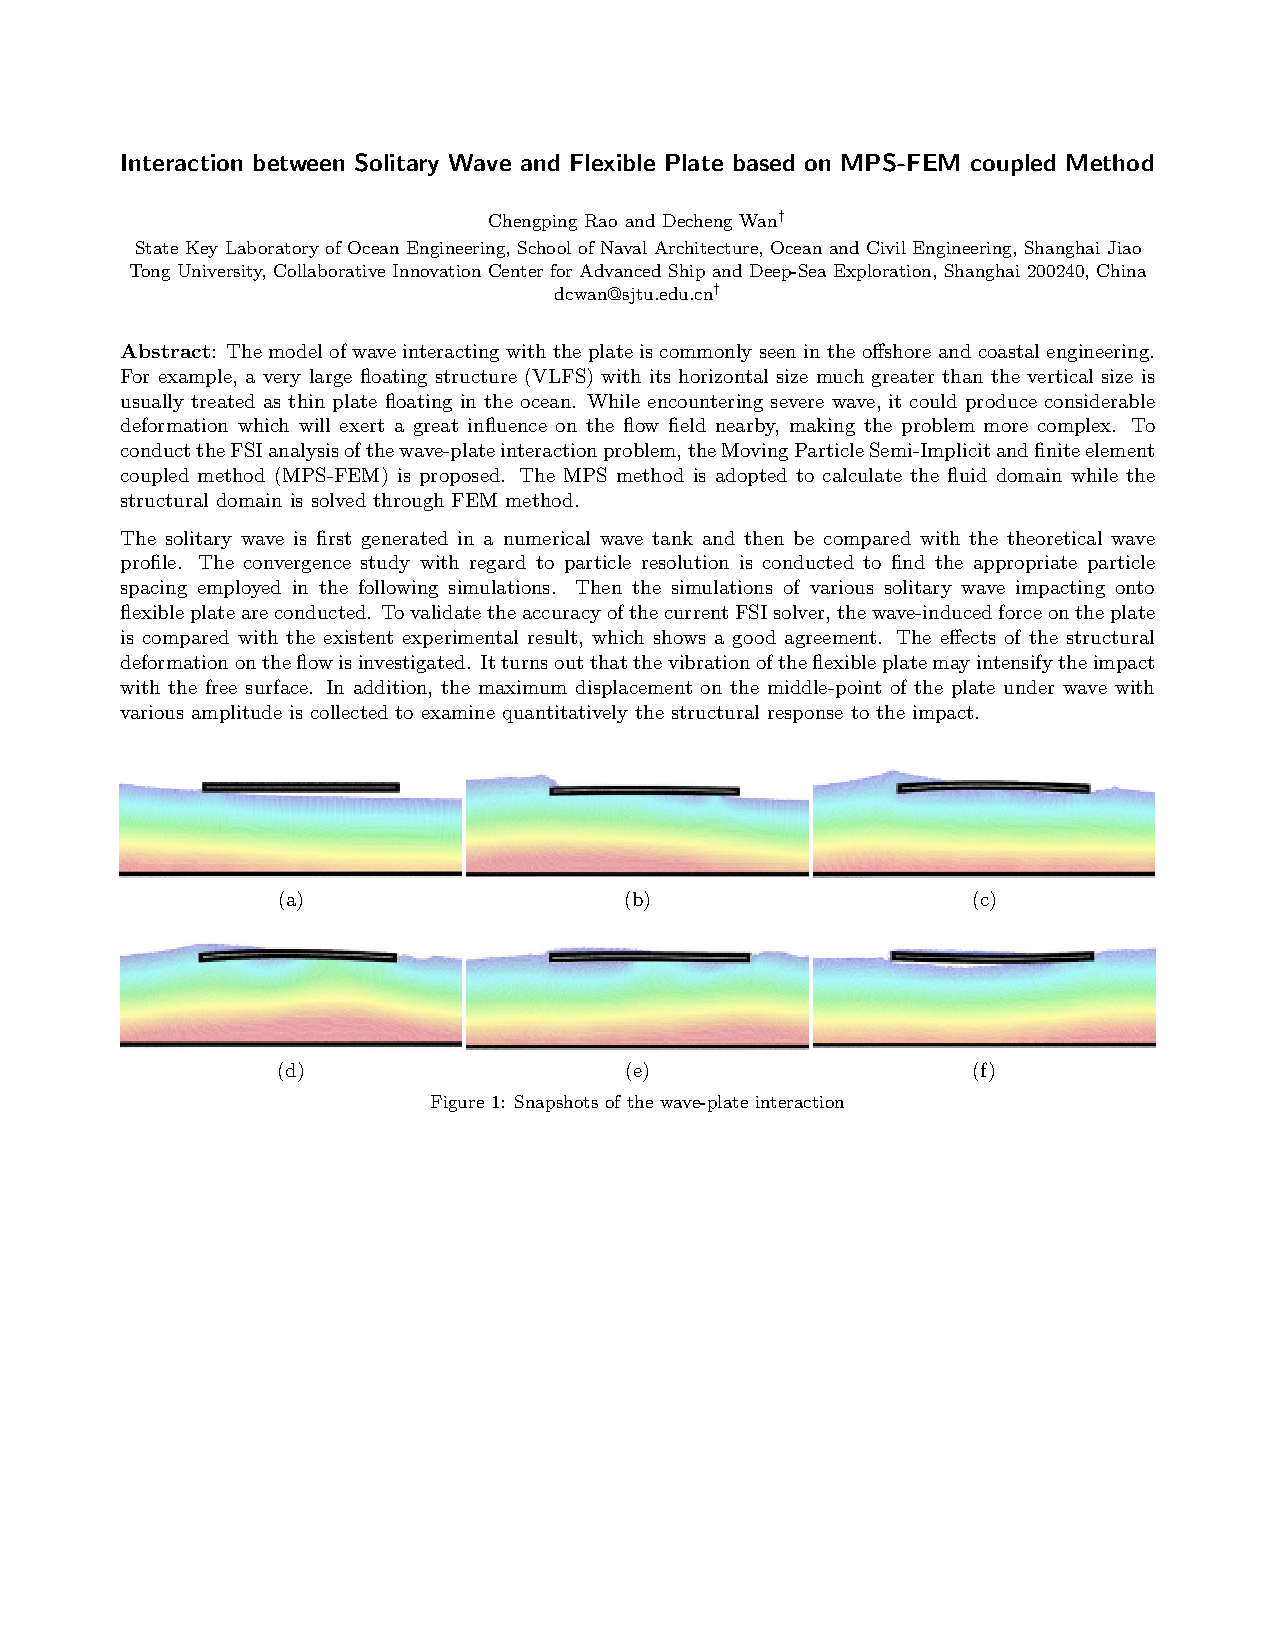
\includepdf[pages=-,pagecommand={\pagestyle{fancy}\label{12.2}},addtotoc={  
     1,subsection,1,Interaction between solitary wave and flexible plate based on MPS-FEM coupled method,p1}]{abstract/pdfs/17.pdf}
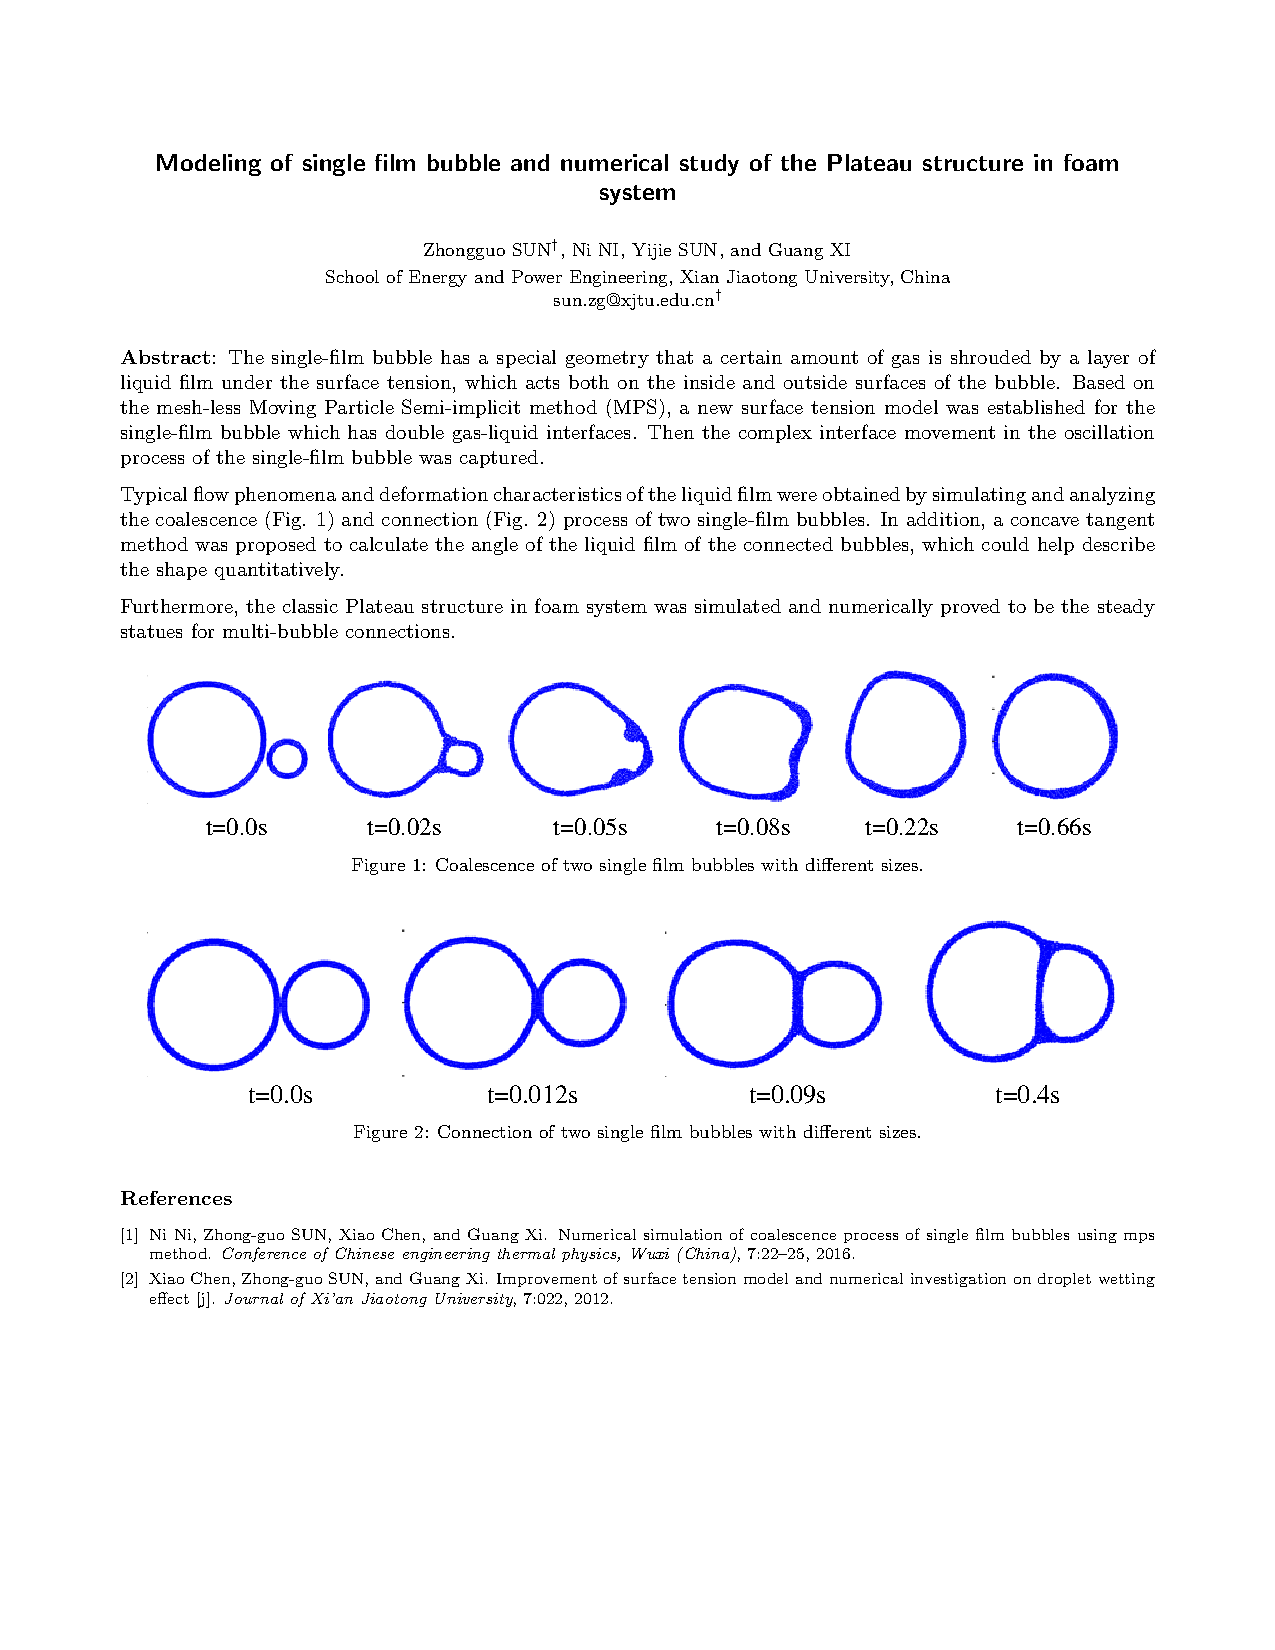
\includepdf[pages=-,pagecommand={\pagestyle{fancy}\label{12.3}},addtotoc={  
     1,subsection,1,Modeling of single film bubble and numerical study of the plateau structure in foam system,p1}]{abstract/pdfs/27.pdf}
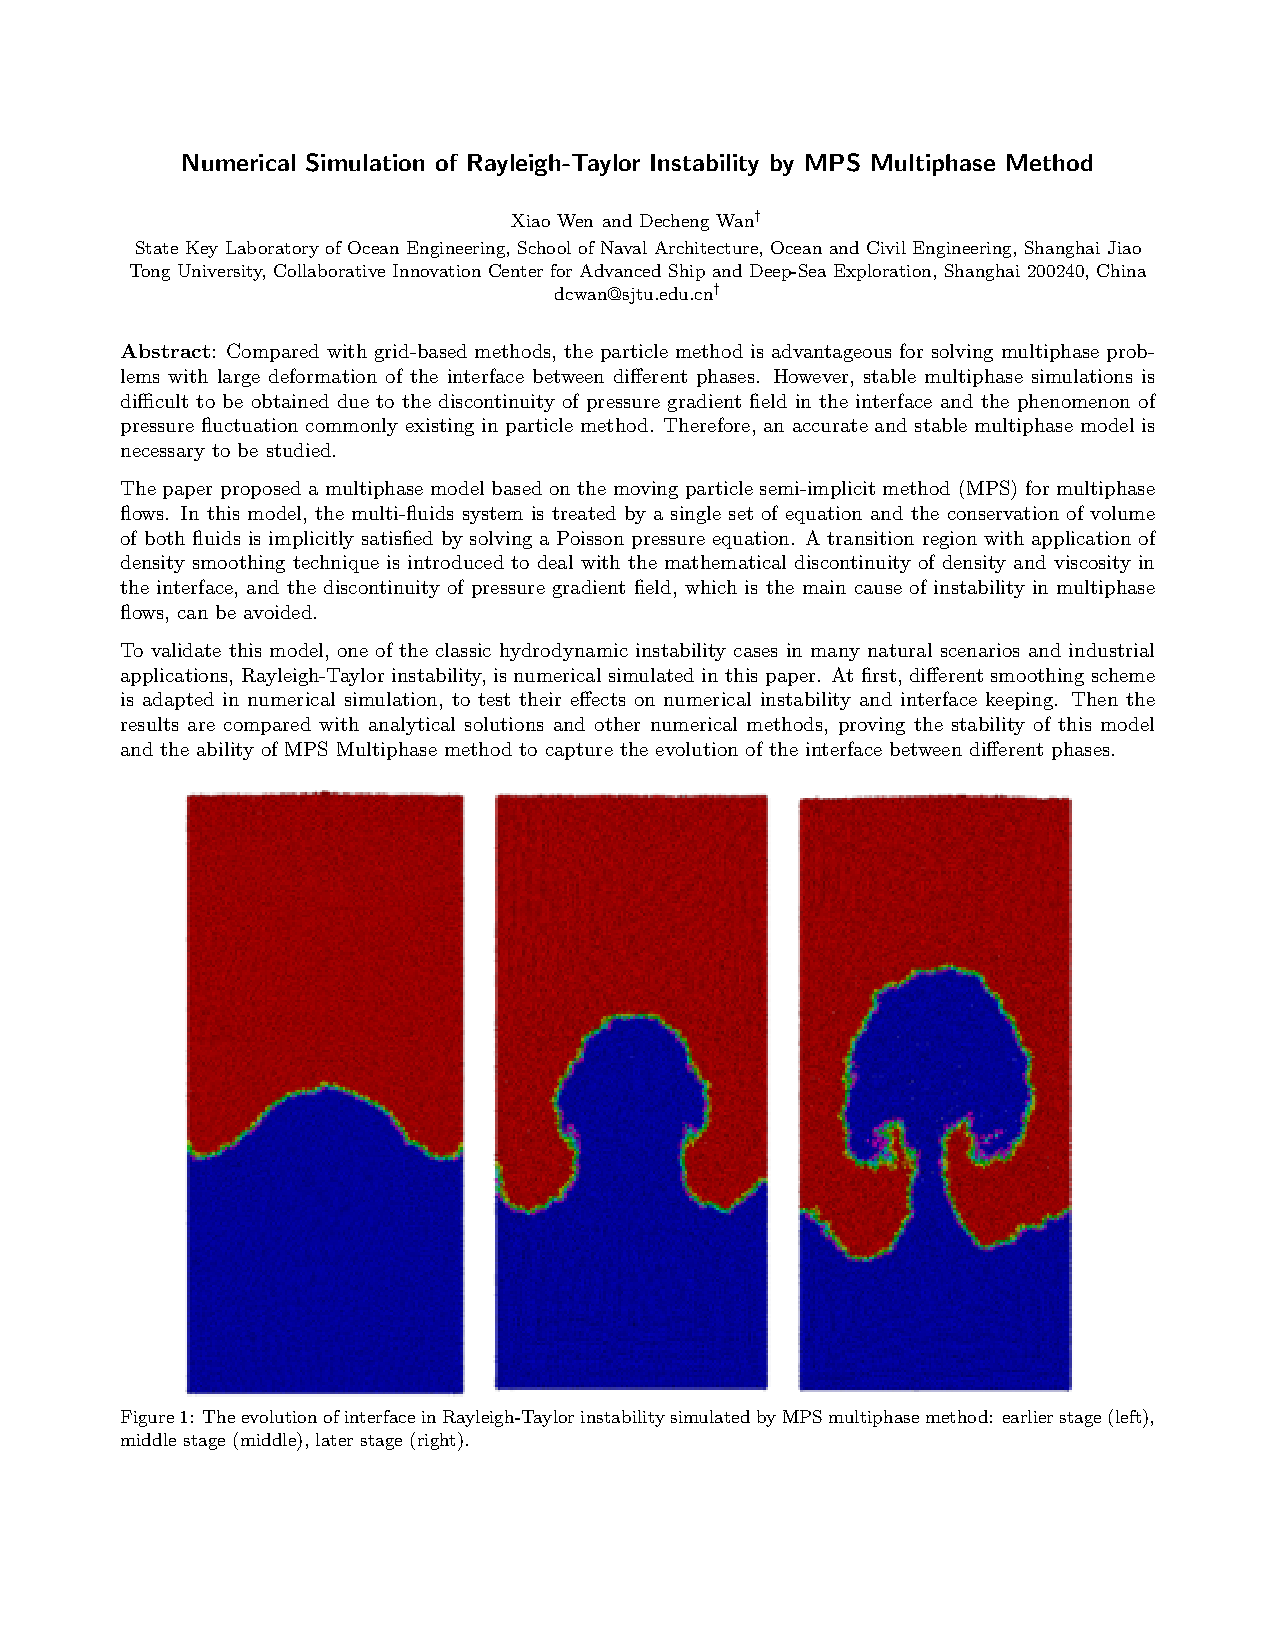
\includepdf[pages=-,pagecommand={\pagestyle{fancy}\label{12.4}},addtotoc={  
     1,subsection,1,Numerical simulation of Rayleigh-Taylor instability by MPS multiphase method,p1}]{abstract/pdfs/18.pdf}



%\section{Session 13: Alternative Formulations and Particle-Based Simulation Techniques}
%13.1: 35
%13.2: 56
%13.3: 13
%13.4: 23

\rhead{Session 13}
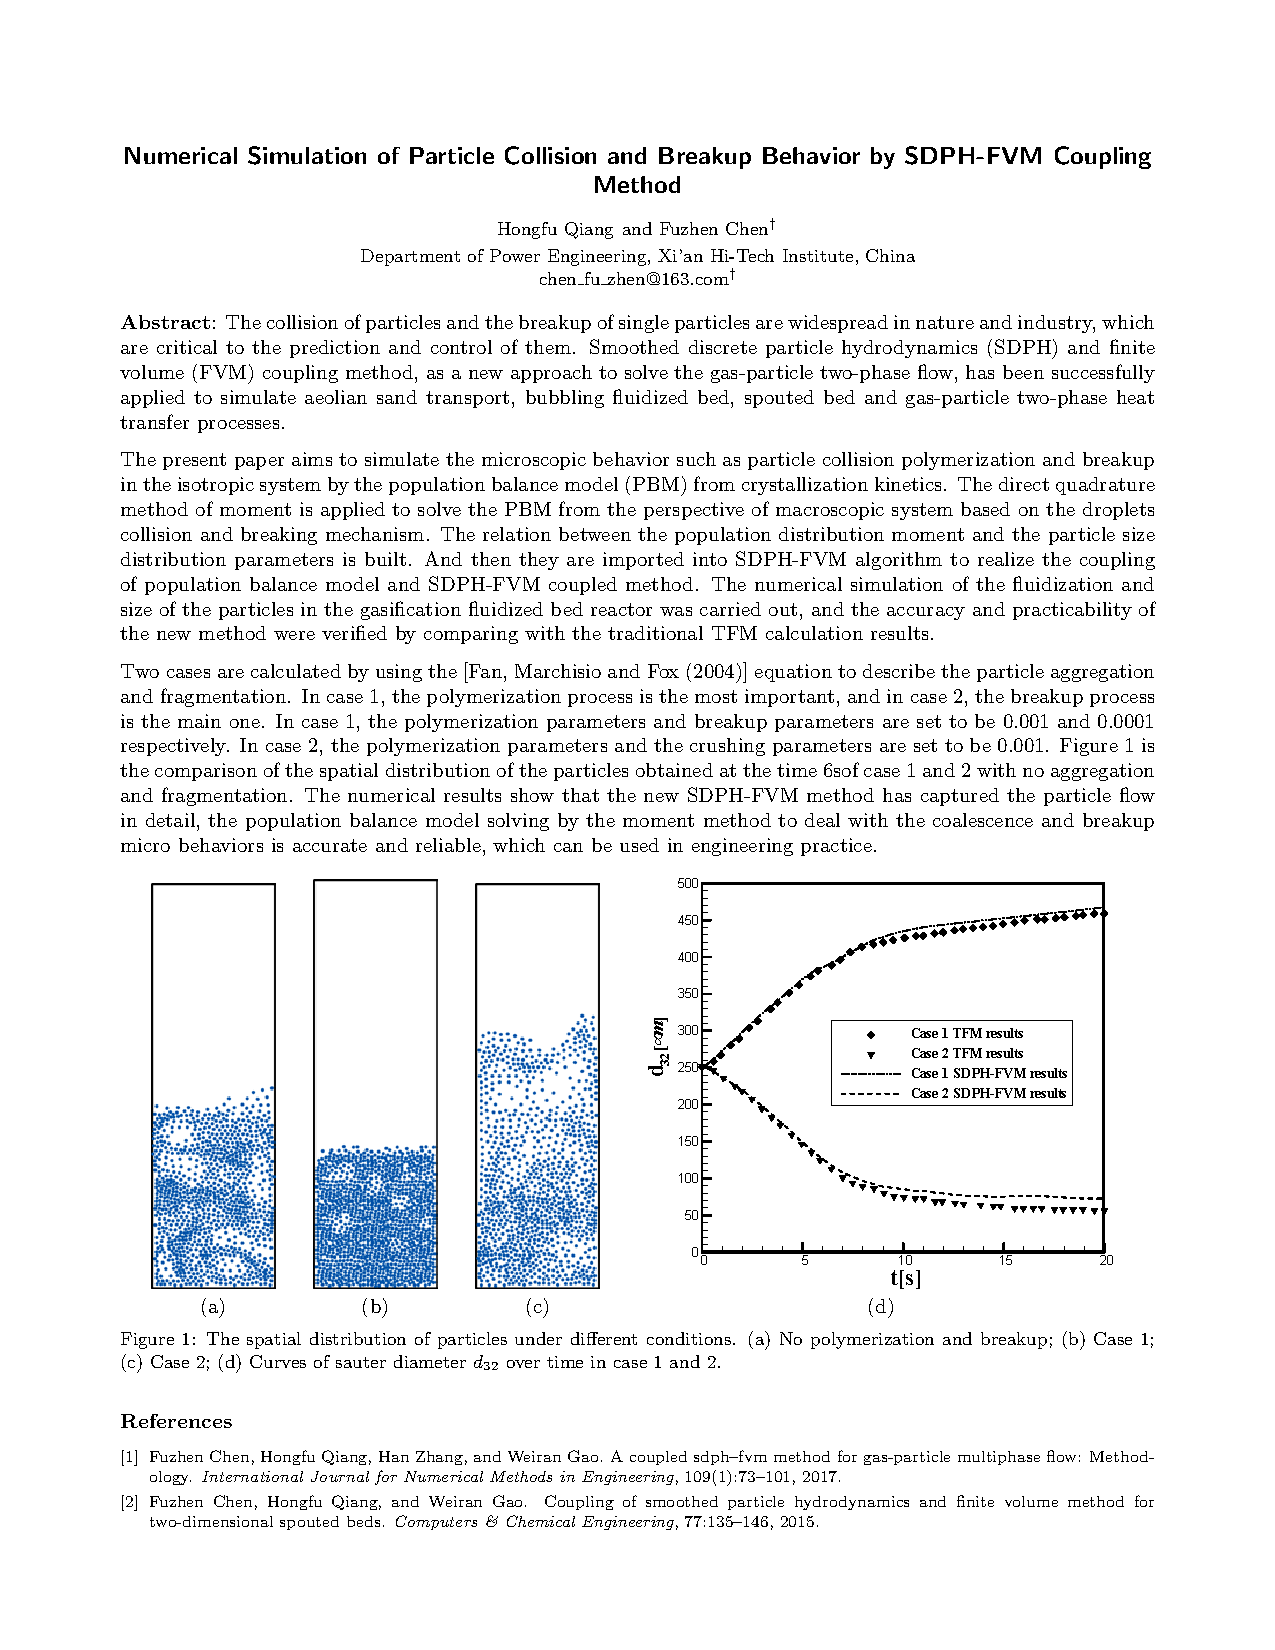
\includepdf[pages=-,pagecommand={\pagestyle{fancy}\label{13.1}},addtotoc={
     1,section,1,{~~~~~~~~Alternative Formulations and Particle-Based Simulation Techniques},p1,   
     1,subsection,1,Numerical simulation of particle collision and breakup behavior by SDPH-FVM coupling method,p1}]{abstract/pdfs/35.pdf}
\includepdf[pages=-,pagecommand={\pagestyle{fancy}\label{13.2}},addtotoc={  
     1,subsection,1,A physics evoked meshfree method,p1}]{abstract/pdfs/56.pdf}
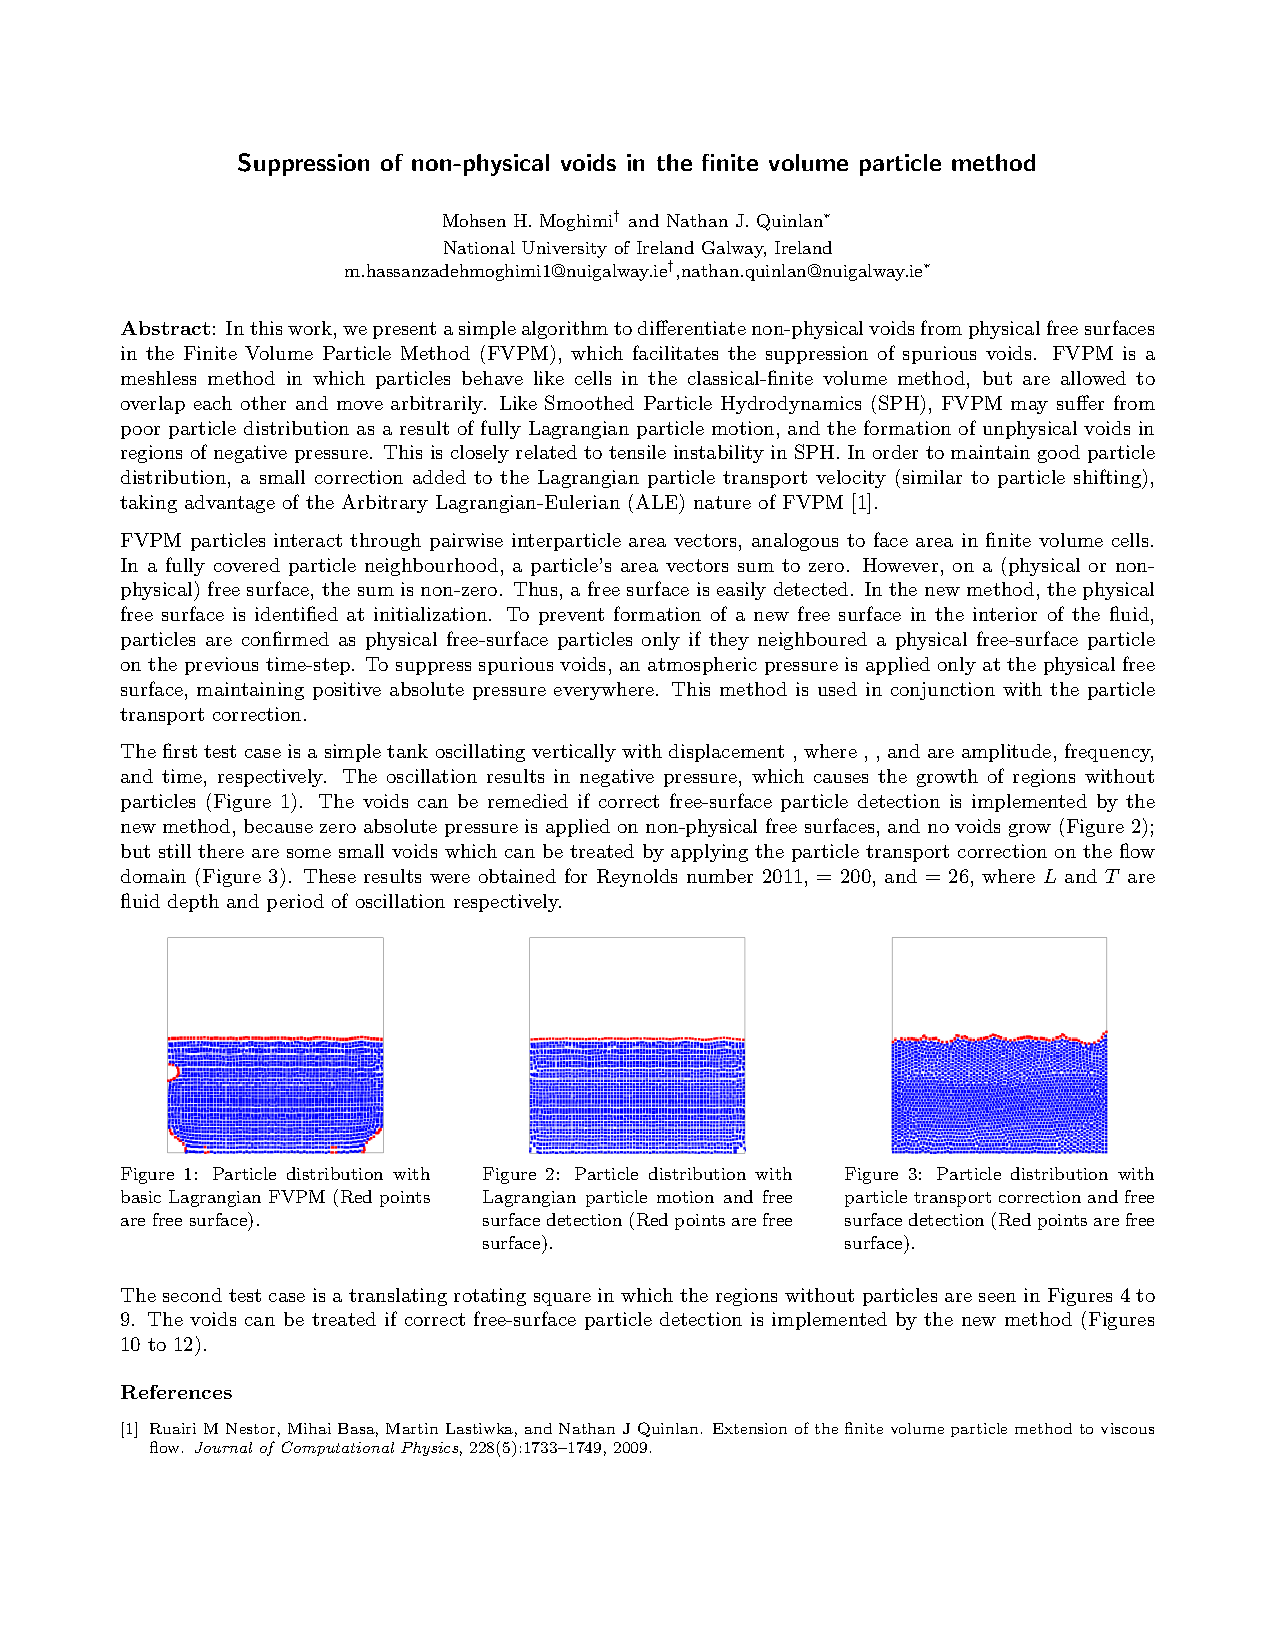
\includepdf[pages=-,pagecommand={\pagestyle{fancy}\label{13.3}},addtotoc={  
     1,subsection,1,Suppression of non-physical voids in the finite volume particle method,p1}]{abstract/pdfs/13.pdf}
\includepdf[pages=-,pagecommand={\pagestyle{fancy}\label{13.4}},addtotoc={  
     1,subsection,1,The Hermit-type RRKPM for piezoelectric materials,p1}]{abstract/pdfs/23.pdf}

%\section{Session 14: Other applications of SPH}
%14.1: 47
%14.2: 34
%14.3: 54
%14.4: 51

\rhead{Session 14}
\includepdf[pages=-,pagecommand={\pagestyle{fancy}\label{14.1}},addtotoc={
     1,section,1,{~~~~~~~~Other applications of SPH},p1,   
     1,subsection,1,A development of a SPH model for simulation of abrasive-water-jet impacting on a metallic surface,p1}]{abstract/pdfs/47.pdf}
\includepdf[pages=-,pagecommand={\pagestyle{fancy}\label{14.2}},addtotoc={  
     1,subsection,1,SPH simulation of Couette flow with sinusoidally moving solid boundary,p1}]{abstract/pdfs/34.pdf}
\includepdf[pages=-,pagecommand={\pagestyle{fancy}\label{14.3}},addtotoc={  
     1,subsection,1,Application of particle-based computational acoustics to sound propagation and scattering,p1}]{abstract/pdfs/54.pdf}
\includepdf[pages=-,pagecommand={\pagestyle{fancy}\label{14.4}},addtotoc={  
     1,subsection,1,Image processing with the SPH method,p1}]{abstract/pdfs/51.pdf}

%\section{Session 15: Hydraulic Applications II}
%15.1: 8 
%15.2: 20
%15.3: 28
%15.4: 53

\rhead{Session 15}
\includepdf[pages=-,pagecommand={\pagestyle{fancy}\label{15.1}},addtotoc={
     1,section,1,{~~~~~~~~Hydraulic Applications II},p1,   
     1,subsection,1,Analysis of the hydrological safety of dams using numerical tools: Iber and DualSPHysics,p1}]{abstract/pdfs/8.pdf}
\includepdf[pages=-,pagecommand={\pagestyle{fancy}\label{15.2}},addtotoc={  
     1,subsection,1,Construction of two-dimensional SPH numerical wave tank,p1}]{abstract/pdfs/28.pdf}
\includepdf[pages=-,pagecommand={\pagestyle{fancy}\label{15.3}},addtotoc={  
     1,subsection,1,An SPH numerical wave-current tank,p1}]{abstract/pdfs/53.pdf}
     
     
     
\rhead{Without presentation}

\includepdf[pages=-,pagecommand={\pagestyle{fancy}}]{abstract/pdfs/32.pdf}

